\chapter{Wind Turbine Control}  \label{sec:Application to Wind Turbine Control4} 
Modern megawatt wind turbines are both speed-controlled and pitch-controlled \cite{pao2011control,mulders2018delft, elkodama2023control}. Controllers and their parameters are often fine-tuned to
fit not only a specific wind turbine type but also individual turbines, taking into account factors
such as manufacturing and installation variations, including rotor blade weight imbalances and
aging processes \cite{en14238083}. These conventional feedback control designs, typically relying
solely on generator speed as input and controlling the blade pitch angles collectively, are
well-engineered and technologically mature. However, further reduction of the cost of energy
production can be achieved by introducing additional control inputs or sensors. Moreover, using a
predictive scheme like qLMPC allows leveraging wind measurements or estimates and incorporating
this information over a prediction horizon. It also accounts for how the system states, e.g., the
rotor and generator speed, are expected to react to the wind trajectory and future control inputs
within that horizon. This chapter investigates control strategies that leverage such improvements:
a qLMPC design, which incorporates wind information, and PI Individual Pitch Control
(IPC), the latter both as a standalone method and in combination with Trailing Edge Flap Control
(TEFC), aimed at reducing mechanical loads. These control approaches are evaluated in terms of
power reference tracking, actuator activity, and mechanical loads.
%
In Section~\ref{sec:quasiLPVMPCDesign}, the design of a velocity-based qLMPC controller based on
the first-principles model of Chapter~\ref{sec:WindTurbineqLPVModels} is presented. Whereas qLMPC
has so far been applied to wind turbines as a SISO scheme \cite{mulders2020preventing, pamososuryo2022individual,
    fonseca2024windTurbineSideSide}, the design presented here actuates generator torque and
collective pitch simultaneously as a MIMO scheme, covering the entire operating range. It is
reformulated as a QP and solved via a linear complementarity formulation with Lemke's algorithm
\cite{cisneros2020velocity}, yielding mean solver times below 2\,ms at a controller sampling time
of 8\,ms and thus real-time capability.
%
Section~\ref{section:Individal Pitch PI Control} introduces IPC, explaining the multiblade
coordinate transformation and comparing IPC simulation results to those from baseline Collective
Pitch Control (CPC). The simulation environment is also used to tune the IPC gains by a Nelder-Mead simplex optimization of the blade root Damage Equivalent Load (DEL), followed by
a constrained optimization that limits the tower base DEL.
%
Section~\ref{sec:CombinedIPC-TrailingEdgeFlapControl} describes the combination of IPC and TEFC, in the following called Active Aerodynamic Load Control (AALC), including the necessary model extensions and the achieved load reductions on the blades and tower. Whereas earlier studies combining the two actuation principles report results for single mean wind
speeds \cite{wilson2009combined, henriksen2013model, he2018combined}, the controller presented
here is demonstrated across Regions II and III, using one training dataset and two independent
verification datasets.
%
Section~\ref{subsec:ComparisonWindTurbineControlDesigns} compares qLMPC, IPC, and AALC, discussing the potential of the different schemes and showing the trade-offs between DEL reduction and actuator activity relative to the PI CPC
baseline. 
The results for the qLMPC applied to the qLPV model presented in Chapter~\ref{sec:WindTurbineqLPVModels} have been published in \cite{dittmer2021velocity}. They are extended here with results of the qLMPC applied to FAST and with modifications to the algorithm that improve its performance when applied to FAST. The AALC strategy has been published in \cite{dittmer2024combined}. It is extended here by a detailed discussion of the optimization of an IPC algorithm without Trailing Edge Flaps (TEFs), fine-tuned in the simulation environment of the AALC. The AALC parameters are re-optimized leveraging the IPC parameters optimized before.

%The results for the qLMPC controller have been published in \cite{dittmer2021velocity}, and the AALC control strategy in \cite{dittmer2024combined}.

\section{qLMPC Design and Application}\label{sec:quasiLPVMPCDesign} 
Wind turbine controller design in the above-rated region focuses on smooth power control and in the below-rated region on power optimization, as described in \cite{Bianchi2007}. The proposed MIMO qLMPC uses two control inputs, the collective pitch command $\beta_{0,\text{ref}}$ and the generator torque reference $T_{g,\text{ref}}$. The baseline controller consists of two SISO controllers, one for generator torque and one for blade pitch control, see Section~\ref{sec:WindTurbineControl}. These can be replaced by a MIMO qLMPC controller, see Figure~\ref{fig:BlockMPC}. 
\begin{figure}[ht]
    \centering
    \includegraphics[width=0.7\textwidth,trim={0 0cm 0cm 0.1cm},clip]{figures/Figures_ADi/turbineCtrlBetaMPC1.pdf}
    \caption[Block diagram of qLMPC replacing the baseline PI controller]{Block diagram of qLMPC replacing the baseline PI controller: the baseline gain-scheduled pitch controller $PI_{GS}(\omega_g)$ and torque controller $k\omega_g^2$ (solid boxes) are replaced by the qLMPC (dashed box). Based on the measured generator speed $\omega_g$ and the estimated wind speed~$\hat{V}_\infty$, it sets the collective pitch reference $\beta_{0,\text{ref}}$ and the generator torque reference $T_{g,\text{ref}}$.}   
    \label{fig:BlockMPC}
\end{figure}
% \caption[Block diagram of the closed-loop wind turbine control structure with qLMPC replacing the baseline PI controller]{Block diagram of the closed-loop wind turbine control structure with qLMPC (dashed box) replacing the baseline PI controller (solid line)}
%
Optimal reference signals $r_\beta$ and $r_{T_g}$ for the two actuator states are calculated from the wind speed $V_\infty$. The cost function penalizes the deviation of the actuator signals $\beta_{0,\text{ref}}$ and  $T_{g,\text{ref}}$ from $r_\beta$ and $r_{T_g}$, the changes of the rotor and generator speed, which in the velocity-based form drive the system to a steady state, and the changes in the control inputs. On the qLPV model, this results in smoother power output and reduced tower movement compared to the baseline. DEL reduction is not an explicit objective of the qLMPC design. However, the six evaluation criteria used to compare all control strategies introduced in Section~\ref{subsection: IPCOptCriteria}, i.e., blade, tower base and tower top DEL, power mean and variance, and actuator activity, are also calculated for this controller to enable a direct comparison with the IPC and AALC designs.

In this work, the velocity-based approach from \cite{cisneros2020velocity}, presented in Section~\ref{sec:qLPVmodels} of this thesis, is applied to a model based on the wind turbine model used for qLPV-based MIMO controller design in \cite{Bianchi2007}. The model in \cite{Bianchi2007} contains three turbine states, the slip angle $\theta_s$ and the rotor and generator speed $\omega_r$ and $\omega_{gr}$, as well as the pitch actuator state $\beta_0$. These four states are a subset of the state vector of the extended model Mdl2$^\prime$ in Equation~\eqref{eq:11} and are sufficient to control the power output. Smoother rotor speed and pitch activity also reduce thrust variations and thus, indirectly, tower and blade movement. Hence, for the sake of simplicity, the decision was made to base the qLMPC scheme on a model close to the one in \cite{Bianchi2007} instead of the extended model Mdl2$^\prime$, as the lower model order reduces the size of the optimization problem and thus the computation time. As control inputs, \cite{Bianchi2007} uses the blade pitch command $\beta_{0,\text{ref}}$ and the zero torque speed $\omega_Z$, which is linearly dependent on the generator torque $T_g$. Three modifications are made to this model:
\begin{enumerate}
    \item The reference generator torque $T_{g,\text{ref}}$ is used as the second control input instead of $\omega_Z$. The reference torque is selected because FAST expects a torque command as input. The optimal trajectory of the reference generator torque $T_{g,\text{ref}}$ over a prediction horizon is calculated based on an optimal reference signal $r_{T_g}$, which is itself calculated from the wind speed.
    \item The generator torque $T_g$, which lags the commanded control signal $T_{g,\text{ref}}$, is used as an additional state to eliminate direct feedthrough, i.e., to avoid a non-zero feedthrough matrix. This fifth state enables the use of the optimization framework for reference tracking and disturbance rejection proposed in \cite{cisneros2020velocity}. Incorporating a filtered control input as an additional state is a common practice, and is, for example, also employed in the MPC algorithm implemented in the Wind Farm Simulator (WFSim) \cite{boersma2018control}. %~\(\bm{D} \)
    \item A desired pitch signal $r_{\beta}$ is used as a reference for the prediction horizon in the MPC optimization to calculate the optimal pitch command $\beta_{0,\text{ref}}$. In \cite{Bianchi2007}, a reference value for the generator speed is tracked. This choice was made to directly optimize the two actuators to avoid handling the large difference in dynamic bandwidth of the actuators and the plant dynamics in the optimization calculation.
\end{enumerate}
%
The resulting state, input and output vectors are given below. As before, different indices are used for the generator speed on the high-speed shaft, denoted $\omega_g$, and the generator speed referred to the low-speed shaft, $\omega_{gr}$. In the state vector, $\omega_{gr}$ is used, as it is in the same reference frame as the rotor speed $\omega_r$:
\begin{equation}\label{eq:xMPCyMPC}
    \begin{aligned}
        \bm{x}_{\text{MPC}} &= [\theta_{s} \quad \omega_r \quad \omega_{gr} \quad T_g \quad \beta_0]^T \in \mathbb{R}^{5 \times 1},\\
        \bm{w}_{\text{Mdl}^\prime} &= [V_{\infty} \quad T_{g,\text{ref}} \quad \beta_{0,\text{ref}}]^T \in \mathbb{R}^{3 \times 1}, \quad
        \bm{y}_{\text{MPC}} = [T_g \quad \beta_0]^T \in \mathbb{R}^{2 \times 1}.
    \end{aligned}
\end{equation}
%
Note that $\bm{y}_{\text{MPC}}$ contains the outputs of the prediction model, i.e., the controlled variables tracked in the cost function, whereas the outputs of the controller are the commanded signals $T_{g,\text{ref}}$ and $\beta_{0,\text{ref}}$ in $\bm{w}_{\text{Mdl}^\prime}$. The nonlinear dynamics of the three turbine states and the two actuator states are:
\begin{align}
    \dot{\theta}_s(t) &= \omega_r(t)-\omega_{gr}(t) \label{eq:NLDyn1},\\
    \dot{\omega}_r(t) &= -\frac{K_{sr}}{J_r}\theta_s(t)-\frac{B_{sr}}{J_r}\omega_r(t)+\frac{B_{sr}}{J_r}\omega_{gr}(t)+\frac{T_r(\omega_r, \beta_0, V_\infty)}{J_r},\\
    \dot{\omega}_{gr}(t) &= \frac{K_{sr}}{J_{gr}}\theta_s(t)+\frac{B_{sr}}{J_{gr}}\omega_r(t)-\frac{B_{sr}}{J_{gr}}\omega_{gr}(t)-\frac{N_g T_g(t)}{J_{gr}} \label{eq:NLDyn3},\\
    \dot{T}_{g}(t) &= -\frac{1}{\kappa}T_{g}(t)+\frac{1}{\kappa}T_{g,\text{ref}}(t),\\
    \dot{\beta}_0(t) &= -\frac{1}{\tau}\beta_0(t)+\frac{1}{\tau}\beta_{0,\text{ref}}(t).\label{eq:NLDyn5}
\end{align}
%
To avoid having to derive a grid of equilibrium points for the different combinations of the state vector, a velocity-based linearization is used.

\subsection{Velocity-Based qLPV Model for Reference Tracking}
The velocity-based linearization method from \cite{cisneros2020velocity}, introduced in Section~\ref{sec:qLPVmodels}, is implemented for the model serving as the basis of the qLMPC design. The nonlinear system dynamics
\[
\dot{\bm{x}}_{\text{MPC}}(t) = \bm{f}_{\text{MPC}}(\bm{x}_{\text{MPC}}, \bm{w}_{\text{Mdl}^\prime}), \quad \bm{y}_{\text{MPC}}(t) = \bm{h}_{\text{MPC}}(\bm{x}_{\text{MPC}})
\]
are described by the relationship between the derivatives of the states, inputs, and outputs:
\begin{align*}
    \ddot{\bm{x}}_{\text{MPC}}(t) &= \nabla_{\bm{x}_{\text{MPC}}} \bm{f}_{\text{MPC}}(\bm{x}_{\text{MPC}}, \bm{w}_{\text{Mdl}^\prime}) \dot{\bm{x}}_{\text{MPC}}(t) + \nabla_{\bm{w}_{\text{Mdl}^\prime}} \bm{f}_{\text{MPC}}(\bm{x}_{\text{MPC}}, \bm{w}_{\text{Mdl}^\prime}) \dot{\bm{w}}_{\text{Mdl}^\prime}(t),\\
    \dot{\bm{y}}_{\text{MPC}}(t) &= \nabla_{\bm{x}_{\text{MPC}}} \bm{h}_{\text{MPC}}(\bm{x}_{\text{MPC}}) \dot{\bm{x}}_{\text{MPC}}(t).
\end{align*}
By considering the derivatives instead of the original states, the need for storing steady-state vectors for input, output, and states at each operating point is eliminated.
As in the actuator-augmented model in Equation~\eqref{eq:11}, the input vector $\bm{w}_{\text{Mdl}^\prime} = [V_{\infty} \;\; T_{g,\text{ref}} \;\; \beta_{0,\text{ref}}]^T$ contains the commanded signals, and the actuator outputs $T_g$ and $\beta_0$ are states.
%
The continuous-time system, input, and output matrices are
\begin{align*}
    \bm{A}_c(\bm{\rho}_\Rho) &= \nabla_{\bm{x}_{\text{MPC}}} \bm{f}_{\text{MPC}}(\bm{x}_{\text{MPC}}, \bm{w}_{\text{Mdl}^\prime}),\quad
    \bm{B}_c(\bm{\rho}_\Rho) = \nabla_{\bm{w}_{\text{Mdl}^\prime}} \bm{f}_{\text{MPC}}(\bm{x}_{\text{MPC}}, \bm{w}_{\text{Mdl}^\prime}),\\
    \bm{C}_c &= \nabla_{\bm{x}_{\text{MPC}}} \bm{h}_{\text{MPC}}(\bm{x}_{\text{MPC}}),
\end{align*}
with the state vector $\bm{x}_{\text{MPC}}$ and output vector $\bm{y}_{\text{MPC}}$ as defined in Equation~\eqref{eq:xMPCyMPC}. Since $\bm{y}_{\text{MPC}}$ consists of two states, $\bm{C}_c$ is constant. The scheduling parameter vector consists of the wind speed $V_{\infty}$, the pitch angle $\beta_0$, and the rotor speed $\omega_r$,
\begin{equation} \label{eq:rhoWT4}
    \bm{\rho}_\Rho = [V_{\infty} \quad \beta_0 \quad \omega_{r}]^T \in \mathbb{R}^{3 \times 1}.
\end{equation}
At the current time step, the measured or estimated values are used. Over the prediction horizon, $\omega_r$ and $\beta_0$ are taken from the predicted trajectories of the previous optimization step, while $V_{\infty}$ is held constant. Although the control scheme is velocity-based, i.e., based on state derivatives or, in discrete time, state differences, the scheduling parameters are taken in their original non-derivative form. This is because partial derivatives such as \( \partial T_r / \partial \omega_r \), \( \partial T_r / \partial \beta_0 \), and \( \partial T_r / \partial V_{\infty} \) are functions of the current physical states, not of their time derivatives.

The matrices depend on the physical parameters described in Section~\ref{sec:MechanicalAerodynamicSubsystemModel} and can be set up from Equations~\eqref{eq:NLDyn1} to~\eqref{eq:NLDyn5}:
\begin{equation}
    \begin{aligned}
        \bm{A}_c(\bm{\rho}_{\Rho}) &=
        \begin{bmatrix}
            0  & 1 & -1 & 0 & 0 \\ 
            -\frac{K_{sr}}{J_r}  & -\frac{B_{sr}}{J_r} + \frac{1}{J_r}\frac{\partial T_r}{\partial{\omega_r}} & \frac{B_{sr}}{J_r} & 0 & \frac{1}{J_r}\frac{\partial T_r}{\partial \beta_0} \\
            \frac{K_{sr}}{J_{gr}} & \frac{B_{sr}}{J_{gr}} & -\frac{B_{sr}}{J_{gr}} & -\frac{N_g}{J_{gr}} & 0 \\ 
            0 & 0 & 0 & -\frac{1}{\kappa} & 0 \\ 
            0 & 0 & 0 & 0 & -\frac{1}{\tau} 
        \end{bmatrix} \in \mathbb{R}^{5 \times 5},\\
        \bm{B}_c(\bm{\rho}_{\Rho}) &=
        \left[
        \begin{array}{c|cc}
            0 & 0 & 0 \\
            \frac{1}{J_r}\frac{\partial T_r}{\partial V_{\infty}} & 0 & 0 \\
            0 & 0 & 0 \\
            0 & \frac{1}{\kappa} & 0 \\
            0 & 0 & \frac{1}{\tau}
        \end{array}
        \right]
        =
        \begin{bmatrix}
            \bm{B}_{c,V} & \bm{B}_{c,u}
        \end{bmatrix}
        \in \mathbb{R}^{5 \times 3},\\
        \bm{C}_c &=
        \begin{bmatrix}
            0 & 0 & 0 & 1 & 0 \\
            0 & 0 & 0 & 0 & 1
        \end{bmatrix} \in \mathbb{R}^{2 \times 5}.
    \end{aligned}
\end{equation}
%
The wind affects the system through the first column of the input matrix, denoted here as $\bm{B}_{c,V}$. The wind speed $V_{\infty}$ cannot be controlled and only its current value is assumed to be known and constant over the prediction horizon. Nevertheless, the column $\bm{B}_{c,V}$ must be retained, as the change in wind speed $\Delta V_{\infty}$ is treated as a disturbance input between time steps. To reflect this structure, the input matrix $\bm{B}_c$ is partitioned into the wind disturbance input $\bm{B}_{c,V}$ in the first column and the control input influence $\bm{B}_{c,u}$ in the second and third columns. For implementation in the predictive controller, the wind speed change $\Delta V_{\infty}$ is moved into the system matrix as an additional state, since it represents a known but uncontrollable input.

This continuous-time qLPV model needs to be discretized for its application in a real-time qLMPC design. The model in discretized form is:
\begin{align}\label{eq4:DiscreteForm}
    \Delta \bm{x}_{\text{MPC}}(k+1) = \bm{A}_{d}(\bm{\rho}_\Rho)\Delta \bm{x}_{\text{MPC}}(k) + \bm{B}_{d}(\bm{\rho}_\Rho) \Delta \bm{w}_{\text{Mdl}^\prime}(k)
\end{align}
with the discretized system and input matrices $\bm{A}_d \in \mathbb{R}^{5 \times 5}$ and $\bm{B}_d \in \mathbb{R}^{5 \times 3}$ dependent on the scheduling parameter vector $\bm{\rho}_{\Rho}$ at the $k$-th sample.
%
%
As in \cite{cisneros2019wide}, the discrete-time matrices $\bm{A}_d$ and $\bm{B}_d$ in Equation~\eqref{eq:zoh1} are approximated by truncating their series expansion after the fourth-order term. The discrete-time system and input matrices used here are therefore:
\begin{align*}
    \bm{A}_{d}(\bm{\rho}_\Rho) &= \frac{T_s^4}{24}\bm{A}_c^4(\bm{\rho}_\Rho) + \frac{T_s^3}{6}\bm{A}_c^3(\bm{\rho}_\Rho) + \frac{T_s^2}{2}\bm{A}_c^2(\bm{\rho}_\Rho) + T_s \bm{A}_c(\bm{\rho}_\Rho) + \bm{I},\\
    \bm{B}_{d}(\bm{\rho}_\Rho) &= \left( \frac{T_s^4}{24}\bm{A}_c^3(\bm{\rho}_\Rho) + \frac{T_s^3}{6}\bm{A}_c^2(\bm{\rho}_\Rho) + \frac{T_s^2}{2}\bm{A}_c(\bm{\rho}_\Rho) + T_s \bm{I} \right) \bm{B}_c(\bm{\rho}_\Rho).
\end{align*}
%
The discrete-time outputs can be calculated as the sum of the former sampled outputs and their current change:
\begin{align*}
    T_{g}(k+1) = T_{g}(k) + \Delta T_{g}(k+1), \quad \beta_{0}(k+1) = \beta_{0}(k) + \Delta \beta_{0}(k+1).
\end{align*}
%
Including the output signal values, the discrete state at step $k+1$ is calculated as presented in Equation~\eqref{eq:discreteVelocityqLPV}:
\begin{equation} \label{eq:discreteVelocityqLPV4}
    \begin{bmatrix}
        \bm{y}_{\text{MPC}}(k+1) \\
        \Delta \bm{x}_{\text{MPC}}(k+1)
    \end{bmatrix} = \begin{bmatrix}
        \bm{I}_{2\times2} & \bm{A}_{d,y}(\bm{\rho}_\Rho) \\
        \bm{0}_{5\times2} & \bm{A}_{d}(\bm{\rho}_\Rho)
    \end{bmatrix} \begin{bmatrix}
        \bm{y}_{\text{MPC}}(k) \\
        \Delta \bm{x}_{\text{MPC}}(k)
    \end{bmatrix} + \begin{bmatrix}
        \bm{B}_{d,y}(\bm{\rho}_\Rho) \\
        \bm{B}_{d}(\bm{\rho}_\Rho)
    \end{bmatrix} \Delta \bm{w}_{\text{Mdl}^\prime}(k)
\end{equation}
with $\bm{A}_{d,y} = \bm{C}_c\bm{A}_d \in \mathbb{R}^{2 \times 5}$ and $\bm{B}_{d,y} = \bm{C}_c\bm{B}_d \in \mathbb{R}^{2 \times 3}$ denoting the rows of the matrices corresponding to the outputs. Here, $\bm{C}_c$ is the output matrix of the continuous-time model, which selects the two actuator states $T_g$ and $\beta_0$ from $\bm{x}_{\text{MPC}}$.
The resulting intermediate state vector is
\begin{align*}
    \tilde{\bm{x}}_{\text{MPC}} = \begin{bmatrix} \bm{y}_{\text{MPC}}^T & \Delta\bm{x}_{\text{MPC}}^T \end{bmatrix}^T = \begin{bmatrix} T_{g} & \beta_{0} & \Delta \theta_{s} & \Delta \omega_{r} & \Delta \omega_{gr} & \Delta T_{g} & \Delta \beta_{0} \end{bmatrix}^T \in \mathbb{R}^{7 \times 1}.
\end{align*}
%
Since the optimization can only determine the control inputs and the wind speed acts as an uncontrollable disturbance, the input vector $\bm{w}_{\text{Mdl}^\prime}$ and the input matrix are split into a disturbance part and a control part.
The control input vector $\bm{u}_{\text{Mdl}^\prime} = [T_{g,\text{ref}} \;\; \beta_{0,\text{ref}}]^T$ consists of the two control inputs contained in $\bm{w}_{\text{Mdl}^\prime} = [V_{\infty} \;\; T_{g,\text{ref}} \;\; \beta_{0,\text{ref}}]^T$, with its discrete-time velocity-based form
\begin{align} \label{eq:DeltaUinput}
    \Delta \bm{u}_{\text{Mdl}^\prime} = \begin{bmatrix} \Delta T_{g,\text{ref}} & \Delta \beta_{0,\text{ref}} \end{bmatrix}^T.
\end{align}
%
For MPC, the augmented discrete-time state-space model can be written as:
\begin{equation*}
    \begin{aligned}
        \begin{bmatrix}
            \bm{y}_{\text{MPC}}(k+1) \\
            \Delta \bm{x}_{\text{MPC}}(k+1)
        \end{bmatrix} &= \begin{bmatrix}
            \bm{I}_{2\times2} & \bm{A}_{d,y}(\bm{\rho}_\Rho) \\
            \bm{0}_{5\times2} & \bm{A}_d(\bm{\rho}_\Rho)
        \end{bmatrix}
        \begin{bmatrix}
            \bm{y}_{\text{MPC}}(k) \\
            \Delta \bm{x}_{\text{MPC}}(k)
        \end{bmatrix}
        +
        \begin{bmatrix}
            \bm{B}_{d,y,V}(\bm{\rho}_\Rho) \\
            \bm{B}_{d,V}(\bm{\rho}_\Rho)
        \end{bmatrix} \Delta V_{\infty}(k) \\
        &\quad +
        \begin{bmatrix}
            \bm{B}_{d,y,u}(\bm{\rho}_\Rho) \\
            \bm{B}_{d,u}(\bm{\rho}_\Rho)
        \end{bmatrix} \Delta \bm{u}_{\text{Mdl}^\prime}(k)
    \end{aligned}
\end{equation*}
where $\bm{B}_{d,V} \in \mathbb{R}^{5 \times 1}$ and $\bm{B}_{d,u} \in \mathbb{R}^{5 \times 2}$ are the columns of the input matrix related to the changes in the disturbance input, i.e., wind speed $\Delta V_{\infty}$, and the two control inputs, respectively, acting on the changes in states. The matrices $\bm{B}_{d,y,V} = \bm{C}_c\bm{B}_{d,V} \in \mathbb{R}^{2 \times 1}$ and $\bm{B}_{d,y,u} = \bm{C}_c\bm{B}_{d,u} \in \mathbb{R}^{2 \times 2}$ directly influence the two outputs $T_g$ and $\beta_0$ in the vector $\bm{y}_{\text{MPC}}$. 

The wind is considered to only change at the first sample of the prediction horizon. This reflects that the wind measurement or estimate at each controller sample might be different from the last controller sample, but that the wind is then, in the absence of better information, assumed to be constant over the prediction horizon. The wind change $\Delta V_{\infty}$ is implemented as an eighth state:
\begin{equation} \label{eq:AugmentedStateSpace}
    \begin{aligned}
        \begin{bmatrix}
            \bm{y}_{\text{MPC}}(k+1) \\
            \Delta \bm{x}_{\text{MPC}}(k+1) \\
            \Delta V_{\infty}(k+1)
        \end{bmatrix}
        &=
        \underbrace{\begin{bmatrix}
                \bm{I}_{2\times2} & \bm{A}_{d,y}(\bm{\rho}_\Rho) & \bm{B}_{d,y,V}(\bm{\rho}_\Rho) \\
                \bm{0}_{5\times2} & \bm{A}_d(\bm{\rho}_\Rho) & \bm{B}_{d,V}(\bm{\rho}_\Rho) \\
                \bm{0}_{1\times2} & \bm{0}_{1\times5} & 0
        \end{bmatrix}}_{\bm{A}_{\Delta V}}
        \underbrace{\begin{bmatrix}
                \bm{y}_{\text{MPC}}(k) \\
                \Delta \bm{x}_{\text{MPC}}(k) \\
                \Delta V_{\infty}(k)
        \end{bmatrix}}_{\bm{x}_{\text{MPC},\Delta V}(k)} \\
        &\quad +
        \underbrace{
            \begin{bmatrix}
                \bm{B}_{d,y,u}(\bm{\rho}_\Rho) \\
                \bm{B}_{d,u}(\bm{\rho}_\Rho) \\
                \bm{0}_{1\times2}
        \end{bmatrix}}_{\bm{B}_{\Delta V}} \Delta \bm{u}_{\text{Mdl}^\prime}(k)
    \end{aligned}
\end{equation}
with the system matrix $\bm{A}_{\Delta V} \in \mathbb{R}^{8 \times 8}$, the input matrix $\bm{B}_{\Delta V} \in \mathbb{R}^{8 \times 2}$ and the state vector
\begin{align}\label{eq:AugmentedStateVector}
    \bm{x}_{\text{MPC},\Delta V} = \begin{bmatrix} T_g & \beta_0 & \Delta \theta_s & \Delta \omega_r & \Delta \omega_{gr} & \Delta T_g & \Delta \beta_0 & \Delta V_{\infty} \end{bmatrix}^T \in \mathbb{R}^{8 \times 1}.
\end{align}
Regarding the wind speed, two simplifying assumptions are made. First, the current wind speed is known exactly, i.e., $\hat{V}_\infty = V_\infty$. In the simulation, the undisturbed longitudinal wind speed at hub height, provided by the FAST InflowWind module, is passed directly to the qLMPC algorithm. Second, this wind speed is assumed to remain constant over the prediction horizon of 0.32\,s, that is 40 steps of 0.008\,s, consistent with $\Delta V_{\infty}(k+1) = 0$ in Equation~\eqref{eq:AugmentedStateSpace}. Neither wind preview nor a stochastic wind model is used. The second assumption is reasonable, as the wind speed changes only slightly over such short time scales.

In practical wind turbine operation, the wind speed is typically measured using nacelle-mounted anemometers, which provide local measurements at hub height but are affected by the rotor wake \cite{smith2002applicability}. A more advanced alternative is the spinner anemometer, mounted at the front of the rotor hub, which measures less disturbed inflow \cite{demurtas2017spinaranemometer}. Alternatively, the rotor-effective wind speed can be estimated from the measured generator speed, generator torque, and pitch angle using the aerodynamic model of the rotor \cite{soltani2013estimation}. Since these estimators are continuously corrected by the measured rotor speed, their error does not accumulate over time, but they are sensitive to errors in the aerodynamic model. Light Detection and Ranging (lidar) systems, although more costly, can measure the wind speed at multiple upstream locations and thus provide a wind preview, which is particularly valuable for MPC \cite{schlipf2013nonlinear}. As the focus of this work is on the qLMPC algorithm rather than on the benefits of wind preview, and no lidar simulation was readily available, only the current wind speed is used. This is conservative with respect to wind preview, while the exact knowledge of the current wind speed is optimistic compared to a real wind speed estimator.

Additionally, the actuator commands are applied with a delay of one sample, which is introduced in the simulation to avoid an algebraic loop between controller and plant. To account for this, the control increments from the last step, $\Delta \bm{u}_{\text{Mdl}^\prime}(k-1)$, are included in the state vector, so that the increment computed at step $k$ acts on the plant at step $k+1$. 
%\needspace{12\baselineskip}
With this, the discrete state at step $k+1$ is calculated as:
\begin{equation} \label{eq:FinalStateSpace}
    \begin{aligned}
        \begin{bmatrix}
            \bm{y}_{\text{MPC}}(k+1) \\
            \Delta \bm{x}_{\text{MPC}}(k+1) \\
            \Delta V_{\infty}(k+1) \\
            \Delta \bm{u}_{\text{Mdl}^\prime}(k)
        \end{bmatrix}
        &=
        \underbrace{\begin{bmatrix}
                \bm{I}_{2\times2} & \bm{A}_{d,y}(\bm{\rho}_\Rho) & \bm{B}_{d,y,V}(\bm{\rho}_\Rho) & \bm{B}_{d,y,u}(\bm{\rho}_\Rho) \\
                \bm{0}_{5\times2} & \bm{A}_{d}(\bm{\rho}_\Rho) & \bm{B}_{d,V}(\bm{\rho}_\Rho) & \bm{B}_{d,u}(\bm{\rho}_\Rho) \\
                \bm{0}_{1\times2} & \bm{0}_{1\times5} & 0 & \bm{0}_{1\times2} \\
                \bm{0}_{2\times2} & \bm{0}_{2\times5} & \bm{0}_{2\times1} & \bm{0}_{2\times2}
        \end{bmatrix}}_{\bm{A}_{\text{MPC}^\prime}}
        \underbrace{\begin{bmatrix}
                \bm{y}_{\text{MPC}}(k) \\
                \Delta \bm{x}_{\text{MPC}}(k) \\
                \Delta V_{\infty}(k) \\
                \Delta \bm{u}_{\text{Mdl}^\prime}(k-1)
        \end{bmatrix}}_{\bm{x}_{\text{MPC}^\prime}(k)} \\
        &\quad +
        \underbrace{\begin{bmatrix}
                \bm{0}_{2\times2} \\
                \bm{0}_{5\times2} \\
                \bm{0}_{1\times2} \\
                \bm{I}_{2\times2}
        \end{bmatrix}}_{\bm{B}_{\text{MPC}^\prime}}
        \Delta \bm{u}_{\text{Mdl}^\prime}(k),
    \end{aligned}
\end{equation}
with the system matrix $\bm{A}_{\text{MPC}^\prime} \in \mathbb{R}^{10 \times 10}$, the input matrix $\bm{B}_{\text{MPC}^\prime} \in \mathbb{R}^{10 \times 2}$ and the state vector $\bm{x}_{\text{MPC}^\prime}$ given in Equation~\eqref{eq:stateMPC}.
The control increment $\Delta\bm{u}_{\text{Mdl}^\prime}$ acts on the plant one sample later, reflecting the one-sample delay of the actuator commands. As before, $\Delta V_{\infty}(k+1) = 0$, so that the wind speed is constant over the prediction horizon. The new state vector is hence
\begin{align} \label{eq:stateMPC}
    \bm{x}_{\text{MPC}^\prime}(k) = \begin{bmatrix} \bm{y}_{\text{MPC}}^T(k) & \Delta\bm{x}_{\text{MPC}}^T(k) & \Delta V_{\infty}(k) & \Delta\bm{u}_{\text{Mdl}^\prime}^T(k-1) \end{bmatrix}^T \in \mathbb{R}^{10 \times 1},
\end{align}
or, explicitly,
\begin{align*}
    \bm{x}_{\text{MPC}^\prime,k} = \begin{bmatrix} T_{g,k} & \beta_{0,k} & \Delta \theta_{s,k} & \Delta \omega_{r,k} & \Delta \omega_{gr,k} & \Delta T_{g,k} & \Delta \beta_{0,k} & \Delta V_{\infty,k} & \Delta T_{g,\text{ref},k-1} & \Delta\beta_{0,\text{ref},k-1} \end{bmatrix}^T.
\end{align*}
This model is used to predict the state trajectory over the prediction horizon, which is compared to the steady-state references derived in the following.

Generally, the steady-state vector $\bm{x}_{s} \in \mathbb{R}^{n_x \times 1}$ and the corresponding steady-state control input $\bm{u}_{s} \in \mathbb{R}^{n_u \times 1}$ are determined based on the equilibrium of the system, which is defined as:
\begin{align*}
    \bm{x}_{s}(t + T_s) = \bm{x}_{s}(t),  \quad \bm{u}_{s}(t + T_s) = \bm{u}_{s}(t), \quad
    \bm{e}_s(t) = \bm{r} - \bm{C} \bm{x}_{s}(t) = \bm{0}_{n_y \times 1},
\end{align*}
%
where $\bm{e}_s(t) \in \mathbb{R}^{n_y \times 1}$ is the steady-state error, $\bm{r} \in \mathbb{R}^{n_y \times 1}$ is the reference signal, $\bm{C} \in \mathbb{R}^{n_y \times n_x}$ is the output matrix, and $T_s$ is the sampling time. This leads to the steady-state solution:
\begin{align} \label{eq:steadystatevec}
    \bm{r}_{\text{MPC}^\prime} = \begin{bmatrix} r_{T_g} & r_{\beta} & \bm{0}_{1 \times 8} \end{bmatrix}^T, \quad
    \Delta\bm{u}_{\text{Mdl}^\prime\!,s} = \begin{bmatrix} 0 & 0 \end{bmatrix}^T,
\end{align}
where \(r_{T_g}\) and \(r_{\beta}\) denote the reference generator torque and pitch, respectively, and $\Delta\bm{u}_{\text{Mdl}^\prime,s} \in \mathbb{R}^{2 \times 1}$ is the change of the control input $\bm{u}_{\text{Mdl}^\prime} = [T_{g,\text{ref}} \;\; \beta_{0,\text{ref}}]^T$, which is zero in steady state. All elements of the vector in Equation~\eqref{eq:steadystatevec} that represent state changes, i.e., the third to tenth elements corresponding to the state vector in Equation~\eqref{eq:stateMPC}, are therefore set to zero.
The notable exceptions are the first two elements, which do not represent changes but rather the outputs \( T_g \) and \( \beta_0 \). These should converge to their respective steady-state values \( r_{T_g} \) and \( r_{\beta} \), which are determined based on the current wind speed and the lookup table for the torque coefficient $c_Q$. A lookup table for the thrust coefficient is not required, as the model contains no tower or blade states on which the thrust acts; it is only needed for the extended prediction model of the FAST designs in Section~\ref{sec:qLMPCFAST}.

\subsection{qLMPC Optimization Algorithm}\label{sec:qLMPCOptimizationAlgo}
This section describes the optimization formulation as it was applied to the qLPV model Mdl2 and presented in \cite{dittmer2021velocity}. It also describes the adaptations that were necessary to improve the performance of the algorithm when applied to the FAST implementation of the 5MW reference turbine of the National Renewable Energy Laboratory (NREL), the NREL 5MW.

\subsubsection{Optimization Problem}
The predictive control law is formulated as an optimization problem. The error between the state \( \bm{x}_{\text{MPC}^\prime} \) from Equation~\eqref{eq:stateMPC} and the reference vector $\bm{r}_{\text{MPC}^\prime}$ at sample time \( k \) is
\begin{align*}
    \bm{e}(k) = \bm{x}_{\text{MPC}^\prime}(k) - \bm{r}_{\text{MPC}^\prime}(k) \in \mathbb{R}^{n_x \times 1},
\end{align*}
and $\Delta \bm{u}_{\text{Mdl}^\prime}(k)$ denotes the change in the input $\bm{u}_{\text{Mdl}^\prime}$ compared to the previous time step:
\begin{align*}
    \Delta \bm{u}_{\text{Mdl}^\prime}(k) = \bm{u}_{\text{Mdl}^\prime}(k) - \bm{u}_{\text{Mdl}^\prime}(k-1).
\end{align*}
%
With these two criteria to be minimized, the finite horizon objective function \( J_k \) at time step \( k \) over a predefined number of \( n_h \) time steps is
\begin{align*}
    J_k(\bm{x}_{\text{MPC}^\prime}, \bm{r}_{\text{MPC}^\prime}, \Delta \bm{u}_{\text{Mdl}^\prime}) = & \underbrace{ \sum_{i=k+1}^{k+n_h-1} \bm{e}^T(i) \bm{Q}_{\text{WT}} \bm{e}(i)}_{J_Q(\Delta \bm{u}_{\text{Mdl}^\prime})} + \underbrace{\sum_{i=k}^{k+n_h-1} \Delta \bm{u}^T_{\text{Mdl}^\prime}(i) \bm{R}_{\text{WT}} \Delta \bm{u}_{\text{Mdl}^\prime}(i)}_{J_R(\Delta \bm{u}_{\text{Mdl}^\prime})} \\
    &+ \underbrace{\bm{e}^T(k+n_h) \bm{P}_{\text{WT}} \bm{e}(k+n_h)}_{J_P(\Delta \bm{u}_{\text{Mdl}^\prime})},
\end{align*}
where the matrices \( \bm{Q}_{\text{WT}} \in \mathbb{R}^{n_x \times n_x} \) and \( \bm{R}_{\text{WT}} \in \mathbb{R}^{n_u \times n_u} \) are weighting matrices for the state errors and the input changes over the prediction horizon. The matrix \( \bm{P}_{\text{WT}} \in \mathbb{R}^{n_x \times n_x} \) penalizes the state error at the end of the trajectory. In this section, the dimensions are explicitly specified for the qLMPC design with \( n_x = 10 \) and \( n_u = 2 \).

The cost \( J_k \) consists of two parts: the stage cost $J_Q + J_R$, which represents the weighted sum of squares of the errors and input changes over the trajectory length, and the terminal cost $J_P$, which is the weighted sum of squares of the terminal state errors at sample $k+n_h$.
The constrained optimization problem to be solved in each sample can be formulated based on this objective function as
\begin{align} \label{eq:ObjFunWT}
    \begin{array}{ll}
        \underset{\Delta \bm{U}(k)}{\text{minimize }} & J_k(\bm{x}_{\text{MPC}^\prime}, \bm{r}_{\text{MPC}^\prime}, \Delta \bm{u}_{\text{Mdl}^\prime}) \\[10pt]
        \text{subject to} & \bm{x}_{\text{MPC}^\prime}(i+1) = \bm{A}_{\text{MPC}^\prime}(\bm{\rho}_{\Rho}(i)) \bm{x}_{\text{MPC}^\prime}(i) + \bm{B}_{\text{MPC}^\prime} \Delta \bm{u}_{\text{Mdl}^\prime}(i), \\[10pt]
        & \Delta\bm{u}_{\text{min}} \leq \Delta \bm{u}_{\text{Mdl}^\prime}(i) \leq \Delta\bm{u}_{\text{max}}, \quad i = k, \dots, k+n_h-1,
    \end{array}
\end{align}
where the optimization is carried out over the future input trajectory $\Delta\bm{U}(k)$ defined below, and $\Delta\bm{u}_{\text{min}}$ and $\Delta\bm{u}_{\text{max}}$ denote the rate limits of the control inputs, specified below. The reference vector $\bm{r}_{\text{MPC}^\prime}$ is given in Equation~\eqref{eq:steadystatevec}, where the first two elements correspond to the desired generator torque and blade pitch and the other eight elements are set to zero.

The weighting matrices \( \bm{Q}_{\text{WT}} \), \( \bm{R}_{\text{WT}} \), and \( \bm{P}_{\text{WT}} \) are diagonal matrices with the following values on their diagonals to penalize the state vector in Equation~\eqref{eq:stateMPC}:
\begin{align}
    \bm{q}_{\text{WT,diag}} &= [1 \quad 10000 \quad 0 \quad 1000 \quad 1000 \quad 0 \quad 0 \quad 0 \quad 0 \quad 0]^T \in \mathbb{R}^{10 \times 1}, \\
    \bm{r}_{\text{WT,diag}} &= [1 \quad 10000]^T \in \mathbb{R}^{2 \times 1}, \\
    \bm{p}_{\text{WT,diag}} &= 1000 \; \bm{q}_{\text{WT,diag}} \in \mathbb{R}^{10 \times 1}.
\end{align}
%
These matrices are designed to accommodate the different orders of magnitude of the physical states as well as their relationship among each other. The first two elements of the vector $\bm{q}_{\text{WT,diag}}$ are selected according to the order of magnitude between the generator torque and the pitch angle. The zeros in the weighting vectors $\bm{q}_{\text{WT,diag}}$ and $\bm{p}_{\text{WT,diag}}$ correspond to the change in the slip angle, the changes in generator torque, blade pitch, and wind speed, and the two previous control increments. Penalizing the change in the slip angle, the third element in the state vector, is unnecessary, since the changes in rotor and generator speed are penalized with the fourth and fifth elements of the vector $\bm{q}_{\text{WT,diag}}$. These effectively capture the dynamics of the slip angle itself. Additionally, the weights on the changes in the actuator states and on the previous control increments are set to zero, as changes in the control inputs are already penalized with the weighting vector $\bm{r}_{\text{WT,diag}}$. The weight on changes in the wind speed is set to zero because the wind is assumed to be constant over the prediction horizon. Moreover, it cannot be influenced by the control system, and therefore there is no need to penalize changes in this variable.

At each time step, the scheduling trajectory
\begin{align*}
    \bm{\Rho}_{k} = [\bm{\rho}_{\Rho}^T(k) \quad \bm{\rho}_{\Rho}^T(k+1) \quad \cdots \quad \bm{\rho}_{\Rho}^T(k+n_h-1)]^T \in \mathbb{R}^{3n_h \times 1}
\end{align*}
is required, which consists of the current scheduling parameter vector, introduced in Equation~\eqref{eq:rhoWT4},
\begin{align*}
    \bm{\rho}_{\Rho}(k) = [V_\infty(k) \quad \beta_0(k) \quad \omega_r(k)]^T \in \mathbb{R}^{3 \times 1}
\end{align*}
and its future values over the prediction horizon. Since these future values are unknown, they are taken from the state trajectory $\bm{X}_{k-1} \in \mathbb{R}^{10 n_h \times 1}$ predicted at the previous time step, which contains the states $\bm{x}_{\text{MPC}^\prime}(k), \dots, \bm{x}_{\text{MPC}^\prime}(k+n_h-1)$ and is therefore shifted by one sample. The operator $\tilde{\bm{H}}: \mathbb{R}^{3 \times 1} \times \mathbb{R}^{10 n_h \times 1} \to \mathbb{R}^{3 n_h \times 1}$ combines the current scheduling parameters with this stored prediction,
\begin{align*}
    \bm{\Rho}_k^0 = \tilde{\bm{H}}(\bm{\rho}_{\Rho}(k), \bm{X}_{k-1}),
\end{align*}
where the superscript $0$ denotes the initial scheduling trajectory of the current time step. The first element of $\bm{\Rho}_k^0$ is the current scheduling parameter vector $\bm{\rho}_{\Rho}(k)$, and the remaining elements are assembled as
\begin{align*}
    \bm{\rho}_{\Rho}(k+i) = \begin{bmatrix}
        V_\infty(k+i) \\
        \beta_{0}(k+i) \\
        \omega_r(k+i)
    \end{bmatrix} = \begin{bmatrix}
        V_\infty(k) \\
        \bm{X}_{k-1,\,10i+2} \\
        \omega_r(k) + \sum_{j=2}^{i+1} \bm{X}_{k-1,\,10(j-1)+4}
    \end{bmatrix}, \quad i = 1, \dots, n_h-1,
\end{align*}
with $\bm{X}_{k-1,\,10(j-1)+m}$ denoting the $m$-th element of the $j$-th state vector stacked in $\bm{X}_{k-1}$, i.e., of the state predicted for sample $k-1+j$, which is the predicted pitch angle $\beta_0$ for $m = 2$ and the predicted rotor speed change $\Delta\omega_r$ for $m = 4$. The pitch angle is thus taken directly from the predicted actuator state, the rotor speed is obtained by accumulating the predicted increments, and the wind speed is held constant.

For the controller initialization at $k = 0$, no previous prediction is available, so the current values of the scheduling parameters are kept constant over the whole trajectory, resulting in $\bm{\Rho}_0^0 = \bm{1}_{n_h} \otimes \bm{\rho}_{\Rho}(0)$. Based on this `frozen' scheduling parameter trajectory, an optimal control input trajectory can be calculated for Equation~\eqref{eq:ObjFunWT}. From the resulting predicted state trajectory, a new scheduling parameter trajectory $\bm{\Rho}_k^{1}$ is calculated with $\tilde{\bm{H}}$. This could be repeated until convergence is achieved, i.e., $\bm{\Rho}_k^{l-1} = \bm{\Rho}_k^l$ at the $l$-th iteration of the optimization. In practice, the number of iterations is limited to guarantee the availability of a control signal within the controller sampling time. In \cite{hespe2021convergence}, the convergence to an optimal trajectory is discussed: it is shown that guaranteeing convergence comes at the price of a high number of iterations and hence longer computation times. However, the suboptimal solutions that are reached after a few iterations are shown to be satisfactory for practical implementations. In this study, only one iteration is performed per controller sample, and the scheduling trajectory is refined from sample to sample instead.

The matrices \( \bm{\Lambda} \in \mathbb{R}^{10n_h \times 10}\) and \( \bm{S} \in \mathbb{R}^{10n_h \times 2n_h} \) needed to calculate the optimal future control inputs are constructed by multiplication and concatenation of the system and input matrices from Equation~\eqref{eq:FinalStateSpace} as follows:
\begin{equation} \label{eq:nearlyToeplitzMat}
    \begin{aligned}
        \bm{\Lambda}(\bm{\Rho}_k) &= \begin{bmatrix}
            \bm{A}_{\text{MPC}^\prime}(\bm{\rho}_{\Rho}(k)) \\
            \bm{A}_{\text{MPC}^\prime}(\bm{\rho}_{\Rho}(k+1)) \bm{A}_{\text{MPC}^\prime}(\bm{\rho}_{\Rho}(k)) \\
            \vdots\\
            \bm{A}_{\text{MPC}^\prime}(\bm{\rho}_{\Rho}(k+n_h-1)) \cdots \bm{A}_{\text{MPC}^\prime}(\bm{\rho}_{\Rho}(k))
        \end{bmatrix}, \\[10pt]
        \bm{S}(\bm{\Rho}_k) &=
        \begin{bmatrix}
            \bm{B}_{\text{MPC}^\prime} & \cdots & \bm{0} \\
            \bm{A}_{\text{MPC}^\prime}(\bm{\rho}_{\Rho}(k+1)) \bm{B}_{\text{MPC}^\prime} & \cdots & \bm{0} \\
            \vdots & \ddots & \vdots \\
            \bm{A}_{\text{MPC}^\prime}(\bm{\rho}_{\Rho}(k+n_h-1)) \cdots \bm{A}_{\text{MPC}^\prime}(\bm{\rho}_{\Rho}(k+1)) \bm{B}_{\text{MPC}^\prime} & \cdots & \bm{B}_{\text{MPC}^\prime}
        \end{bmatrix}.
    \end{aligned}
\end{equation}
%
The components of the cost function that take into account all $n_h$ samples of the predicted trajectories for the time steps $k+1$ to $k + n_h$ can be reformulated in vector form and calculated with the matrices from Equation~\eqref{eq:nearlyToeplitzMat}. For this, the future control trajectory
\begin{align*}
    \Delta \bm{U}(k) = \left[\Delta \bm{u}_{\text{Mdl}^\prime}^T(k) \quad \Delta \bm{u}_{\text{Mdl}^\prime}^T(k+1) \quad \cdots \quad \Delta \bm{u}_{\text{Mdl}^\prime}^T(k+ n_h -1) \right]^T \in \mathbb{R}^{2n_h \times 1}
\end{align*}
and the stacked reference $\bm{R}_{\text{MPC}^\prime} = \bm{1}_{n_h \times 1}\otimes \bm{r}_{\text{MPC}^\prime}$, which is constant over the whole trajectory, are introduced. With the stacked error
\begin{align*}
    \bm{E}(k) = \bm{\Lambda}(\bm{\Rho}_k)\bm{x}_{\text{MPC}^\prime}(k) + \bm{S}(\bm{\Rho}_k) \Delta \bm{U}(k) - \bm{R}_{\text{MPC}^\prime} \in \mathbb{R}^{10 n_h \times 1},
\end{align*}
which contains the errors $\bm{e}(k+1), \dots, \bm{e}(k+n_h)$, the cost terms are
\begin{align*}
    J_{QP}(\Delta \bm{U}) = \bm{E}^T(k) \bm{\mathcal{Q}}_{\text{WT}} \bm{E}(k),\quad \text{and} \quad
    J_R(\Delta \bm{U}) = \Delta \bm{U}^T(k) \bm{\mathcal{R}}_{\text{WT}} \Delta \bm{U}(k),
\end{align*}
where $J_{QP} = J_Q + J_P$ is the penalty on the states, with the matrices
\begin{align*}
    \bm{\mathcal{Q}}_{\text{WT}} = \begin{bmatrix} \bm{I}_{n_h -1} \otimes \bm{Q}_{\text{WT}} & \bm{0}_{10(n_h-1)\times10} \\ \bm{0}_{10\times10(n_h-1)} & \bm{P}_{\text{WT}}\end{bmatrix} \in \mathbb{R}^{10n_h \times 10n_h}\quad\text{and}\quad \bm{\mathcal{R}}_{\text{WT}} = \bm{I}_{n_h} \otimes \bm{R}_{\text{WT}}.
\end{align*}
%
The initial state of the cost function, the state $\bm{x}_{\text{MPC}^\prime}$ from Equation~\eqref{eq:stateMPC} at sample $k$, can be calculated from the known state and control input at the previous sample $k-1$. 
%
The following property is used to derive the optimal control trajectory $\Delta \bm{U}^*$ by solving a QP: for the constrained optimization problem with an objective function $J: \mathbb{R}^{n_v \times 1} \to \mathbb{R}$ and a parameter vector $u \in \mathbb{R}^{n_v \times 1}$,
\begin{align*}
    \underset{u}{\text{minimize}} \;\; J(u) \;\;
    \text{subject to}  \;\; h(u) = \bm{0}_{n_{\text{eq}} \times 1}, 
    \;\; g(u) \leq \bm{0}_{n_{\text{ineq}} \times 1},
\end{align*}
a quadratic subproblem can be formulated as:
\begin{align}
    \underset{\tilde{u}}{\text{minimize}} & \quad \frac{1}{2} \tilde{u}^T \nabla^2 J(u^l) \tilde{u} + \nabla J(u^l)^T \tilde{u} \\
    \text{subject to} & \quad \nabla h(u^l)\tilde{u} + h(u^l) = \bm{0}_{n_{\text{eq}} \times 1}, \;\; \nabla g(u^l)\tilde{u} + g(u^l) \leq \bm{0}_{n_{\text{ineq}} \times 1} \label{eq:linsubproblemIneqConst},
\end{align}
where \( \nabla J(u^l) \) and $\nabla^2 J(u^l)$ denote the gradient and Hessian of the function \( J \) at \( u^l \), respectively, with \( u^l \) as the solution estimate at the current iteration \( l \) and \( \tilde{u} = u - u^l \). The functions $h: \mathbb{R}^{n_v \times 1} \to \mathbb{R}^{n_{\text{eq}} \times 1}$ and $g: \mathbb{R}^{n_v \times 1} \to \mathbb{R}^{n_{\text{ineq}} \times 1}$ denote the equality and inequality constraints, respectively.

As in \cite{gonzalez2020nonlinear}, the gradients of the summands of the cost function can be calculated with the matrices $\bm{\Lambda}$ and $\bm{S}$ from Equation~\eqref{eq:nearlyToeplitzMat},
\begin{align*}
    \nabla J_{QP}(\Delta \bm{U}) &= 2\bm{S}^T(\bm{\Rho}_k) \bm{\mathcal{Q}}_{\text{WT}} \bm{E}(k),\quad
    \nabla J_R(\Delta \bm{U}) = 2 \bm{\mathcal{R}}_{\text{WT}} \Delta \bm{U}(k),
\end{align*}
and the Hessians as
\begin{align*}
    \nabla^2 J_{QP}(\Delta \bm{U}) &= 2\bm{S}^T(\bm{\Rho}_k) \bm{\mathcal{Q}}_{\text{WT}} \bm{S}(\bm{\Rho}_k),\quad
    \nabla^2 J_R(\Delta \bm{U}) = 2 \bm{\mathcal{R}}_{\text{WT}}.
\end{align*}
The inequality constraint from Equation~\eqref{eq:linsubproblemIneqConst} is used to express the limits of the control inputs. For this velocity-based controller, the control input limits
\begin{align*}
    \Delta \bm{u}_{\text{max}} = \begin{bmatrix} \Delta u_{T_g, \text{max}} \quad \Delta u_{\beta_0, \text{max}} \end{bmatrix}^T \in \mathbb{R}^{2 \times 1} \; \text{and}\;
    \Delta \bm{u}_{\text{min}} = \begin{bmatrix} \Delta u_{T_g, \text{min}} \quad \Delta u_{\beta_0, \text{min}} \end{bmatrix}^T \in \mathbb{R}^{2 \times 1}
\end{align*}
are vectors that contain the respective torque rate and pitch rate limits. All elements of the trajectory $\Delta \bm{U}$ are limited with
\begin{align*}
    \Delta \bm{U} \leq \Delta \bm{U}_{\text{max}} \quad \text{and} \quad \Delta \bm{U} \geq \Delta \bm{U}_{\text{min}},
\end{align*}
where $\Delta \bm{U}_{\text{max}} = \bm{1}_{n_h \times 1}\otimes \Delta \bm{u}_{\text{max}}$ and $\Delta \bm{U}_{\text{min}} = \bm{1}_{n_h \times 1}\otimes \Delta \bm{u}_{\text{min}}$.
This can be written in matrix form as follows:
\begin{align*}
    \begin{bmatrix}
        \bm{I}_{2n_h} \\
        -\bm{I}_{2n_h}
    \end{bmatrix} \Delta \bm{U} \leq
    \begin{bmatrix}
        \Delta \bm{U}_{\text{max}} \\
        -\Delta \bm{U}_{\text{min}}\end{bmatrix},
\end{align*}
As the cost function is quadratic in $\Delta \bm{U}$ for a given scheduling trajectory, the QP is formulated around $\Delta \bm{U}^l = \bm{0}$, i.e., $\Delta \tilde{\bm{U}} = \Delta \bm{U}$, and the rate limits apply directly to $\Delta \tilde{\bm{U}}$. This allows reformulating the optimization problem from Equation~\eqref{eq:ObjFunWT} as
\begin{equation} \label{eq:ObjFunWTQP}
    \begin{aligned}
        \underset{\Delta \tilde{\bm{U}}}{\text{minimize }} & \quad
        \frac{1}{2} \Delta \tilde{\bm{U}}^T
        \left(\nabla^2 J_{QP} (\Delta \bm{U}^l) + \nabla^2 J_R(\Delta \bm{U}^l) \right) \Delta \tilde{\bm{U}} \\
        & + \left(\nabla J_{QP} (\Delta \bm{U}^l) + \nabla J_R(\Delta \bm{U}^l)\right)^T \Delta \tilde{\bm{U}} \\
        \text{subject to } & \begin{bmatrix} \bm{I}_{2n_h} \\ -\bm{I}_{2n_h} \end{bmatrix} \Delta \tilde{\bm{U}} +
        \begin{bmatrix} - \Delta \bm{U}_{\text{max}} \\ \Delta \bm{U}_{\text{min}} \end{bmatrix} \leq \bm{0}.
    \end{aligned}
\end{equation}
%
The updates of the estimated scheduling, state, and input trajectories are computed using Algorithm~\ref{algo:qLPVMPC}, where \(T_{k,\text{end}}\) denotes the number of samples of the simulation.

\begin{algorithm}
    \caption{qLMPC}\label{algo:qLPVMPC}
    \begin{algorithmic}[1]
        \Procedure{qLMPC}{$\bm{r}_{\text{MPC}^\prime,k}, \bm{x}_{\text{MPC}^\prime,k}, \bm{\rho}_{\Rho,k}$}
        \State Initialize plant model, \(\bm{Q}_{\text{WT}}, \bm{R}_{\text{WT}}, \bm{P}_{\text{WT}}\), \(n_h\)
        \State \(k \gets 0\)
        \State \(\bm{\Rho}^0_{0} \gets \bm{1}_{n_h} \otimes \bm{\rho}_{\Rho,0}\) \Comment{frozen initial trajectory}
        \While{$k < T_{k,\text{end}}$}
        \State \(\bm{R}_{\text{MPC}^\prime,k} \gets \bm{1}_{n_h} \otimes \bm{r}_{\text{MPC}^\prime,k}\)
        \If{$k > 0$}
        \State \(\bm{\Rho}^0_{k} \gets \tilde{\bm{H}}(\bm{\rho}_{\Rho,k}, \bm{X}_{k-1})\) \Comment{from stored trajectory}
        \EndIf
        \State \(l \gets 0\)
        \While{stop criterion not met}
        \State Compute \(\bm{\Lambda}(\bm{\Rho}_k^l)\) and \(\bm{S}(\bm{\Rho}_k^l)\)
        \State Solve \eqref{eq:ObjFunWTQP} with \(\bm{\Rho}_k^l\) to obtain \(\Delta\bm{U}_k^l\)
        \State Predict \(\bm{X}_k^l = \bm{\Lambda}(\bm{\Rho}_k^l)\bm{x}_{\text{MPC}^\prime,k} + \bm{S}(\bm{\Rho}_k^l) \Delta\bm{U}_k^l\)
        \State \(\bm{\Rho}^{l+1}_{k} \gets \tilde{\bm{H}}(\bm{\rho}_{\Rho,k}, \bm{X}_k^l)\)
        \State \(l \gets l + 1\)
        \EndWhile
        \State \(\bm{X}_k \gets \bm{X}_k^{l}\) \Comment{store for next sample}
        \State Apply \(\bm{u}_{\text{Mdl}^\prime,k} = \bm{u}_{\text{Mdl}^\prime,k-1} + \Delta\bm{u}_{\text{Mdl}^\prime,k}\) to the system
        \State \(k \gets k + 1\)
        \EndWhile
        \State \textbf{return}
        \EndProcedure
    \end{algorithmic}
\end{algorithm}
%
The matrices \(\bm{\Lambda}\), \(\bm{S}\), and the operator \(\tilde{\bm{H}}\) are defined as described above. The stop criterion can be a maximum number of iterations or a threshold on the change of the scheduling trajectory between two iterations, e.g., $\|\bm{\Rho}_k^{l+1} - \bm{\Rho}_k^{l}\| < \epsilon$.
%
The controller algorithm requires the following inputs:
\begin{enumerate}
    \item Reference vector \(\bm{r}_{\text{MPC}^\prime,k}\), including the steady-state generator torque $r_{T_g}$ and blade pitch $r_\beta$, calculated from the measured or estimated wind speed.
    \item Current state \(\bm{x}_{\text{MPC}^\prime,k}\).
    \item Current scheduling parameter vector $\bm{\rho}_{\Rho,k}$.
\end{enumerate}
%
Note that the plant model requires turbine parameters used to construct the system matrices \(\bm{A}_d\) and \(\bm{B}_d\), as well as the lookup table for the torque coefficient \(c_Q\). These parameters must be supplied to the controller, which is implemented as a MATLAB function integrated into the Simulink controller model. All required data is stored in a MATLAB data dictionary. In this thesis, the same data is used in both the Simulink controller and plant models. The results for two wind test cases, a stepped wind speed profile and a turbulent wind signal at above-rated conditions, are presented and discussed in Subsection~\ref{quasiLPVMPCResults}.

\subsubsection{Adaptations for the Application to FAST}\label{sec:qLMPCFAST}

The qLMPC design described above is applied in closed loop in Simulink with the qLPV model Mdl2, which also serves as its prediction model. Without model mismatch, it improves both metrics used to evaluate it, i.e., the standard deviations of the tower fore-aft acceleration and of the power tracking error. It also improves these metrics in closed loop with FAST when a stepped wind sweep is used as the test signal. Applied to the FAST model of the NREL 5MW reference turbine in turbulent wind, however, this design increases the standard deviations of the rotor speed and of the power tracking error considerably, while the tower acceleration remains almost unchanged. The main reason is presumably the wind input: the qLMPC is scheduled with the longitudinal wind speed at hub height, i.e., a single-point wind speed, while the FAST rotor is driven by a full wind field and averages its fluctuations over the rotor area. The qLMPC therefore reacts with fast pitch action to wind fluctuations that do not act on the rotor. On Mdl2, which is driven by the same single-point wind speed, and on FAST for the stepped wind sweep, which is uniform over the rotor, this mismatch does not occur. In addition, the fast pitch action excites the drivetrain mode of FAST at 1.64\,Hz, which is not contained in the prediction model. Moreover, the rotation of the blades through the wind field excites the turbine at the blade passing frequency 3P, i.e., three times the rotor frequency; while the dynamics in this frequency range are well represented by Mdl2, see Section~\ref{sec:qLPVModelVerificationwithFAST0}, this excitation is not contained in a single-point wind speed. For FAST, two designs are therefore derived, the notch filter design and the smooth design. Their results are presented in the following, and they are compared with the other controllers in Section~\ref{subsec:ComparisonWindTurbineControlDesigns}. They differ from the design above as described below; the optimization algorithm given in Algorithm~\ref{algo:qLPVMPC} remains unchanged.
%\textbf{Prediction model and weights.} 
The prediction model is extended by the tower fore-aft and the blade flap dynamics of Mdl2, i.e., it contains all states of Mdl2 except the tower side-to-side states:
\begin{equation*}
    \bm{x}_{\text{FAST}} = [\underbrace{T_g \quad \beta_0 \quad \omega_r \quad  \dot{x}_t}_{ \bm{x}_{\text{FAST},q_{\text{WT}}}} \quad \theta_{s} \quad  \omega_{gr} \quad x_t \quad \delta_b \quad \dot{\delta}_b]^T \in \mathbb{R}^{9 \times 1},
\end{equation*}
with the tower top fore-aft displacement $x_t$ and velocity $\dot{x}_t$ and the blade flap deflection $\delta_b$ and its rate $\dot{\delta}_b$. The aerodynamic torque and thrust are calculated with the relative wind speed $V_\infty - \dot{x}_t - r_b\dot{\delta}_b$, where $r_b$ is the radial position at which the thrust is also assumed to act. As the thrust drives the tower and blade flap dynamics, the lookup table for the thrust coefficient $c_T$ is required in addition to that for $c_Q$. The four states in $\bm{x}_{\text{FAST},q_{\text{WT}}}$ can be penalized directly: in the previous design, the difference between $T_g$ and $\beta_0$ and their respective optimal values is minimized; here, the differences of $T_g$ and the rotation speed $\omega_r$ to their optima are penalized, while $\beta_0$ and the tower velocity $\dot{x}_t$ are retained to allow penalizing them but are weighted with zero. In the velocity-based form, these four states, the nine state changes, the wind speed change $\Delta V_\infty$, and the two previous control increments form the augmented state vector with 16 elements:
\begin{equation*}
    \bm{x}_{\text{FAST,Mdl}^\prime,k} = [\bm{x}_{\text{FAST},q_{\text{WT}},k}^T \quad \Delta\bm{x}_{\text{FAST},k}^T \quad \Delta V_{\infty,k} \quad \Delta T_{g,\text{ref},k-1} \quad \Delta\beta_{0,\text{ref},k-1}]^T \in \mathbb{R}^{16 \times 1}.
\end{equation*}
As the absolute rotor speed is now contained in the state vector, it is taken directly from the shifted prediction for the scheduling trajectory. The continuous-time model is discretized exactly with a zero-order hold, as the truncated series expansion diverges for controller sample times larger than the actuator time constants. The tower states are estimated from the measured tower top fore-aft acceleration by leaky integration with a corner frequency of 0.02\,Hz. The blade flap state is not measured; it is obtained by integrating the blade equation of Mdl2, driven by the measured tower motion and the deviations of rotor speed, pitch angle, and wind speed from their slow means, which is stable due to the aerodynamic damping of the blades. Instead of the pitch reference $r_\beta$, the rotor speed is tracked: the weight on the pitch angle is zero, the rotor and generator speed increments remain weighted with 1000, the weight of the pitch command increments $\Delta\beta_{0,\text{ref}}$ in $\bm{R}_{\text{WT}}$ is $10^5$ instead of $10^4$, and the terminal weight is $10\,\bm{Q}_{\text{WT,FAST}}$ instead of $1000\,\bm{Q}_{\text{WT}}$. With these weights, the diagonals of the weighting matrices in the MPC, when using FAST as the wind turbine model, are
\begin{align*}
    \bm{q}_{\text{WT,FAST,diag}} &= [\underbrace{1 \;\; 0 \;\; 1000 \;\; 0}_{\text{states}} \;\; \underbrace{0 \;\; 1000 \;\; 1000 \;\; \bm{0}_{1\times6}}_{\text{state changes}} \;\; \underbrace{\bm{0}_{1\times3}}_{\Delta V_\infty,\ \text{prev.\ increments}}]^T \in \mathbb{R}^{16 \times 1}, \\
    \bm{r}_{\text{WT,FAST,diag}} &= [1 \;\; 10^5]^T \in \mathbb{R}^{2 \times 1}, \quad \text{and}\quad
    \bm{p}_{\text{WT,FAST,diag}} = 10\, \bm{q}_{\text{WT,FAST,diag}} \in \mathbb{R}^{16 \times 1}.
\end{align*}
%
%
The controller sample time is 40\,ms, instead of 8\,ms, extending the prediction horizon from 0.32\,s to 1.6\,s with the same number of prediction steps. The controller is scheduled with the hub height wind speed filtered with the rotor-effective wind filter $V_{\text{filt},\tau}$ introduced at the end of Chapter~\ref{sec:WindTurbineqLPVModels}.

%\textbf{Notch filters.} 

The measured rotor and generator speeds are filtered through two notch filters in series, attenuating selected frequencies. Notch filters prevent the controller from reacting to the rotor and generator speed oscillations at these frequencies, with the formulation in continuous time as
\begin{align*}
    G_\text{NF}(s) = (s^2 + 2k_\text{NF}D\omega_\text{NF}s + \omega_\text{NF}^2)/(s^2 + 2D\omega_\text{NF}s + \omega_\text{NF}^2), \quad k_\text{NF} = 0.1, \quad D = 0.1
\end{align*}
with the notch frequency $\omega_\text{NF}$ set to $2\pi \cdot 0.605$\,rad/s, i.e., 3P at the rated rotor speed of 12.1\,rpm, and to $2\pi \cdot 1.64$\,rad/s, i.e., the drivetrain mode of FAST, and $s$ being the Laplace variable.


%\textbf{Smooth design.}

With a sample time of 40\,ms, the step-wise changes of the pitch reference still cause pitch activity between 2.4\,Hz and 6\,Hz. For the smooth design, the controller sample time of the notch filter design is increased to 0.12\,s, which extends the horizon to 4.8\,s, and the pitch reference is ramped linearly from the current value to the new reference at the plant sample time of 8\,ms instead of changing step-wise.

For the comparison in Section~\ref{subsec:ComparisonWindTurbineControlDesigns}, both designs are also combined with individual pitch control. The IPC of Section~\ref{section:Individal Pitch PI Control} is added to the collective pitch command of the qLMPC, and the qLMPC receives the mean blade pitch angle as feedback. The IPC gains are not optimized for the combination. On FAST, the unscaled gains increase the blade root moments and the tower acceleration instead of reducing them. They were therefore scaled by hand on the notch filter design with the factors 0.1, 0.3, and 0.5, and the factor 0.3, which gave the lowest blade root moments, is used for both designs and all pitch rate limits, i.e.\ without retuning for the smooth design.
%; only the projection factor $\cos(5^\circ)$ remains in the plant of the PI controller.

\subsection{Results} \label{quasiLPVMPCResults}
The qLMPC is first evaluated on the qLPV model Mdl2, the test setup discussed in \cite{dittmer2021velocity}, with wind generated with the FASTTool, which is based on FAST~v8.16. In this setup, both controllers act on the qLPV model driven by the freestream wind speed $V_\infty$, without the rotor-effective wind filters of Chapter~\ref{sec:WindTurbineqLPVModels}, and the qLMPC is scheduled with the same wind speed, i.e., it knows the wind acting on its plant exactly. As a single-point wind speed overestimates the high-frequency excitation of the rotor, the turbulent case is then additionally evaluated on the plant with the wind filters, where the qLMPC is scheduled with the same, filtered wind. In both scenarios, there is therefore no parametric mismatch; only the tower and blade dynamics of the plant are not included in the controller model. This unrealistic best-case setup was selected for its fast run times, which allowed a quick tuning of the weights, and, more importantly, to investigate the upper limits of possible improvements. To obtain a more complete picture of the performance improvements that can be expected from this qLMPC algorithm, it is finally applied to FAST~v8.16, with the FAST implementation of the NREL 5MW reference turbine included in Simulink as an S-function and the changes to the qLMPC described above. As for the qLPV models in Section~\ref{subsec:ResultsqLPVModel}, all wind fields and test cases are available in the Git repository~\cite{GitRepoCodeqLMPC}, which also includes the code to reproduce all qLMPC results presented here.

\subsubsection{Results on the qLPV Model}\label{subsubsec:qLMPCMdl2results}
The velocity-based qLMPC is evaluated in two scenarios, similar to those used for model verification in Section~\ref{subsec:ResultsqLPVModel}, shown in Figure~\ref{fig:CtrlCmpMdlSweep}. The controller model consists of a subset of its states with identical parameters, chosen to remain close to the model in \cite{Bianchi2007}. 
\begin{figure} [htbp]
    \subfloat[Stepped wind sweep, mean CPU time MPC 9.74$\cdot 10^{-4}$\,s]{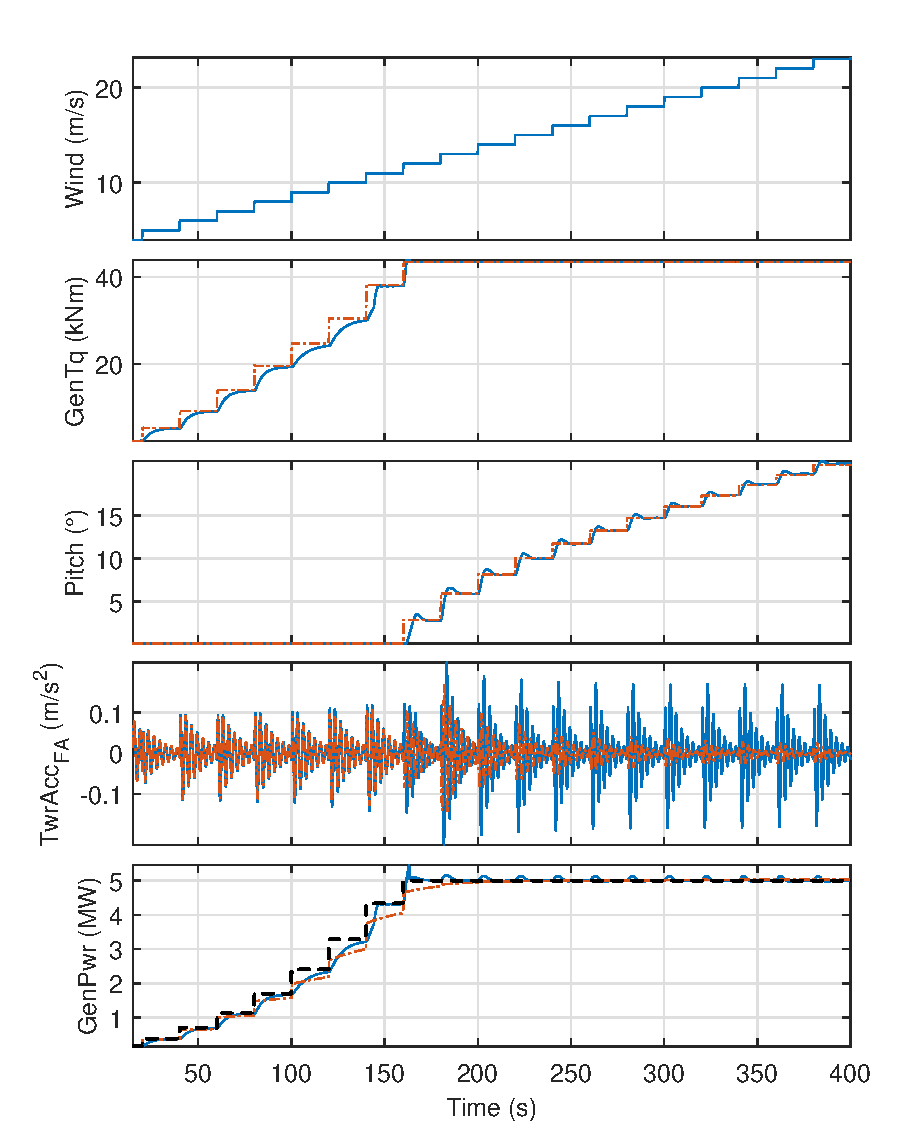
\includegraphics[width=0.495\textwidth, trim={0.cm 0cm 0cm 0.5cm}, clip]{figures/Figures_ADi/cmpCtrlTimeDomain_All_RefSimulinkClosedLoop_beta.eps}}\hfill
    \subfloat[Turbulent wind, mean CPU time MPC 9.88$\cdot 10^{-4}$\,s]{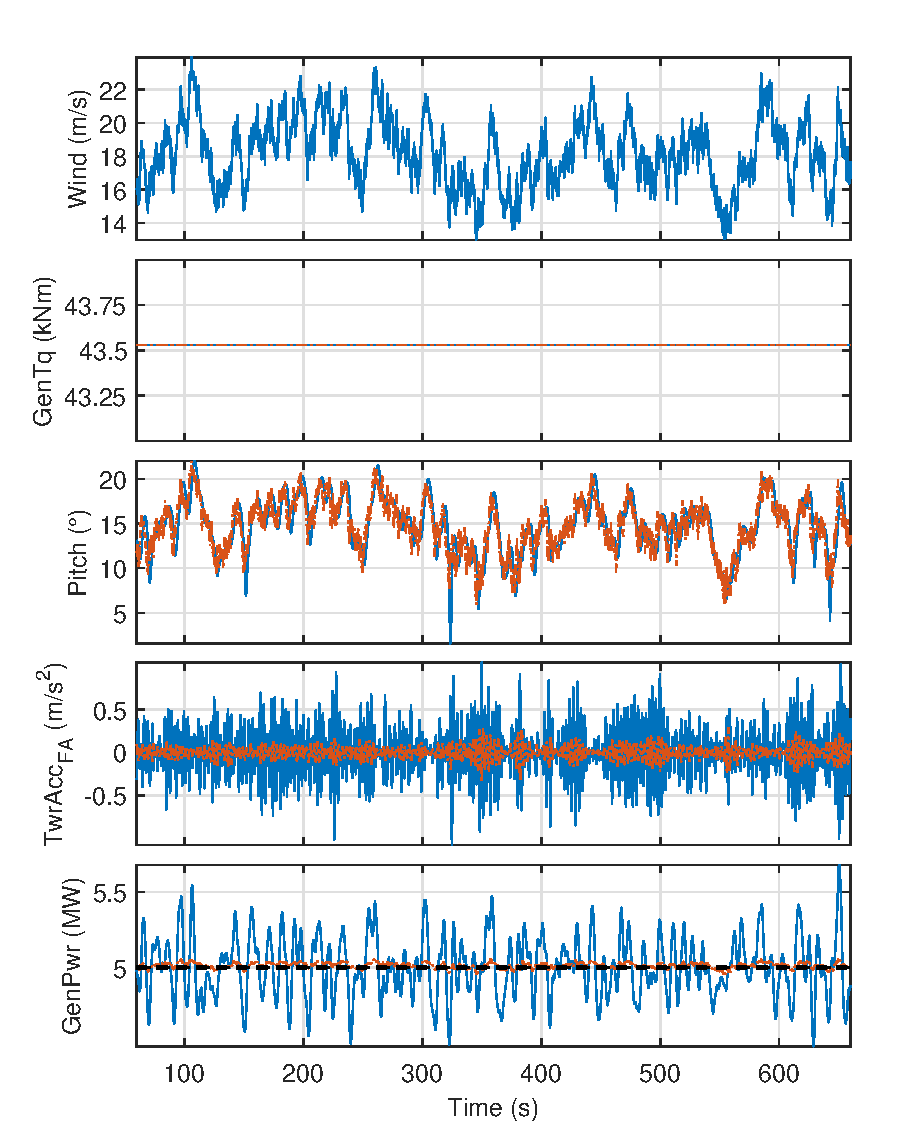
\includegraphics[width=0.495\textwidth,trim={0.cm 0cm 0cm 0.5cm}, clip]{figures/Figures_ADi/cmpCtrlTimeDomain_All_RefSimulinkClosedLoopNTW18_beta.eps}}\hfill
    %\subfloat[blc blc]{\includegraphics[width=0.31\textwidth]{figures/twoTurbinesGreedyOpt_2d.eps}}
    \caption[Controller comparison on qLPV model Mdl2: baseline PI vs.\ qLMPC for stepped wind sweep and turbulent wind.]{Controller comparison on qLPV model Mdl2: baseline PI (\mlBlue) vs.\ qLMPC (\mlOrange) for stepped wind sweep and turbulent wind (18~m/s mean, turbulence class B) with power reference~(\mlBlackDashed). Displayed signals: freestream wind speed, control inputs, tower fore-aft
        accelerations, and power output.}
    \label{fig:CtrlCmpMdlSweep}
\end{figure}
%
In the first test case, the wind speed is increased stepwise from 4\,m/s to 23\,m/s in steps with a duration of 20\,s, resulting in a simulation time of 400\,s, with the first 15\,s discarded as a transient. In the second scenario, 660\,s of turbulent wind with a mean speed of 18\,m/s and turbulence class B of the International Electrotechnical Commission (IEC) is used to assess controller performance under realistic wind conditions, and the first 60\,s are left out of the analysis. The results are shown in Figure~\ref{fig:CtrlCmpMdlSweep}.
%

Figure~\ref{fig:CtrlCmpMdlSweep}(a) shows the controller comparison for the stepped wind sweep covering nearly the entire operating range. In below-rated wind conditions, the two controllers achieve comparable performance. In above-rated wind conditions, however, predictive pitch control considerably reduces tower fore-aft acceleration and power variance. Overall, the standard deviation ratios for the tower fore-aft acceleration and power tracking error are 1.74 and 1.14 (corresponding to variance reduction factors of 3.04 and 1.29), as shown in Table~\ref{tab:ControllerComparisonMerged}.
%
Figure~\ref{fig:CtrlCmpMdlSweep}(b) shows results for the turbulent wind. The improvements over the baseline PI are even more pronounced than in the stepped sweep case. For the tower fore-aft acceleration and power tracking error, the qLMPC yields standard deviation ratios of 4.14 and 11.35 (equivalent to variance reduction factors of 17.14 and 128.88), see Table~\ref{tab:ControllerComparisonMerged}.

The QP is solved using a linear complementarity problem formulation with Lemke's algorithm \cite{cisneros2020velocity}, warm-started with the solution of the previous sample, which enables fast computation, as real-time capability is a critical requirement for online optimization-based control. Of the 50001 controller cycles at a sampling time of 8\,ms needed for the 400\,s simulation time of the stepped wind sweep, only one cycle exceeded the sampling time and only 13 exceeded 2\,ms. The mean CPU time was approximately 1\,ms, as shown in the subplot captions of Figure~\ref{fig:CtrlCmpMdlSweep}. These measurements were obtained in MATLAB R2023a on an Intel Core i7-11850H (2.5\,GHz, 8 cores) running Windows 10. Note that for deployment on a physical turbine, a fallback strategy would be required to handle the rare cases where the solver exceeds the sampling time. This was not implemented in this proof-of-concept, but several options exist, such as blending the last available qLMPC solution with the output of the PI feedback controller.

The improvements regarding the reduction of tower acceleration and power variance come at the price of higher pitch activity. As summarized in Table~\ref{tab:ControllerComparisonMerged}, the standard deviation of the blade pitch rate increases by a factor of approximately 3.6 in the stepped wind sweep and 3.7 in the turbulent wind case, and that of the generator torque rate by a factor of approximately 2.6 in the stepped wind sweep. In the turbulent wind case, both controllers operate at rated generator torque throughout, resulting in zero torque rate standard deviation.

\begin{table}[t]
    \centering
    \caption[Standard deviation comparison with qLPV model Mdl2: Baseline PI vs.\ qLMPC for stepped wind sweep and turbulent wind.]%
    {Standard deviation comparison with qLPV model Mdl2: Baseline PI vs.\ qLMPC for stepped wind sweep and turbulent wind (18\,m/s mean, IEC class B).
        The standard deviations obtained with the PI controller are divided by those obtained with the qLMPC;
        quotients above~1 indicate improvement. Ratios are computed from unrounded values.}
    \label{tab:ControllerComparisonMerged}
    \begin{tabular}{l rr}
        \toprule
        {Standard Deviation of} & {Stepped wind sweep} & {Turbulent wind} \\
        {Signal (unit)} & \multicolumn{2}{c}{std PI / std qLMPC = ratio} \\
        \midrule
        Tower fore-aft acc. (m/s$^2$)  & $0.0597 / 0.0342 \approx 1.74$ & $0.3110 / 0.0751 \approx 4.14$  \\
        Power tracking error (kW)& $176.01 / 154.95 \approx 1.14$ & $201.12 / 17.72 \approx 11.35$  \\
        Generator torque rate (kNm/s)  & $0.56 / 1.47 \approx 0.38$     & $0.00 / 0.00 = {-}$     \\
        Blade pitch rate (\textdegree/s)  & $0.21 / 0.76 \approx 0.28$     & $1.21 / 4.44 \approx 0.27$   \\
        \bottomrule
    \end{tabular}
\end{table}

As more improvement in power variance was observed for the above-rated turbulent wind, the following discussion focuses on this case. In the results above, the pitch command increments are penalized, but the pitch rate state is not, and the pitch rate limit of 13\textdegree/s is relatively high compared to the 8\textdegree/s of the NREL 5MW reference turbine \cite{jonkman2009definition}. Figure~\ref{fig:CtrlCmpRates} shows the results of six test runs with different pitch rate limits on the plant without the wind filters: three with the baseline PI controller and three with the qLMPC algorithm.
\begin{figure}[h]
    \subfloat[Baseline PI controller]{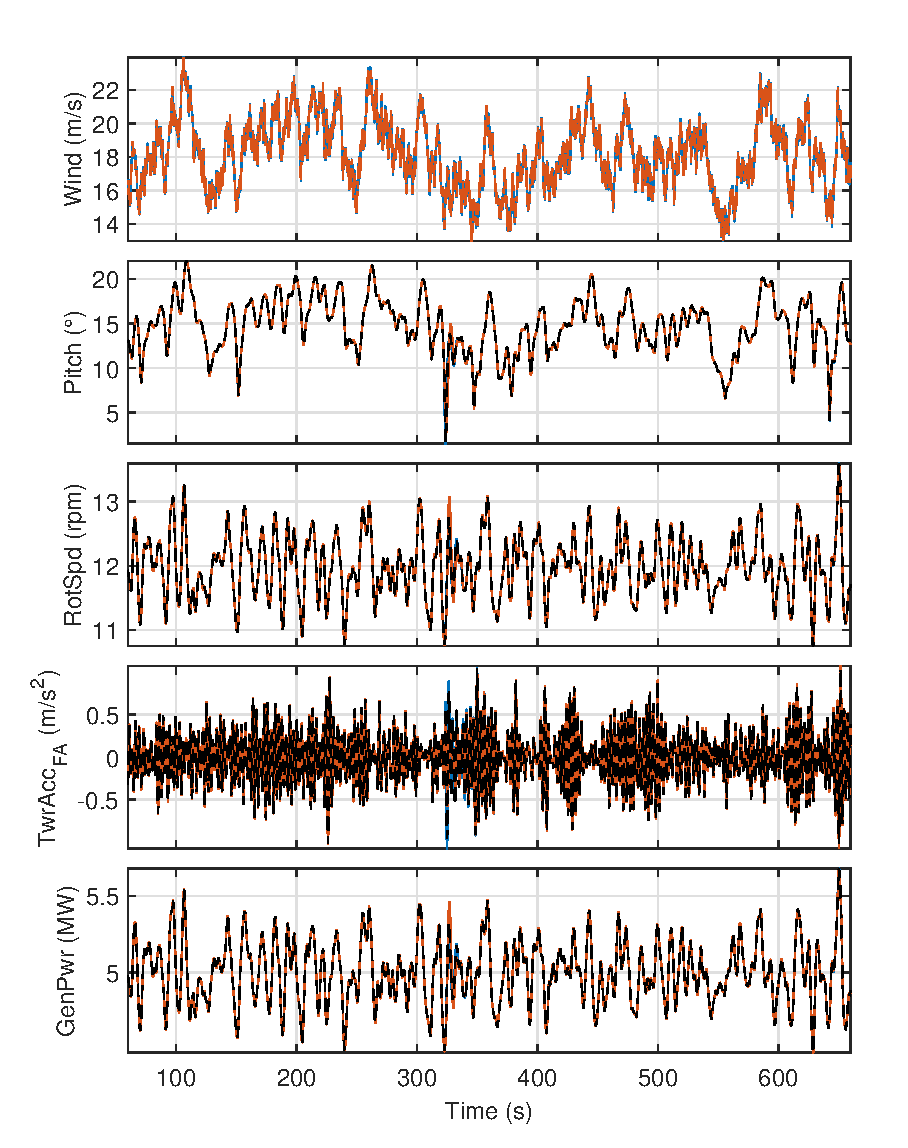
\includegraphics[width=0.495\textwidth,trim={0.cm 0cm 0cm 0.65cm}, clip]{figures/figDirConstr1/cmpTimeDomain_All5PINewLim_NoFilt.eps}}\hfill
    \subfloat[qLMPC algorithm]{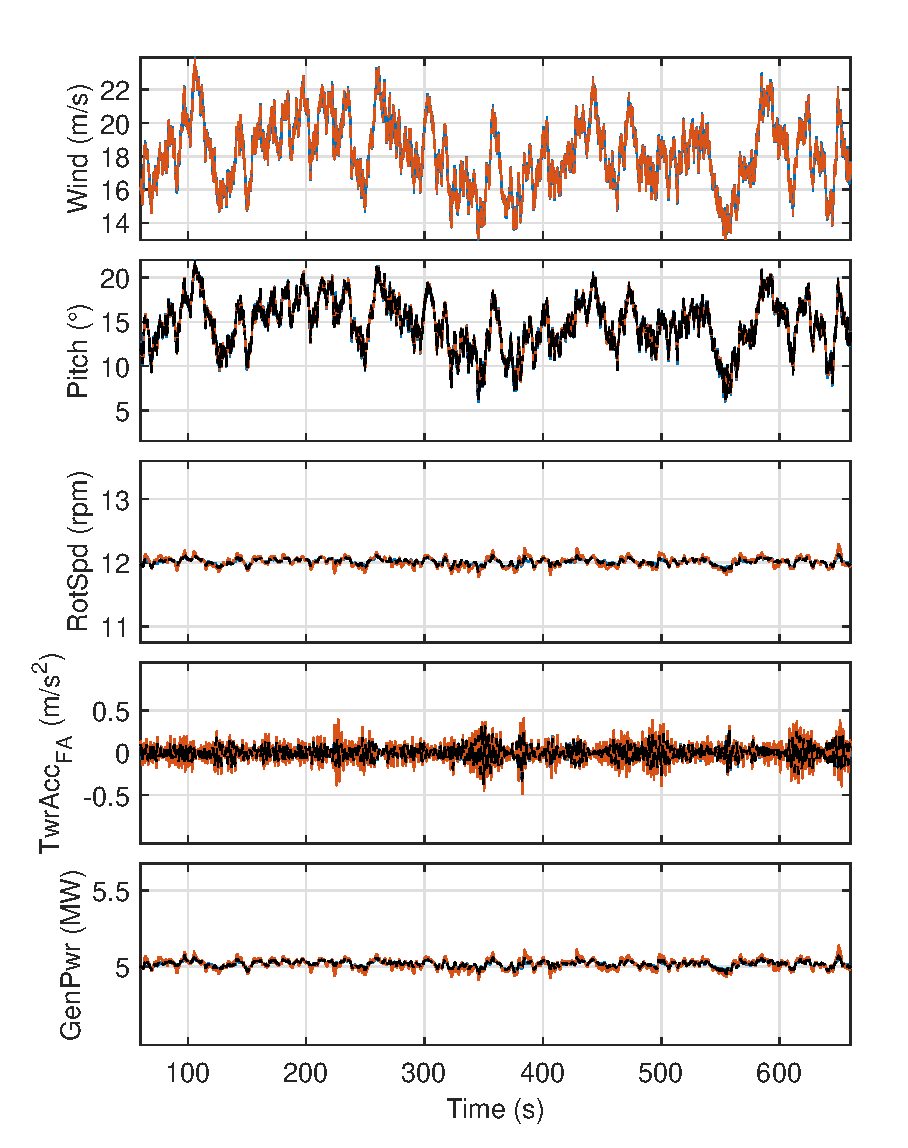
\includegraphics[width=0.495\textwidth,trim={0.cm 0cm 0cm 0.65cm}, clip]{figures/figDirConstr1/cmpTimeDomain_All5MPCNewLim.eps}}\hfill
    \caption[Controller comparison on qLPV model Mdl2: baseline PI and qLMPC with different pitch rate limits.]{Controller comparison on qLPV model Mdl2: baseline PI and qLMPC with different pitch rate limits for turbulent wind (18\,m/s mean, turbulence  class B), both controllers on the plant without the wind filters. Rate limits: Standard 8\textdegree/s~(\mBlack), high 13\textdegree/s~(\mlBlue), and low 4\textdegree/s~(\mlOrange). Displayed signals: freestream wind speed, pitch, states, and power.}
    \label{fig:CtrlCmpRates}
\end{figure}
The effect of different pitch rate limits on the PI controller is depicted in Figure~\ref{fig:CtrlCmpRates}(a), and on the qLMPC design in Figure~\ref{fig:CtrlCmpRates}(b). The selected pitch rate limits of 4\textdegree/s, 8\textdegree/s, and 13\textdegree/s represent a range from conservative to highly responsive actuator capabilities. They were chosen to explore both realistic hardware limitations and the potential performance gains of faster actuation. The signals shown for both control algorithms are the wind speed, collective blade pitch angle, rotor speed, fore-aft tower acceleration, and generator power. The generator torque does not change in this above-rated test case and is hence not shown. Under baseline PI control, the pitch rate limit has almost no effect: the standard deviations of the tower fore-aft acceleration, the rotor speed and the power tracking error change by at most about 1\,\% between 4\textdegree/s and 13\textdegree/s. The PI controller reaches the respective rate limit only occasionally and exceeds 4\textdegree/s during less than 1\,\% of the time, as the rotor acts as a filter in this pure feedback design. In contrast, the qLMPC exceeds 4\textdegree/s during more than a third of the time if allowed, and shows a considerable difference between the 4\textdegree/s rate limit and the two higher rates. Allowing a pitch rate of 8\textdegree/s or faster improves rotor speed regulation and reduces the standard deviations of rotor speed and power by a factor of about 1.6 compared to the 4\textdegree/s limit. However, it also leads to higher pitch activity. The qLMPC reduces the variance of rotor speed, tower fore-aft movement, and power output compared to the PI controller for all rate limits, even at a 4\textdegree/s rate limit, where the standard deviations of the tower fore-aft acceleration and of the power tracking error are still reduced by factors of 2.58 and 6.42. The qLMPC benefits from higher pitch rates, as a faster pitch response enables better disturbance rejection, e.g.\ of gusts. The trade-off between actuator activity on the one hand and load reduction and smoother power output on the other is a design decision, which may also vary over the turbine's lifetime as the pitch bearings age. 
%
Figure~\ref{fig:CtrlCmpFilt2} shows both controllers on the plant with the wind filters introduced in Section~\ref{sec:qLPVModelVerificationwithFAST0}, which imitate the averaging effect of a wind field acting on the whole rotor instead of a single-point wind speed. 
\begin{figure}[h]
    \centering
    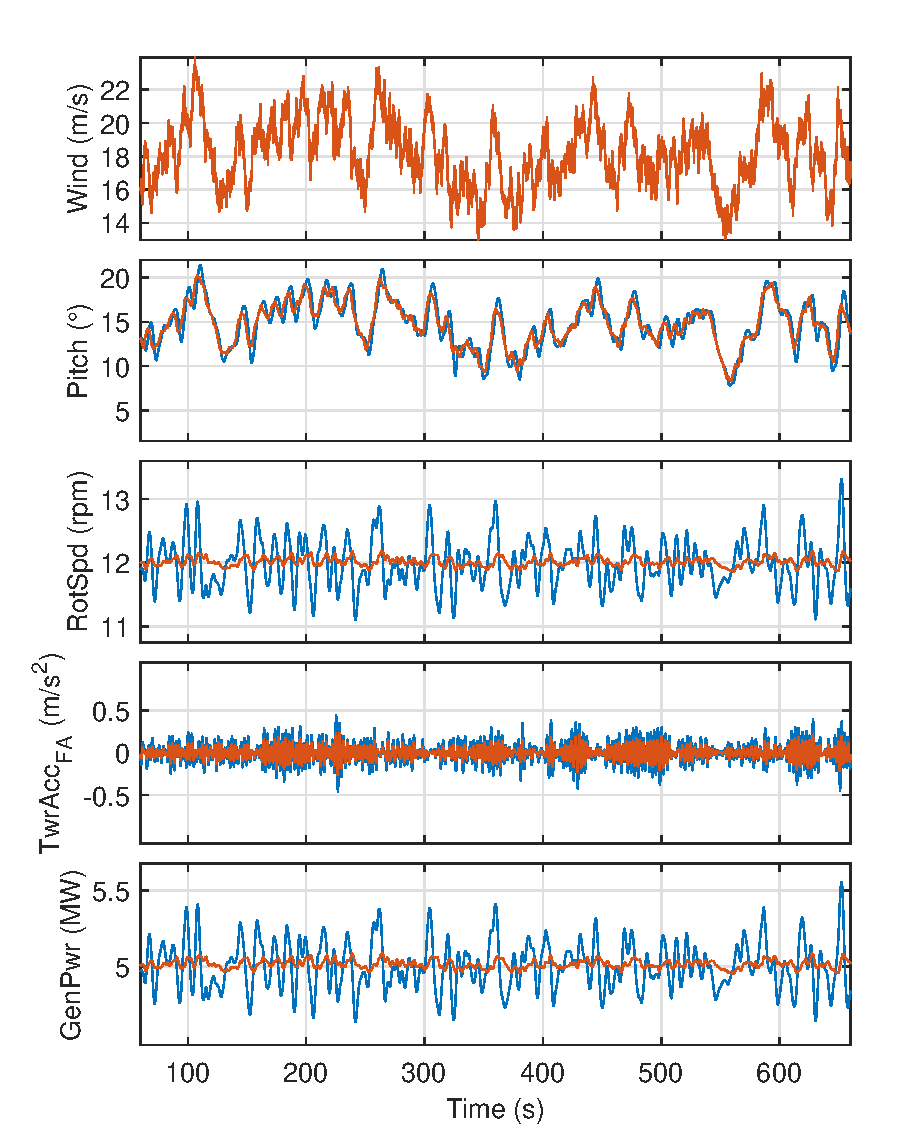
\includegraphics[width=0.495\textwidth,trim={0.cm 0cm 0cm 0.7cm}, clip]{figures/figDirConstr1/cmpTimeDomain_All5PIvsMPC_Filt.eps}
    \caption[Controller comparison on qLPV model Mdl2 with filtered wind: baseline PI and qLMPC.]{Controller comparison on qLPV model Mdl2 with filtered wind: baseline PI (\mlBlue) and qLMPC (\mlOrange), qLMPC and Mdl2 with rotor-effective wind filters for turbulent wind (18\,m/s mean, turbulence class B), pitch rate limit 13\textdegree/s. Displayed signals: freestream wind speed, pitch, states, and power.}
    \label{fig:CtrlCmpFilt2}
\end{figure}
The standard deviations of the pitch derivative, the rotor speed, the tower fore-aft acceleration and the power tracking error for Figures~\ref{fig:CtrlCmpRates} and~\ref{fig:CtrlCmpFilt2} are summarized in Table~\ref{tab:stddev_unified}.

\begin{table}[htbp]
    \centering
    \setlength{\tabcolsep}{4.5pt}
    \caption[Standard deviations: Baseline PI and qLMPC for turbulent wind and different pitch rate limits.]%
    {Standard deviations: Baseline PI and qLMPC for turbulent wind and different pitch rate limits
        (\textdegree/s). Columns 4, 8, 13: plant without rotor-effective wind filters. Last column: plant
        with filters, qLMPC scheduled with the filtered wind. Brackets: PI value at 8\textdegree/s without
        filters divided by the entry; for the filtered qLMPC, the filtered PI value is used instead.}
    \label{tab:stddev_unified}
    \begin{tabular}{ll rrrr}
        \toprule
        & & \multicolumn{4}{c}{Rate limit (\textdegree/s)} \\
        \cmidrule(lr){3-6}
        %Ctrl. & Signal & 4 & 8 & 13 & 13, filt. \\
        Ctrl. & Signal & low: 4 & standard: 8 & high: 13 & filt. wind: 13 \\
        \midrule
        \multirow{4}{*}{PI}
        & Tower acc.\ (m/s$^2$)      & 0.3076 (1.01) & 0.3108 (1.00) & 0.3110 (1.00) & 0.1300 (2.39) \\
        & Power error (kW)           & 202.04 (1.00) & 201.22 (1.00) & 201.12 (1.00) & 159.33 (1.26) \\
        & Rotor speed (rpm)          & 0.4830 (1.00) & 0.4810 (1.00) & 0.4808 (1.00) & 0.3812 (1.26) \\
        & Pitch rate (\textdegree/s) & 1.13 (1.04)   & 1.18 (1.00)   & 1.21 (0.98)   & 0.71 (1.66) \\
        \midrule
        \multirow{4}{*}{qLMPC}
        & Tower acc.\ (m/s$^2$)      & 0.1204 (2.58) & 0.0813 (3.82)  & 0.0751 (4.14)  & 0.0723 (1.80) \\
        & Power error (kW)           & 31.35 (6.42)  & 19.56 (10.29)  & 17.72 (11.35)  & 27.40 (5.82) \\
        & Rotor speed (rpm)          & 0.0743 (6.47) & 0.0464 (10.37) & 0.0422 (11.40) & 0.0655 (5.82) \\
        & Pitch rate (\textdegree/s) & 2.91 (0.41)   & 4.07 (0.29)    & 4.44 (0.27)    & 0.54 (1.31) \\
        \bottomrule
    \end{tabular}
\end{table}

The same axis limits as in Figure~\ref{fig:CtrlCmpRates}(a) are used in Figure~\ref{fig:CtrlCmpRates}(b) to highlight the improvements possible with the qLMPC and in Figure~\ref{fig:CtrlCmpFilt2} to visualize the smoothing effect of the filters on both PI and qLMPC. On the filtered plant, the largest pitch rate is 2.5\textdegree/s for the PI controller and 2.6\textdegree/s for the qLMPC, although the pitch rate limit is 13\textdegree/s, so all rate limits from 3\textdegree/s upwards are inactive and give identical results. The filters alone reduce the standard deviations of the PI controller by a factor of 2.39 for the tower fore-aft acceleration and 1.26 for the rotor speed and the power tracking error. On the filtered plant, the qLMPC still reduces the standard deviations of the tower fore-aft acceleration, the rotor speed and the power tracking error by factors of 1.80, 5.82 and 5.82 compared with the PI controller, but considerably less than without the filters. At the same time, the pitch activity changes fundamentally: with the filtered wind, the standard deviation of the qLMPC pitch rate is 0.54\textdegree/s, which is even below the 0.71\textdegree/s of the PI controller, whereas without the filters the qLMPC requires 4.44\textdegree/s, more than three times as much as the PI controller. A large part of both the pitch activity and the improvement of the qLMPC without the filters is therefore caused by the high-frequency fluctuations of the single-point wind speed. These fluctuations excite the plant strongly, so that the PI controller, which only reacts to the resulting rotor speed changes, leads to large oscillations, while the qLMPC, which knows the wind speed exactly, compensates them with fast pitch action. A real rotor averages these fluctuations out. The unfiltered case nevertheless shows the benefit of high pitch rates for fast disturbances and represents a worst case regarding the demanded pitch activity.
%
All ratios in this table relate the two controllers on the same plant, with one exception: the last column of the PI block relates the PI on the plant with the wind filters to the PI on the plant without the filters and thus shows the effect of the filters themselves.

\subsubsection{Results on FAST}\label{subsubsec:qLMPCFASTresults}

Figure~\ref{fig:CtrlCmpFAST} shows the baseline PI controller, the original qLMPC, and the notch filter and smooth designs of Section~\ref{sec:qLMPCFAST} on FAST for the stepped wind sweep and the turbulent 18\,m/s wind field of Section~\ref{quasiLPVMPCResults}, with a pitch rate limit of 13\textdegree/s. The standard deviations are summarized in Table~\ref{tab:CtrlComparisonFAST}, with the ratio of the baseline PI value to the value of the respective controller in parentheses.
%
\begin{figure}[htbp]
    \subfloat[Stepped wind sweep.]{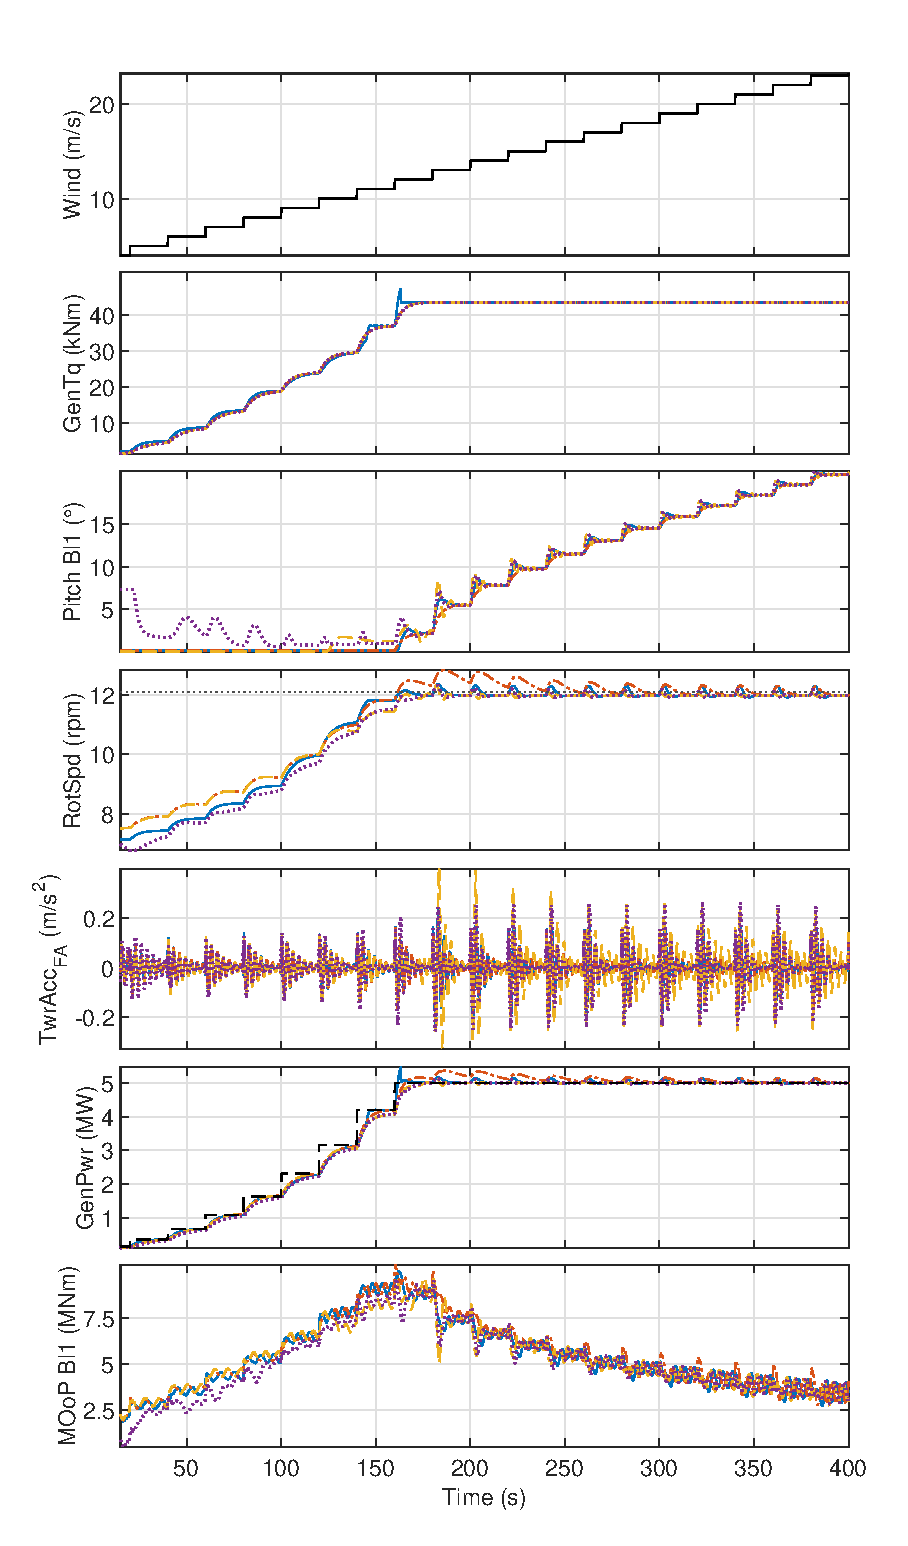
\includegraphics[width=0.495\textwidth,trim={0.cm 0cm 0cm 0.9cm}, clip]{figures/figDirFASTthesis/cmpCtrlFASTthesis_Sweep_PI_beta_flapNotch_flapNotchSmooth12.eps}}\hfill
    \subfloat[Turbulent wind, 18~m/s mean, turbulence class~B.]{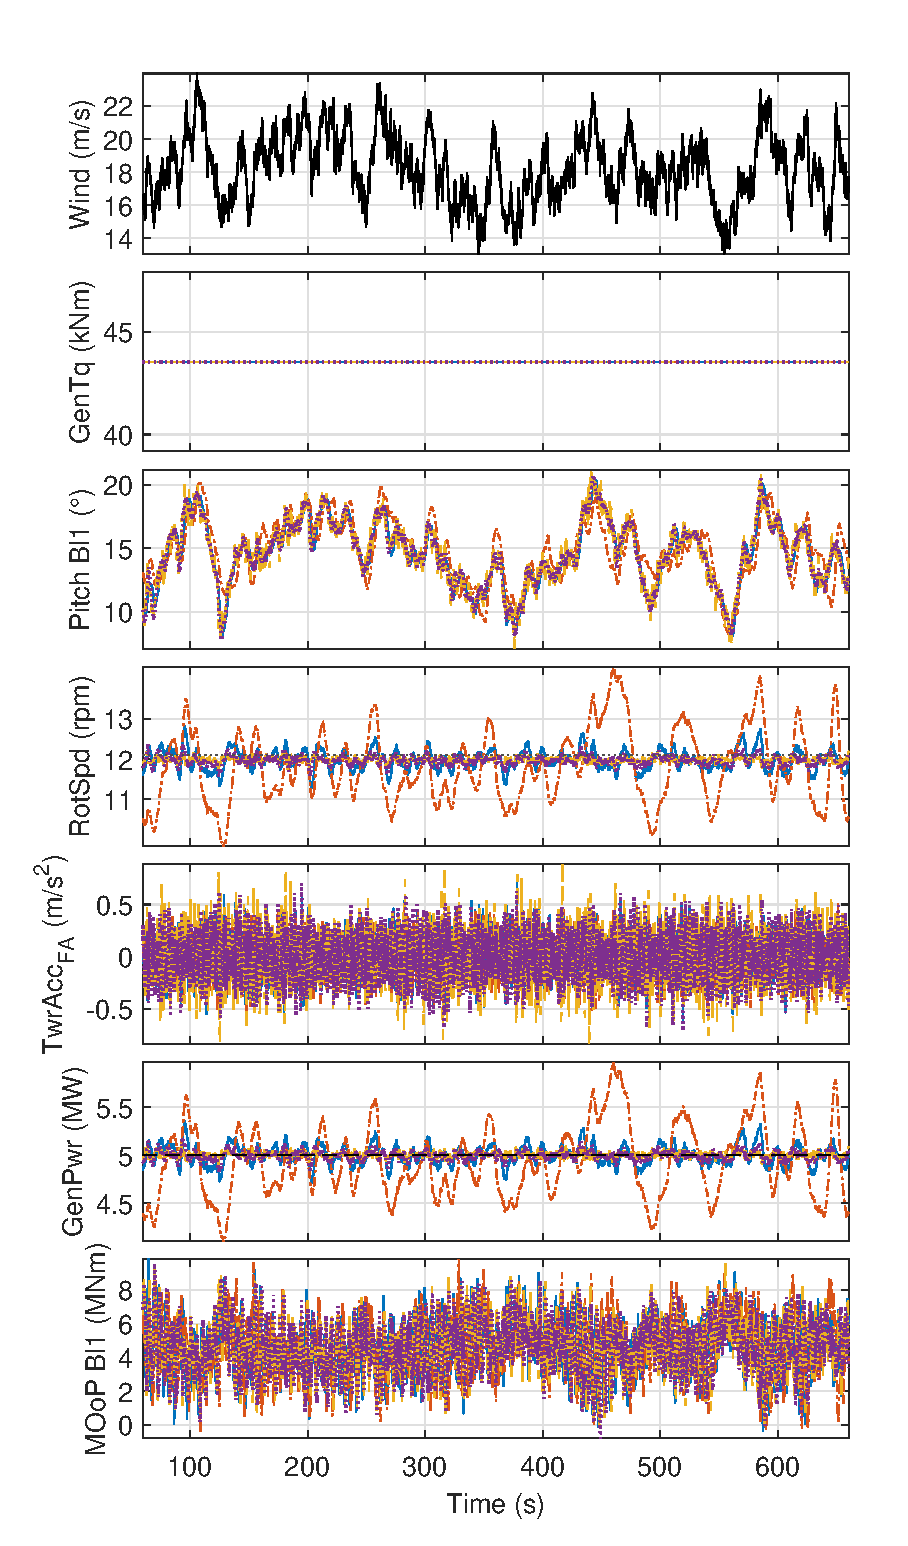
\includegraphics[width=0.495\textwidth, trim={0.cm 0cm 0cm 0.9cm}, clip]{figures/figDirFASTthesis/cmpCtrlFASTthesis_NTM18B_PI_beta_flapNotch_flapNotchSmooth12.eps}}
    \caption[Controller comparison on FAST: baseline PI, original qLMPC, and the qLMPC designs for FAST]{Controller comparison on FAST: baseline PI controller (\mlBlue), original qLMPC (\mlOrange), notch filter design (\mlYellow), and smooth design (\mlPurple) for the stepped wind sweep and turbulent wind (18\,m/s mean, turbulence class B), pitch rate limit 13\textdegree/s. Displayed signals: freestream wind speed, generator torque, blade 1 pitch angle, rotor speed, tower fore-aft acceleration, generator power with its reference (black dashed line), and blade 1 root out-of-plane moment.}
    \label{fig:CtrlCmpFAST}
\end{figure}
In the stepped wind sweep, shown in Figure~\ref{fig:CtrlCmpFAST}(a), the differences between the controllers are small. The original qLMPC, depicted in orange, slightly outperforms the baseline PI controller, shown in blue, with a decrease of 8\% in the standard deviation of the tower fore-aft acceleration and of 4\% in those of the power tracking error and the rotor speed. This is achieved with smoother pitching, so that all four values show an improvement. The two other qLMPC designs, which were developed to address the issues in turbulent wind, show no overall improvement for the stepped wind sweep. Only the standard deviation of the rotor speed of the notch filter design decreases slightly, but due to the much more aggressive pitching, this does not translate into a lower standard deviation of the power tracking error. Presumably, these performance decreases result from the rotor-effective wind filter, which delays the scheduling wind speed although the wind steps act on the whole rotor area at once. This is particularly noticeable for the smooth design, whose pitch angle deviates from zero below rated wind speed.

In the turbulent wind, the original qLMPC, which performs very well on Mdl2 for both test cases and reasonably well on FAST for the stepped wind sweep test case, fails on FAST: the rotor speed varies between 10\,rpm and 14.3\,rpm, and the standard deviations of the rotor speed and of the power tracking error are 3.7 and 3.6 times those of the baseline PI controller. The notch filter design reduces these standard deviations by factors of 3.8 and 3.3 compared with the baseline PI controller, and the smooth design by factors of 2.1 and 2.0. This is less than the factor of 11.4 on Mdl2 (Table~\ref{tab:stddev_unified}), but still a considerable smoothing of the power output. In contrast to Mdl2, however, the tower fore-aft acceleration is not reduced but increased, by 35\% for the notch filter design and 16\% for the smooth design, and the tower base DEL increases by 27\% and 12\%; for the wind of the second verification set and a pitch rate limit of 8\textdegree/s, the increases are 33\% and 16\%, see Section~\ref{subsec:ComparisonWindTurbineControlDesigns}. The pitch rate standard deviation is 5.9 times that of the baseline PI controller for the notch filter design and 2.4 times for the smooth design. The adaptations thus make the qLMPC applicable to FAST and retain a large part of the power smoothing in turbulent wind, but not the reduction of the tower loads achieved on Mdl2. The smooth design trades part of the power smoothing for considerably less pitch activity and a smaller increase of the tower loads.

\begin{table}[h]
    \centering
    \caption[Controller comparison on FAST for stepped wind sweep and turbulent wind.]{Controller comparison on FAST v8.16 for the stepped wind sweep and turbulent wind (18\,m/s mean, turbulence class B), pitch rate limit 13\textdegree/s: standard deviations of the tower fore-aft acceleration, the power tracking error, the rotor speed, and the (collective) pitch rate. In parentheses the ratio baseline PI/controller; values above 1 indicate an improvement.}
    \label{tab:CtrlComparisonFAST}
    \begin{tabular}{ll rrrr}
        \toprule
        & & & \multicolumn{3}{c}{qLMPC} \\
        \cmidrule(lr){4-6}
        Wind & Signal & Baseline PI & original & notch filter & smooth \\
        \midrule
        \multirow{4}{*}{Sweep}
        & Tower acc.\ (m/s$^2$)      & 0.0558 & 0.0516 (1.08) & 0.0826 (0.67) & 0.0684 (0.82) \\
        & Power error (kW)           & 141.85 & 136.15 (1.04) & 144.65 (0.98) & 156.66 (0.91) \\
        & Rotor speed (rpm)          & 1.6977 & 1.6264 (1.04) & 1.4993 (1.13) & 1.7719 (0.96) \\
        & Pitch rate (\textdegree/s) & 0.22   & 0.12 (1.76)   & 0.50 (0.44)   & 0.39 (0.55) \\
        \midrule
        \multirow{4}{*}{Turbulent}
        & Tower acc.\ (m/s$^2$)      & 0.1712 & 0.1689 (1.01) & 0.2310 (0.74) & 0.1990 (0.86) \\
        & Power error (kW)           & 59.60  & 214.42 (0.28) & 17.90 (3.33)  & 29.18 (2.04) \\
        & Rotor speed (rpm)          & 0.2460 & 0.9035 (0.27) & 0.0653 (3.77) & 0.1145 (2.15) \\
        & Pitch rate (\textdegree/s) & 0.49   & 0.68 (0.72)   & 2.87 (0.17)   & 1.18 (0.41) \\
        \bottomrule
    \end{tabular}
\end{table}

%\input{figures/figDirFASTthesis/resultsFASTthesis_NTM18B_PI_beta_flapNotch_flapNotchSmooth12}

The application of the proposed velocity-based qLMPC concept to the qLPV model considerably reduces tower movements and power output fluctuations. As noted at the start of this section, DEL reduction is not directly a qLMPC objective. On FAST, with the adaptations of Section~\ref{sec:qLMPCFAST}, the qLMPC still reduces the power fluctuations, but the tower loads increase, as shown above and in the comparison with the other controllers in Section~\ref{subsec:ComparisonWindTurbineControlDesigns}.

This study shows that considerable performance improvements are possible without model mismatch, and this best-case scenario underlines the potential of the algorithm. However, even the model mismatch between the carefully tuned qLPV model and FAST deteriorates the performance of the original qLMPC. With the adaptations for FAST, a large part of the power smoothing is retained, but the tower loads increase, which shows the sensitivity of the qLMPC to model mismatch. Moreover, the performance improvement comes at the cost of requiring accurate wind information, obtained either through expensive sensors such as lidars or through wind speed estimation. A purely feedback-based improvement over standard collective pitch control is individual pitch control, which uses blade root moments and the rotor azimuth position as additional feedback signals and is already widely deployed in commercial turbines. This approach has been extensively investigated in both theoretical studies and field tests and has proven to be an effective strategy to further reduce mechanical loads, either as an alternative or in addition to MPC. While its primary focus is on reducing blade loads, a slight reduction in tower loads is also possible, as will be discussed in the next section.

\section{Individual Pitch Control Design and Application}\label{section:Individal Pitch PI Control} 
IPC is a control technique designed to mitigate cyclic loads on wind turbine blades by independently adjusting the pitch angle of each blade. These cyclic loads primarily result from wind shear, i.e., the increase in wind speed with altitude due to reduced surface friction farther from the ground. Additional causes of load imbalances include yaw misalignment, rotor tilt, turbulence, gusts, and tower shadow effects. These effects lead to asymmetric aerodynamic loading, which induces bending moments perpendicular to the rotor plane at the blade roots, referred to as out-of-plane bending moments. They occur at specific multiples of the rotor's rotational frequency, commonly referred to as $n\text{P}$ frequencies, e.g., $1\text{P}$ and $2\text{P}$ correspond to once and twice per revolution, respectively. These periodic loads accumulate fatigue damage in the blades and, via the resulting tilt and yaw moments, in the hub, shaft and nacelle. In addition, they can excite the turbine's natural structural modes if an $n\text{P}$ frequency coincides with a natural frequency, which further accelerates fatigue and reduces component lifespan.

The turbine blade deformation can be decomposed into three primary directions relative to the blade itself: flapwise, which is perpendicular to the rotor plane if the blade is not pitched, edgewise within the rotor plane, and torsional twisting along the blade's axis. The flapwise and edgewise blade root bending moments are measured directly, for example via strain gauges, and transformed into moments within and perpendicular to the rotor plane using the current pitch angle. The out-of-plane moments serve as feedback for IPC. IPC suppresses these loads by transforming the blade root moments from the rotating into the non-rotating coordinate system, computing tilt and yaw pitch demands with a controller, and transforming these back into the rotating frame before adding them to the blade pitch signals.

The block diagram in Figure~\ref{fig:BlockIPC} illustrates the IPC architecture. It shows the main components of the system, including the controller, which is divided into the power controller and the IPC controller, highlighted in red. The figure also displays the NREL 5MW wind turbine, the pitch actuator, and the torque actuator.
\begin{figure}[ht]
    \centering
    \includegraphics[width=0.9\textwidth,trim={0 0cm 0cm 0.005cm},clip]{figures/Figures_ADi/turbineCtrlBetaIPCcl.pdf}
    \caption[Block diagram of IPC enhancing baseline power control.]{Block diagram of IPC enhancing baseline power control: the power control sets the collective pitch and generator torque references. In the IPC block (red), MBC transforms the blade root moments $M_{yci}$ into the tilt and yaw moments $M_c$ and $M_s$, which are scaled with $k_M$ and the PI gains $K_{\text{IPC}}$. Its outputs are transformed back into individual pitch demands $\beta_{i,\text{IPC}}$ added to $\beta_{0,\text{ref}}$.}
    \label{fig:BlockIPC}
\end{figure}
%
In this work, PI controllers are utilized rather than full PID architectures. This choice is consistent with the NREL 5MW baseline controller provided in FAST. Furthermore, a joint optimization including a derivative gain, see Section~\ref{subsection: IPCOptCriteria}, reduced the blade DEL by only 2.3 percentage points more, at almost twice the pitch activity, which would increase actuator wear.

The three blade pitch angles $\beta_1$, $\beta_2$, and $\beta_3$ are the outputs of the pitch actuators corresponding to the references $\beta_{1,\text{ref}}$, $\beta_{2,\text{ref}}$, and $\beta_{3,\text{ref}}$. These references are the sum of the collective reference signal $\beta_{0,\text{ref}}$ from the power controller and the respective IPC adjustments $\beta_{1,\text{IPC}}$, $\beta_{2,\text{IPC}}$, and $\beta_{3,\text{IPC}}$.
%
As before, the power control loop sets the collective pitch reference $\beta_{0,\text{ref}}$ as well as the generator torque reference $T_{g,\text{ref}}$, based on feedback from the generator speed $\omega_g$.
%
The IPC adjustments are derived from the out-of-plane blade root bending moments $M_{yc1}$, $M_{yc2}$, and $M_{yc3}$ and the position of the first blade $\theta_{r}$, also called the rotor position or rotor azimuth. The blade root moments are transformed from the rotating into the non-rotating coordinate system by a multiplication with the matrix $\frac{2}{3}V_{\theta_{r}}^{T}$. The back-transformation before applying the control signals to the rotating blades is done by a multiplication with the matrix $V_{\theta_{r}}$. The underlying method for these coordinate transformations, known as multiblade coordinate transformation, and the design of $V_{\theta_{r}}$ are explained in detail below.

% (\texttt{RootMyb1} and \texttt{RootMyc1} for the first blade)

\subsection{Multiblade Coordinate Transformation} \label{sec:MBC}
Multiblade coordinate transformation (MBC) enables the conversion of dynamic loads from the rotating coordinate system, defined by the azimuth angle $\theta_{r}$, to a fixed tower coordinate system. Specifically, load components at the rotation frequency are transformed via the MBC to quasi-static loads. Hence, MBC allows for a more accurate assessment of the loads acting on the turbine tower and other non-rotating components. 

Note that the blade root moments measured by strain gauges are expressed in the blade coordinate system, which rotates with the pitch angle: the flapwise moment $M_{ybi}$ acts perpendicular to the chord line and the edgewise moment $M_{xbi}$ along it. For IPC, the moments perpendicular to the rotor plane are required. These out-of-plane moments $M_{yci}$ are obtained by rotating the flapwise and edgewise moments by the pitch angle $\beta_i$ of the respective blade into the coned coordinate system, which does not rotate with the pitch \cite{jonkman2005fast}:
\begin{equation} \label{eq:MoopFAST}
    M_{yci} = M_{ybi} \cos(\beta_i) - M_{xbi} \sin(\beta_i), \quad i = 1, 2, 3.
\end{equation}
For zero pitch, the out-of-plane moment thus equals the flapwise moment, while with increasing pitch angle, an increasing part of the edgewise moment contributes to the out-of-plane moment. FAST provides both the moments in the blade coordinate system and the out-of-plane moments in the coned coordinate system as outputs. For convenience, the out-of-plane moments $M_{yci}$ provided by FAST are used directly as feedback signals for IPC in this work.

Applying MBC to convert the rotating blade root out-of-plane moments into a fixed coordinate system for a three-bladed wind turbine results in the matrix notation 

\begin{equation} \label{eq:MBC}
    \left[ \begin{array}{c}
        M_0\\
        M_c\\
        M_s
    \end{array} \right] = \frac{2}{3}
    \left[ \begin{array}{ccc}
        1/2 & 1/2 & 1/2\\
        \cos(\theta_{r}) & \cos(\theta_{r} + \frac{2\pi}{3}) & \cos(\theta_{r} + \frac{4\pi}{3})\\
        \sin(\theta_{r}) & \sin(\theta_{r} + \frac{2\pi}{3}) & \sin(\theta_{r} + \frac{4\pi}{3})
    \end{array} \right]
    \left[ \begin{array}{c}
        M_{yc1}\\
        M_{yc2}\\
        M_{yc3}
    \end{array} \right], 
\end{equation}
with $M_{yci}$ as the out-of-plane root moment of the $i$-th blade as inputs and the moments in the non-rotating system as outputs, with these moments being the symmetric load moment $M_0$, tilt moment $M_c$ and yaw moment $M_s$, as visualized in Figure~\ref{fig:BlockIPC}. The tilt and yaw moments are used to calculate two cyclic control signals $q_c$ and $q_s$, i.e., $\beta_c$ and $\beta_s$ for IPC. 
The control signal $q_i$ of the $i$-th blade is calculated via the second and third columns of the inverse MBC transformation, i.e., the inverse of the matrix from Equation~\eqref{eq:MBC} %, is then used to calculate 
\begin{equation} \label{eq:inverseMBC}
    \left[ \begin{array}{c}
        q_1\\
        q_2\\
        q_3
    \end{array} \right] = 
    \underbrace{\left[ \begin{array}{ccc}
            \cos(\theta_{r}) &  \sin(\theta_{r})\\
            \cos(\theta_{r} + \frac{2\pi}{3}) &  \sin(\theta_{r} + \frac{2\pi}{3})\\
            \cos(\theta_{r} + \frac{4\pi}{3}) &  \sin(\theta_{r} + \frac{4\pi}{3})
        \end{array} \right]}_{V_{\theta_{r}}}
    \left[ \begin{array}{c}
        q_c\\
        q_s
    \end{array} \right],
\end{equation}
where the signal $q_i$ denotes $\beta_{i,\text{IPC}}$ in IPC for the $i$-th blade. %In Section~\ref{sec:CombinedIPC-TrailingEdgeFlapControl} the same matrix multiplication is once again applied to the $i$-th flap.
Note that the transpose of the matrix $V_{\theta_{r}}$ from Equation~\eqref{eq:inverseMBC}, multiplied by $2/3$, is equal to the last two rows of the MBC matrix, see also \cite{ossmann2017load}. In the context of this work, and as is common in related literature, see, e.g.,~\cite{he2018combined}, the tilt and yaw moments $M_c$ and $M_s$ are controlled via $q_c$ and $q_s$ independently, i.e., any remaining coupling following the MBC transformation between $q_c$ and $M_s$ as well as $q_s$ and $M_c$ is neglected. As the wind turbine dynamics can be approximated as a Linear Time-Invariant (LTI) system after transforming rotor blade dynamics into a fixed coordinate system, using MBC from Equation~\eqref{eq:MBC}, a simple, intuitive control approach is adopted. Two separate SISO controllers, one for the tilt and one for the yaw moment, are designed to reduce the transformed moments $M_c$ and $M_s$. In this work, the same controller parameters are used, resulting in two parameters to be tuned for this PI controller. Note that the moment $M_0$, the collective out-of-plane moment caused by the rotor thrust, is determined by the collective pitch angle set by the baseline power controller and is not used in the IPC controls.

\subsection{IPC Parameter Optimization} \label{subsection: IPCOptCriteria}
The primary objective of wind turbine control is to minimize the Levelized Cost of Energy (LCoE) by balancing the conflicting goals of maximizing power output while minimizing mechanical loads, particularly DELs on the tower and blades. This work leverages controller optimization criteria similar to the ones originally used by \cite{hoffmann2018load}, where a standard baseline wind turbine controller, comprising a generator torque and a CPC PI pitch controller, is augmented with an IPC PI pitch controller and tower damping. The optimization criteria in a multi-objective optimization were the minimization of blade and tower DELs, actuator activity, power tracking error, and the standard deviation of the generated power. However, as in \cite{dittmer2024combined}, only the minimization of the blade DEL is implemented in this work, and the other criteria are used as evaluation criteria. In the following study, the optimization and simulation environment presented in \cite{dittmer2024combined} was used, which uses OpenFAST~v3.2.1. As before, this software is referred to as FAST.
%
The IPC PI controller optimization presented in this thesis consists of two optimization steps for each pitch rate limit:
\begin{enumerate}
    \item In the first step, the proportional and integral gains of the IPC are optimized with the Nelder-Mead simplex algorithm implemented in MATLAB's \textit{fminsearch.m} to reduce the blade DEL. A joint optimization including the derivative gain, tried for a pitch rate limit of 8\textdegree/s, resulted in $K_{\text{D,IPC}} = 0.15$ and a blade DEL reduction 2.3 percentage points higher, but almost twice the pitch activity; therefore only PI controllers are used.
    \item In the second step, the sequential quadratic programming algorithm of MATLAB's \textit{fmincon.m} is started from this result and minimizes the same cost function subject to the constraint that the tower base DEL must not exceed the value obtained with the baseline controller only, i.e., without IPC, at the same pitch rate limit.
\end{enumerate}
For all steps of the controller tuning, the quality of an IPC controller is quantified via the decrease in blade root DEL. The cost function $J$ to be minimized in the optimization is the maximum of the DELs of the three blades:
\begin{equation} \label{eq:costFunIPC}
    J = \max_{i \in \{1,2,3\}} \left(\text{DEL}_{b_i,\text{IPC}}/\text{DEL}_{b_i,\text{baseline}}\right)
\end{equation} %\underset{\Delta u}{\text{minimize }}
with $\text{DEL}_{b_i,\text{IPC}}$ the DEL of the out-of-plane root moment $M_{yci}$ of blade~$i$ over a simulation run with IPC and $\text{DEL}_{b_i,\text{baseline}}$ the corresponding DEL with only the baseline controller active. In the optimization, the DELs are calculated with the W\"ohler exponents of 8 for the blades and 3 for the tower base DEL of the constraint, the values set in MCrunch that were also used for the optimization in \cite{dittmer2024combined}. All evaluation criteria below are calculated with the W\"ohler exponents of 10 for the blades and 4 for the tower, the values used by NREL and in \cite{hoffmann2018load}, so that $C_{\text{DEL},b}$ differs slightly from $J$.
%\subsection{Optimization and evaluation criteria}
To evaluate and quantify the impact of an IPC controller's performance, five additional criteria are calculated, previously used in \cite{hoffmann2018load} as optimization criteria in a multi-objective optimization approach: the tower DELs derived from the fore-aft bending moments at the base and at the top of the tower, the mean and standard deviation of the generated power and the additional power requirements of the actuator due to individual pitch control. The evaluation criteria can be summarized as below.

\subsubsection*{Load Criteria: Blade DEL $C_{\text{DEL},b}$ and tower DEL $C_{\text{DEL},t}$}
Reducing the blade DEL is the main incentive for using IPC to decrease the Power Spectral Density (PSD) at 1P. A reduction at the 1P frequency does not directly influence the tower base DEL. However, finding a controller that decreases the peak at 1P tends to also result in a lower PSD for a wider frequency range including the peak at 2P. Thus, a small decrease in the tower top DEL is also achieved although this criterion is not included in the objective function. In Section~\ref{sec:CombinedIPC-TrailingEdgeFlapControl} it will be discussed that decreasing the PSD at the 2P frequency via the flaps decreases the tower top DEL further. In addition to the tower base DEL $C_{\text{DEL},t,\text{Base}}$, the DEL of the tower top fore-aft bending moment $C_{\text{DEL},t,\text{Top}}$ is evaluated, which is affected directly by the rotor tilt moment. Both tower DELs are calculated with the Wöhler exponent of steel. 

The damage of blade~$i$ is calculated from the rainflow counts of its out-of-plane root moment $M_{yci}$ as
\begin{align*}
    \Tilde{D}_{b_i} &= \sum_{j} l_{b_i,j}\, S_{b_i,j}^{m_{\text{GFRP}}}
\end{align*}
with $l_{b_i,j}$ the number of cycles of the moment range $S_{b_i,j}$ and the W\"ohler exponent $m_{\text{GFRP}} = 10$ of the Glass Fiber Reinforced Polymer (GFRP) blades. Unlike the cost function $J$, which minimizes the largest of the three blade DELs, the blade criterion uses the sum of the damages of the three blades:
\begin{align*}
    C_{\text{DEL},b} &= \left(\sum_{i=1}^{3}\Tilde{D}_{b_i,\text{IPC}} \Big/ \sum_{i=1}^{3}\Tilde{D}_{b_i,\text{baseline}}\right)^{1/m_{\text{GFRP}}}
\end{align*}
with the damage ratio of the summed blade damages recorded with the two controllers for the same test case. As the DEL is proportional to the $m$-th root of the damage, $C_{\text{DEL},b}$ is the ratio of the blade DELs.

The tower criteria are calculated in the same way from the fore-aft bending moments at the tower base and at the tower top:
\begin{align*}
    C_{\text{DEL},t,\text{Base}} &= \left(\Tilde{D}_{t,\text{Base},\text{IPC}}/\Tilde{D}_{t,\text{Base},\text{baseline}}\right)^{1/m_{\text{Steel}}}, \quad
    C_{\text{DEL},t,\text{Top}} = \left(\Tilde{D}_{t,\text{Top},\text{IPC}}/\Tilde{D}_{t,\text{Top},\text{baseline}}\right)^{1/m_{\text{Steel}}},
\end{align*}
with the damages $\Tilde{D}_{t} = \sum_{j} l_{t,j}\, S_{t,j}^{m_{\text{Steel}}}$ of the respective moment, recorded with the IPC and with the CPC-PI controller for the same test case, and the W\"ohler exponent $m_{\text{Steel}} = 4$ of steel.

\subsubsection*{Power Criteria: Mean $C_{\bar{P}}$ and Standard Deviation $C_{\delta P}$}
As the annual energy production should not suffer from IPC, the generated power is compared as well. The power variance is important for the network stability, especially in small networks. It was found that the power production loss is at most 0.6\% close to rated wind speed and that the variance increases only slightly, so that both effects are negligible. Similarly to the DEL criteria, the power criteria are normalized by the results obtained with the CPC-PI controller
\begin{align*} %\label{eq:CP}
    C_{\bar{P}} =  \bar{P}_{\text{g,\text{IPC}}}/ \bar{P}_{\text{g,\text{baseline}}}  \quad\text{and}\quad C_{\delta P} =  \delta P_{g,\text{IPC}}/ \delta P_{g,\text{baseline}}.
\end{align*} 

\subsubsection*{Actuator Power Criterion $C_{\text{Act}}$}
This is the only criterion for which an increase is unavoidable, due to the additional movement of the blades required by the IPC controller. The actuator power criterion is normalized as
\begin{equation} \label{eq:CAct}
    C_{\text{Act}} = P_{\text{Act}, \text{IPC}}/P_{\text{Act}, \text{baseline}},
\end{equation}
where \( P_{\text{Act}, \text{baseline}} \) is the reference actuator power of the baseline controller. The actuator power is defined as the mean absolute product of the blade pitch rate $\dot{\beta}_i$ and the pitch moment $M_{zbi}$ of the three blades:
\begin{equation} \label{eq:CAct_calc}
    P_{\text{Act}, \text{IPC}} = \frac{1}{3} \sum_{i=1}^3 \overline{|\dot{\beta}_i \cdot M_{zbi}|}.
\end{equation}
Only the pitch actuators are included in $P_{\text{Act}}$; for the IPC-TEFC in Section~\ref{sec:CombinedIPC-TrailingEdgeFlapControl}, the power of the flap actuators is not accounted for.
%
Note that, unlike the out-of-plane moments $M_{yci}$, the pitch moment about the blade pitch axis does not change under the rotation by the pitch angle, as the pitch axis $z_{bi}$ coincides with the axis $z_{ci}$ of the coned coordinate system, so that $M_{zbi} = M_{zci}$.
The controller parameters are optimized for different pitch rate limits, as the optimization objectives described above converge to different optima depending on the actuator constraints. As in the analysis of the qLMPC controller behavior, the rates are set to 4\textdegree/s, 8\textdegree/s, and 13\textdegree/s to investigate settings ranging from very conservative to highly agile. In the following results section, a comparative analysis in both the time and frequency domains is presented to illustrate how these trade-offs affect structural loads, power output, and actuator behavior, i.e., the quantitative controller objectives described in this section.

\subsection{Results} \label{subsection: IPCResults}
All simulations for tuning the IPC and evaluating it in closed loop in this section are run with the turbine modeled in OpenFAST~v3.2.1, the software used in \cite{dittmer2024combined}, in the following simply referred to as FAST. This differs from the qLMPC study in Section~\ref{quasiLPVMPCResults}, which used FAST~v8.16 as an S-function together with the two Simulink implementations Mdl1 and Mdl2. The newer version was chosen for the study in \cite{dittmer2024combined} as the most up-to-date version at that time. Moreover, the Simulink Wind Energy Conversion System (WECS) models cannot be used here, as all IPC simulations require a full-field turbulent wind, whereas the qLPV models only allow a single-point wind speed and therefore cannot represent the azimuth-dependent blade loads that IPC targets.

The IPC gains are tuned separately for each pitch rate limit with a single wind field, which is taken from the optimization dataset that is also used for training the combined IPC-TEFC controller in Section~\ref{sec:CombinedIPC-TrailingEdgeFlapControl}: the turbulent wind field with a mean wind speed of 18\,m/s and turbulence class~A. The simulations run for 660\,s. The IPC is faded in between 20\,s and 30\,s, and the cost function and the tower constraint, as well as the standard deviations in Table~\ref{tab:stddev_unified_IPC}, are evaluated from 66\,s onward, i.e., 36\,s after the end of the fade-in, so that the start-up of the simulation does not influence the results; the criteria of Tables~\ref{tab:IPC_summary} and~\ref{tabone} and of Section~\ref{subsec:ComparisonWindTurbineControlDesigns} are evaluated from 60\,s onward. 

The proportional and integral gains are optimized with \textit{fminsearch.m} followed by \textit{fmincon.m}, as described in Section~\ref{subsection: IPCOptCriteria}, minimizing the cost function in Equation~\eqref{eq:costFunIPC} subject to the constraint that the tower base DEL must not exceed that of the baseline controller:
\begin{enumerate}
    \item The gains resulting from the Nelder-Mead simplex optimization are $K_P = 0.591$, $K_I = 0.236$ for 4\textdegree/s, $K_P = 1.222$, $K_I = 0.370$ for 8\textdegree/s, and $K_P = 1.223$, $K_I = 0.365$ for 13\textdegree/s.
    \item At 8 and 13\textdegree/s, the results already satisfy the tower DEL constraint and are not changed by the subsequent constrained optimization.
    \item At 4\textdegree/s, the result of the simplex optimization increases the tower base DEL by 1.4\%. The constrained optimization moves to considerably lower gains, $K_P = 0.253$, $K_I = 0.103$, which satisfy the constraint at the cost of a smaller blade DEL reduction,~15\% instead of~18\%.
\end{enumerate}
%
Figure~\ref{fig:timeseriesIPC} visualizes the results of the baseline CPC and two IPC controllers, with parameters optimized for the 4\textdegree/s and 13\textdegree/s pitch rate limits. In all test cases, the turbine is excited with the same wind signal, i.e., the wind field used for the controller tuning. The first subplot shows the wind speed signal. The subsequent plots display pitch angles, pitch rates, rotor speed, tower fore-aft acceleration, generator power, and blade root out-of-plane moments. The generator torque is not shown, as it is constant at its rated value in this Region~III test case for all controllers. Rotor speed and generator power remain nearly unchanged between the two IPC configurations and the baseline PI CPC. This is expected, as the power control logic, which sets the generator torque and collective pitch demand, is identical across all controllers. Differences in tower fore-aft motion are also nearly imperceptible in this time series. The most notable differences appear in the pitch signals, which oscillate at the 1P frequency in both IPC cases, and in the resulting blade root out-of-plane moments. At the lower pitch rate limit of 4\textdegree/s, shown in the left column, the pitch rates of the IPC regularly reach the limit, during 2.2\% of the time in total, which limits the amplitude of the 1P pitch oscillations and thus also the effect of the IPC on the blade root out-of-plane moments. In contrast, the right column, corresponding to the very high pitch rate limit of 13\textdegree/s, shows larger pitch rates that exceed 8\textdegree/s only in short episodes, while the limit of 13\textdegree/s itself is never reached. Here the individual pitch actuators significantly reduce the variance of the out-of-plane moments, thereby improving load reduction on the blades.
As expected, increasing the allowable pitch rate enhances the effectiveness of the IPC controller in alleviating structural loads. Above 8\textdegree/s, however, a further increase of the rate limit brings hardly any additional benefit for this test case, as shown in Figure~\ref{fig:PSDIPC} and Table~\ref{tab:stddev_unified_IPC}.
\begin{figure} [htbp]
    \subfloat[Pitch rate limit 4\textdegree/s, $K_{\text{P,IPC}}= 0.253$, $K_{\text{I,IPC}}= 0.103$]{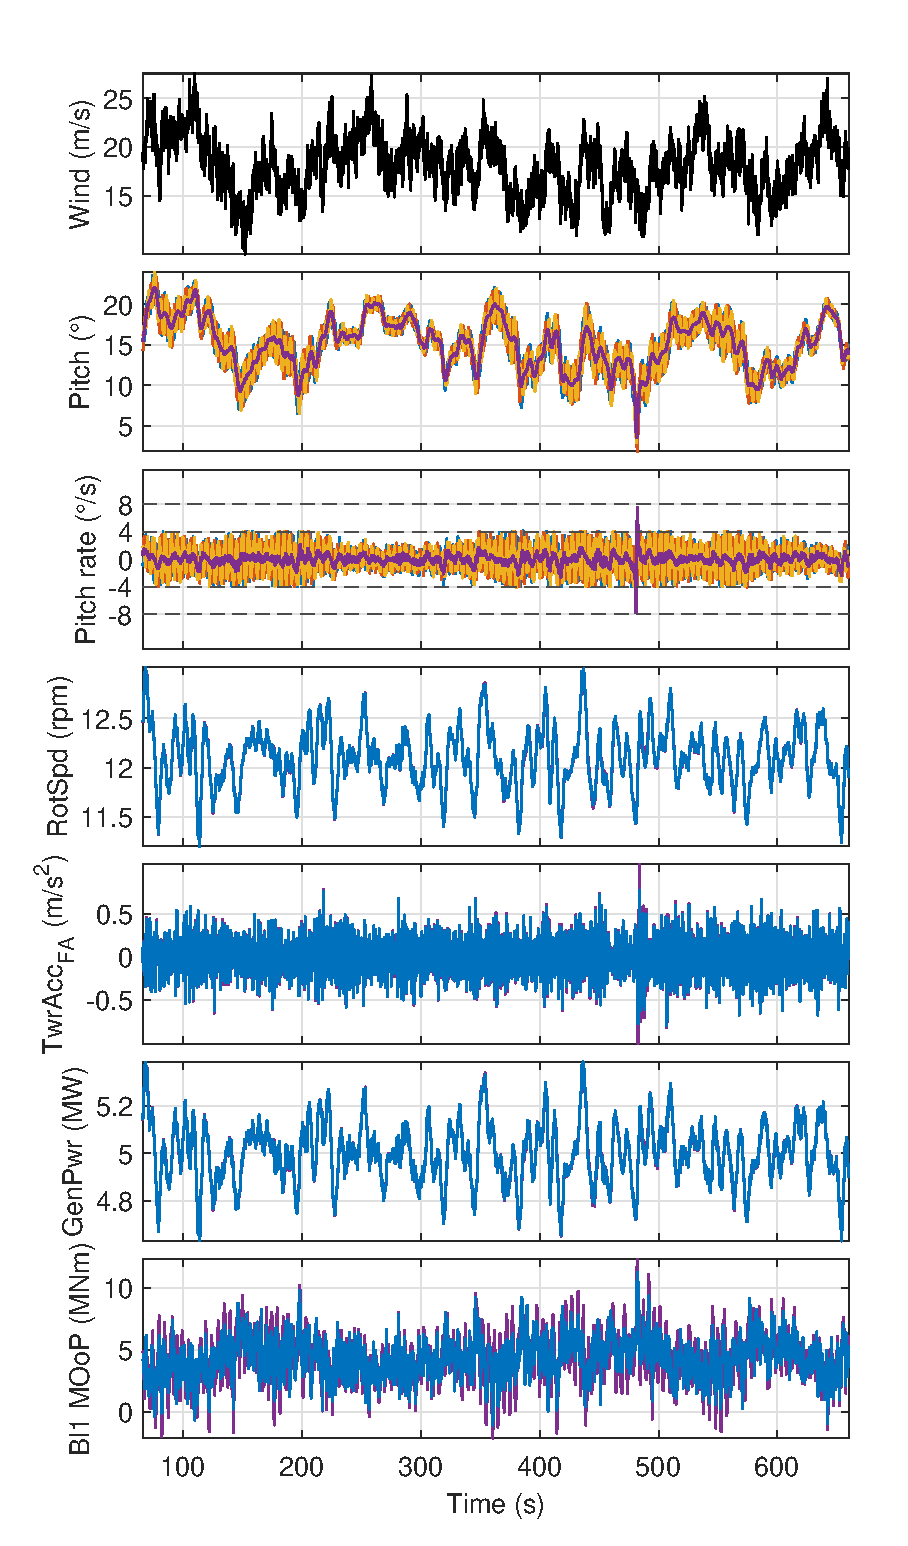
\includegraphics[width=0.495\textwidth,trim={0.cm 0cm 0cm 0.55cm}, clip]{figures/figIPCThesis/fig00a_Timeseries1.eps}}\hfill
    \subfloat[Pitch rate limit 13\textdegree/s, $K_{\text{P,IPC}}= 1.223$, $K_{\text{I,IPC}}= 0.365$]{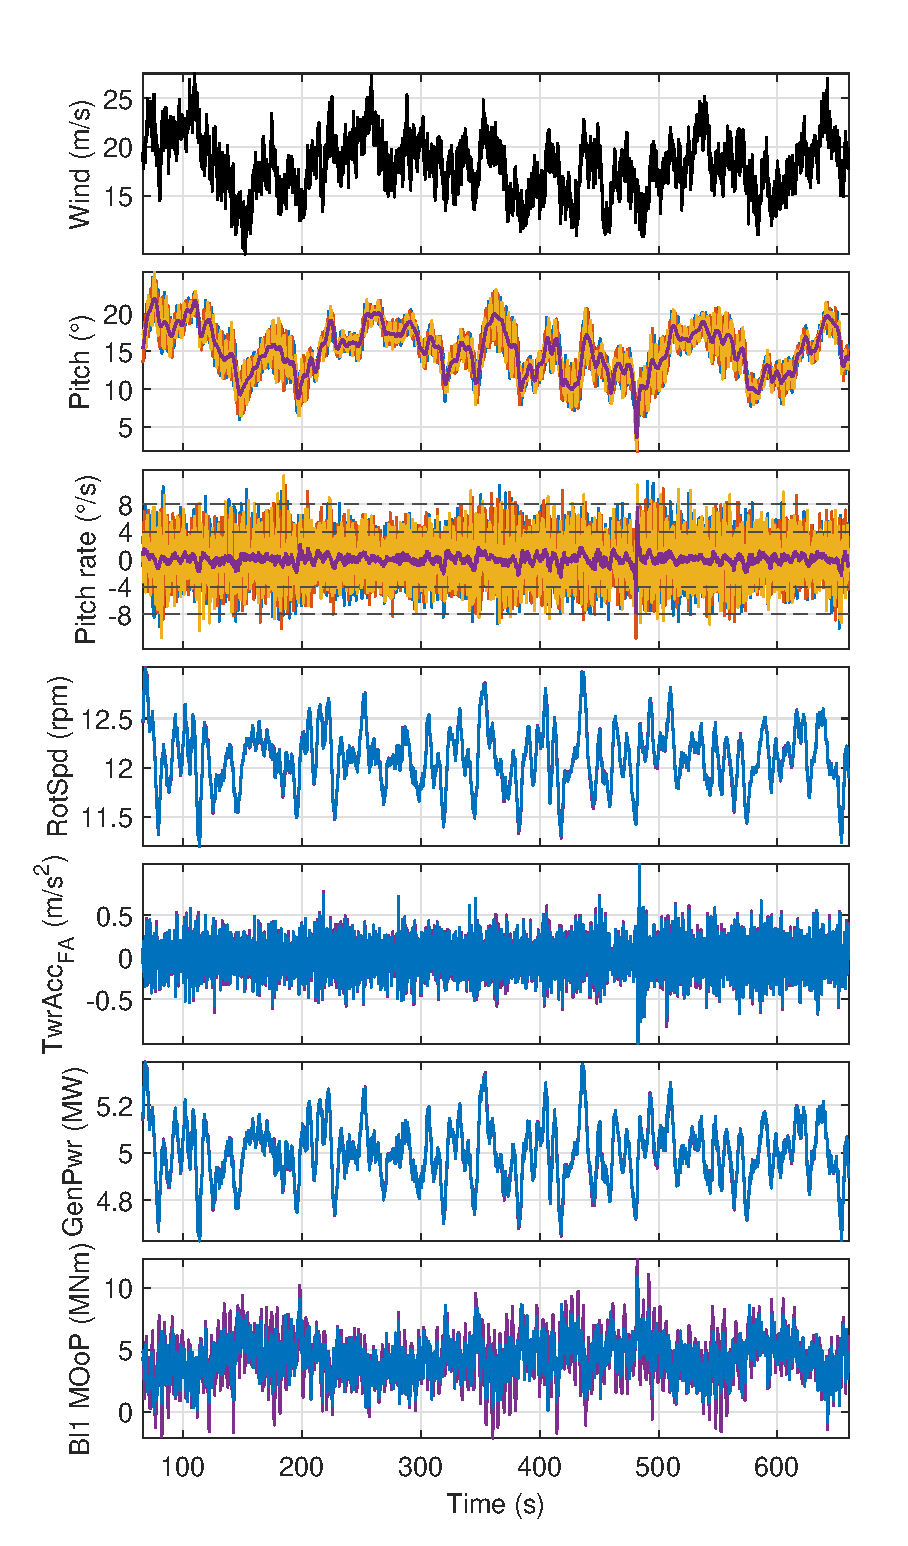
\includegraphics[width=0.495\textwidth,trim={0.cm 0cm 0cm 0.55cm}, clip]{figures/figIPCThesis/fig00a_Timeseries3.eps}}\hfill
    \caption[Controller comparison baseline CPC and IPC PI with different pitch rate limits.]{Controller comparison baseline CPC (\mlPurple) and IPC PI (\mlBlue, \mlOrange{} and \mlYellow{} pitch signals of blades 1 to 3, \mlBlue{} all other signals) with different pitch rate limits for turbulent wind (18\,m/s mean, turbulence class A, optimization dataset). Rate limits: Low (4\textdegree/s) and high (13\textdegree/s) for IPC, standard  (8\textdegree/s) for CPC PI. Dashed lines in the pitch rate plots: $\pm 4$\textdegree/s and $\pm 8$\textdegree/s. Displayed signals: freestream wind speed, pitch, pitch rate, states, power, and blade~1 root out-of-plane moment.}
    \label{fig:timeseriesIPC}
\end{figure}
%

%
Figure~\ref{fig:PSDIPC} shows the PSD of the blade root out-of-plane moment to visualize and explain the gradual improvement with increasing pitch rate for all three test cases. The black line represents the baseline CPC. The values given are the maxima of the PSD within 15\% of 1P and 2P. They represent the worst case in the vicinity of the rotor harmonics, which includes the spreading of the peaks due to the rotor speed variation and neighboring resonances. With IPC, the 1P peak is suppressed, so the value given is the largest PSD value in the 1P band rather than a distinct peak. The blue line, representing IPC with a 4\textdegree/s rate limit, reduces the 1P PSD peak by 91\%, while the orange line, representing IPC with an 8\textdegree/s rate limit, further lowers it, achieving a 96\% reduction. At the 2P frequency, the blue line shows only a small decrease of 11\% compared to the baseline, while the orange line lowers the 2P peak by 44\%. As expected, the 8\textdegree/s rate limit offers better load reduction across both 1P and 2P frequencies. The controller tuned with the rate limit set to 13\textdegree/s, depicted as a yellow dotted line, lies almost on top of the orange line, with 1P and 2P peak reductions of 96\% and 45\%, respectively.
\begin{figure}[h]
    \begin{center}
        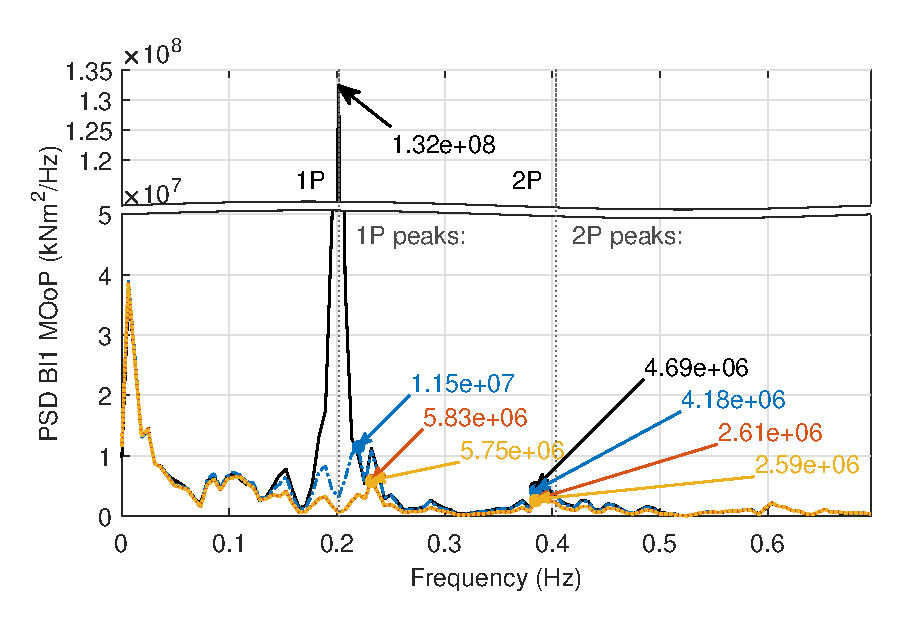
\includegraphics[width=0.6\textwidth]{figures/figIPCThesis/fig02_PSDroot_breaky_ratecomp.eps}
        \caption[Controller comparison: Power spectral density of the blade~1 root out-of-plane moment of baseline PI with 8\textdegree/s rate limit, IPC with 4\textdegree/s, 8\textdegree/s, and 13\textdegree/s rate limits]{Controller comparison: Power Spectral Density of the blade~1 root out-of-plane moment of baseline PI (\mBlack) with 8\textdegree/s rate limit, IPC with 4\textdegree/s rate limit (\mlBlueDashDot), 8\textdegree/s rate limit (\mlOrange), and 13\textdegree/s rate limit (\mlYellowDotted).}
        \label{fig:PSDIPC}
    \end{center}
\end{figure}
%
Table~\ref{tab:stddev_unified_IPC} summarizes the standard deviation of the signals shown in Figure~\ref{fig:timeseriesIPC} for IPC rate limits of 4\textdegree/s, 8\textdegree/s, and 13\textdegree/s. For all three cases, the baseline is the PI CPC with the standard rate limit of 8\textdegree/s. For the rotor speed and the power output, the introduction of IPC does not produce any observable effect, with ratios between 0.99 and 1.00. The tower fore-aft acceleration, whose differences are hardly visible in the time series, decreases slightly by 2\% to 3\%. The pitch rate standard deviation increases unavoidably for the IPC test cases: by a factor of 2.81 at the most restrictive limit of 4\textdegree/s, and by factors of 4.58 and 4.61 at 8\textdegree/s and 13\textdegree/s, respectively. In contrast, the blade root out-of-plane moment is reduced by 18\%, 25\%, and 25\% across the three limits, consistent with the spectral load reductions at 1P and 2P visible in Figure~\ref{fig:PSDIPC}.
\begin{table}[htbp]
    \centering
    \caption[Standard deviation of tower fore-aft acceleration, generated power, rotor speed, IPC blade pitch rate and blade root
    out-of-plane moment for turbulent wind.]{Standard deviation of tower fore-aft acceleration, generated power, rotor speed, IPC blade pitch rate and blade root
        out-of-plane (OoP) moment for turbulent wind (18\,m/s mean, turbulence class A) with different pitch rate limits, evaluated from 66\,s. Values in brackets show
        the ratio IPC/PI baseline (values below 1 indicate an improvement), with the PI baseline at the standard rate limit of 8\textdegree/s, whose standard deviations are 0.21\,m/s$^2$, 123.82\,kW, 0.30\,rpm, 0.65\textdegree/s, and 1986.63\,kNm, respectively.}
    \label{tab:stddev_unified_IPC}
    \begin{tabular}{l rrr}
        \toprule
        & \multicolumn{3}{c}{IPC rate limit (\textdegree/s)} \\
        \cmidrule(lr){2-4}
        Signal & low: 4 & standard: 8 & high: 13 \\
        \midrule
        Tower fore-aft acc.\ (m/s$^2$)  & 0.20 (0.98) & 0.20 (0.97) & 0.20 (0.98) \\
        Generated power (kW)             & 124.19 (1.00) & 123.30 (1.00) & 123.12 (0.99) \\
        Rotor speed (rpm)                & 0.30 (1.00) & 0.30 (1.00) & 0.30 (0.99) \\
        Blade pitch rate (\textdegree/s) & 1.83 (2.81) & 2.98 (4.58) & 3.00 (4.61) \\
        Blade 1 root OoP moment (kNm)    & 1624.02 (0.82) & 1483.35 (0.75) & 1481.16 (0.75) \\
        \bottomrule
    \end{tabular}
\end{table}
%
The IPC gains are optimized with a single wind field at 18\,m/s. To check whether they carry over to the whole of Region~III and to other wind fields, the IPC with the gains for 8\textdegree/s is simulated for all above rated wind speeds of the optimization dataset and of the two verification datasets, which are also used for the AALC in Section~\ref{subsec:ResultsTEF}. Table~\ref{tab:IPC_summary} contains the six evaluation criteria, normalized by simulations without IPC for the same wind test cases and averaged over three wind speed ranges: all wind speeds above rated, the wind speeds from 18\,m/s, and the optimization wind speed of 18\,m/s. As defined in Section~\ref{subsection: IPCOptCriteria}, the DELs are calculated with the W\"ohler exponents of 10 for the blades, summed over the three blades, and 4 for the tower, and all criteria are evaluated from 60\,s onward.
%
% Created by makeIPC_SummaryTable on 2026-10-26
\begin{table}[h]
    \centering
    \caption[Evaluation criteria for IPC: Mean values of the optimization and verification datasets over above-rated wind speed ranges]{\label{tab:IPC_summary} Evaluation criteria for IPC: Mean values of the optimization and verification datasets over above-rated wind speed ranges, normalized by the baseline PI without IPC; values below 1 indicate a reduction. IPC gains optimized at 18\,m/s with the pitch rate limit 8\textdegree/s: $K_{\text{P,IPC}} = 1.222$ and $K_{\text{I,IPC}} = 0.370$. Criteria are blade, tower
        base and tower top DELs, power mean and standard deviation, and pitch actuator power. The first verification set has no wind field for 13\,m/s.}
    
    %{ Evaluation criteria for IPC: Mean values of the optimization and verification datasets over the above rated wind speed ranges, normalized by the baseline without IPC. IPC gains optimized at 18\,m/s with the pitch rate limit 8\textdegree/s for all wind speeds: $K_{\text{P,IPC}} = 1.222$ and $K_{\text{I,IPC}} = 0.370$. Criteria are blade (sum of the three blades, W\"ohler exponent 10), tower base and tower top DELs (W\"ohler exponent 4, all evaluated from 60\,s), power mean and standard deviation (mean of the ratios of the single wind speeds), and actuator power (ratio of the mean actuator powers). The first verification set has no wind field for 13\,m/s.}
    \begin{tabular}{@{}l*{8}{c}@{}}
        \toprule
        Wind speeds & Dataset & Turb. class & $C_{\text{DEL},b}$ & $C_{\text{DEL},t,\text{Base}}$ & $C_{\text{DEL},t,\text{Top}}$ & $C_{\bar{P}}$ & $C_{\delta P}$ & $C_{\text{Act}}$ \\
        \midrule
        \multirow{3}{*}{\begin{tabular}[c]{@{}l@{}}Above rated\\(12--25\,m/s)\end{tabular}} & Optim. & A & 0.77 & 1.00 & 0.93 & 1.00 & 1.02 & 5.37 \\
        & Verif. 1 & A & 0.78 & 1.00 & 0.93 & 1.00 & 1.02 & 5.66 \\
        & Verif. 2 & B & 0.79 & 1.01 & 0.93 & 1.00 & 1.01 & 5.44 \\
        \midrule
        \multirow{3}{*}{18--25\,m/s} & Optim. & A & 0.75 & 1.01 & 0.94 & 1.00 & 1.01 & 5.84 \\
        & Verif. 1 & A & 0.76 & 1.01 & 0.95 & 1.00 & 1.01 & 5.97 \\
        & Verif. 2 & B & 0.75 & 1.02 & 0.93 & 1.00 & 1.01 & 5.89 \\
        \midrule
        \multirow{3}{*}{18\,m/s} & Optim. & A & 0.80 & 1.00 & 0.90 & 1.00 & 1.00 & 5.04 \\
        & Verif. 1 & A & 0.79 & 1.00 & 0.92 & 1.00 & 1.00 & 5.01 \\
        & Verif. 2 & B & 0.80 & 1.06 & 0.91 & 1.00 & 1.00 & 5.01 \\
        \bottomrule
    \end{tabular}
\end{table}


Above rated, the blade DEL decreases by 21\% to 23\%, and from 18\,m/s on by 24\% to 25\%, for all three datasets. The reduction grows with the wind speed: for the second verification set of turbulence class~B, it increases from 11\% to 16\% between 12 and 16\,m/s to 25\% to 27\% from 20\,m/s on. The gains optimized at a single wind speed hence carry over to the whole of Region~III and to both verification sets, so that no gain scheduling is required above rated. The tower base DEL is not changed considerably, with criteria between 1.00 and 1.01; the largest increase of a single wind speed is 6\% at 18\,m/s for turbulence class~B. The tower top DEL is reduced by about 7\% above rated and by 8\% to 10\% at 18\,m/s. Close to rated wind speed, the mean power decreases by up to 0.6\% and its standard deviation increases slightly, so that the power criteria above rated are 1.00 and 1.01 to 1.02. The pitch rate reaches the limit of 8\textdegree/s at all wind speeds, and the actuator power is increased by a factor of 5.4 to 5.7 above rated and of 5.8 to 6.0 from 18\,m/s on. Compared with the AALC (Table~\ref{tabone}), the IPC achieves about the same blade DEL reduction above rated (AALC: 22\% to 24\%), but at a clearly higher actuator power (AALC: factor 3.9 to 4.0); from 18\,m/s on, the AALC reduces the blade DEL slightly more (26\% to 27\%).


IPC was shown in this section to reduce blade loads, with the amount of reduction progressively increasing with higher pitch rate limits, at the cost of increased actuator energy. It was also shown to decrease tower loads to a certain degree. The IPC gains optimized at a single wind speed of 18\,m/s carry over to the whole of Region~III and to both verification datasets, with blade DEL reductions of 21\% to 23\% above rated at unchanged tower base DEL and power, but with an actuator power increased by a factor of 5.4 to 5.7. 
On the qLPV model without model mismatch, the qLMPC discussed in the previous section reduces the tower loads more effectively than IPC, as it directly controls the collective pitch to lower thrust fluctuations. On FAST, however, the adapted qLMPC designs increase the tower loads and do not reduce the blade loads, while IPC reduces the blade DEL without wind information. The performance of IPC also depends on the quality of the blade root out-of-plane moment measurements. Nevertheless, IPC PI controllers are currently more widely accepted as a relatively simple method for reducing blade loads on large turbines. A combination of qLMPC and IPC is investigated in Section~\ref{subsec:ComparisonWindTurbineControlDesigns}.

While this section focused on load mitigation through individual pitch control, further 
improvements can be achieved by including additional actuators. As blade sizes continue to 
increase, additional actuation devices integrated into the blade structure might become 
necessary. The following section introduces a turbine model enhanced 
with trailing edge flaps on the rotor blades, enabling combined IPC and flap control for 
more effective high-frequency load reduction.

\let\oldsectionmark\sectionmark
\renewcommand{\sectionmark}[1]{\oldsectionmark{Combined IPC-TEFC Design and Application}}
\section{Combined IPC and Trailing Edge Flap Control Design and Application}
\label{sec:CombinedIPC-TrailingEdgeFlapControl}
\let\sectionmark\oldsectionmark

Building on the previous investigations into IPC and qLMPC strategies, this section focuses on a combined control approach that incorporates both IPC and TEFs. By including TEFs in the rotor blades as supplementary actuation surfaces, additional degrees of freedom become available for targeted load mitigation, particularly at higher frequencies. This combination of individual pitch and trailing edge flap control is referred to as IPC-TEFC or AALC. AALC is defined as the integrated use of multiple aerodynamic actuators to actively reduce structural loads while preserving power output. By coordinating both individual blade pitch adjustments and trailing edge flap deflections, AALC can provide enhanced load mitigation compared to each method alone. This section presents the model formulation for incorporating TEFs into the wind turbine dynamics and evaluates a combined IPC-TEFC strategy across Regions~II and~III. The controller design is based on an optimization framework that considers multiple wind conditions and turbulence intensities to ensure good performance over the whole operating range. Several DLR studies have addressed TEFC optimization. In \cite{kumar2019load}, a first proof of concept is implemented. The TEFC scheme from that work is fine-tuned in \cite{adolph2022reglerparameteroptimierung}. In \cite{osterwinter2023load}, the parameters of a combined IPC-TEFC approach are optimized and validated using a comprehensive set of verification wind fields to assess load reduction, power preservation, and actuator demand. Results from this report are published in \cite{dittmer2024combined}.


\subsection{TEF Simulation Model} %bonnie_jonkman_openfastopenfast_2022 OpenFAST2023
As before, the OpenFAST simulation software is used to investigate the benefits of combining individual pitch and trailing edge flap control. The NREL 5MW wind turbine model is modified to implement controllable trailing edge flaps on the rotor blades. The original NREL 5MW model without TEF serves as a reference for analyzing the aerodynamic effects of these modifications on the simulated operation of the turbine. 
\subsubsection*{Rotor Blade Geometry and Aerodynamics}
The rotor blades of the NREL 5MW turbine are defined by eight distinct cross-sectional profiles distributed along the blade length, as illustrated in Figure~\ref{subfig:TEF1}, and comprise 19 nodes, each with specific geometric profile shapes. At the root, cylindrical profiles connect to the rotor hub, accommodating high bending moments and pitch adjustments. The profiles transition from the DU series, developed at Delft University of Technology, near the root to the NACA64 profile in the outer 29\% of the blade, characterized by decreasing thickness towards the tip. The blade's aerodynamic efficiency is further refined by varying the profile depth and orientation at each node.

The blade section with trailing edge flaps, which covers the whole NACA64 blade section, is marked in red. The flap-to-blade chord ratio amounts to 20\%. The aerodynamic model of the blade enhanced with TEF requires input data on lift, drag, and pitching moment coefficients for all profiles across various blade angles of attack and a variety of flap deflection angles. The three main factors influencing these aerodynamic properties are surface roughness, Mach number, and Reynolds number. The OpenFAST simulation neglects surface roughness variations due to contaminants. The airflow is assumed to be incompressible with a Mach number of 0.25 at the blade tip. OpenFAST can interpolate between polars based on either the Reynolds number or a user-defined parameter. In this work, the user-defined parameter is the flap angle, i.e., the interpolation is performed between the polars of the different flap angles. As only one interpolation parameter can be defined, the Reynolds number distribution depicted in Figure~\ref{subfig:TEF1} is used for all wind speeds. Reynolds numbers ranging from one to eight million are obtained from an OpenFAST simulation with turbulence class A at a mean wind speed of 12\,m/s. Care was taken to model the distribution of Reynolds numbers along the rotor blade at this wind speed as realistically as possible. The OpenFAST aerodynamic models of the rotor blades are extended with additional airfoil polars based on this distribution.  % with the numbers obtained via an OpenFAST simulation run with a wind file from the optimization dataset, with turbulence class A and the meand wind speed at 12\,m/s.
\begin{figure}[h]
    \centering
    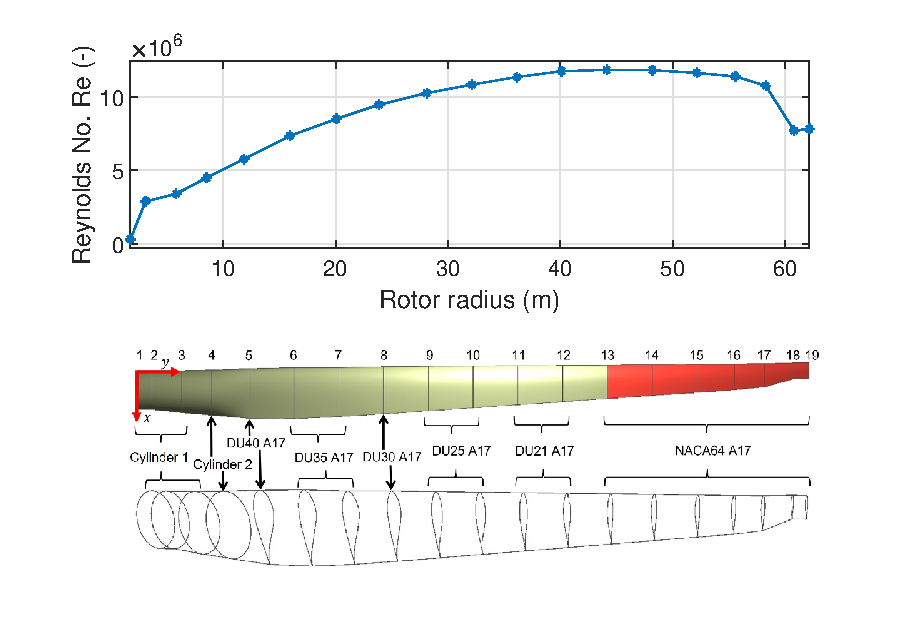
\includegraphics[width=0.6\textwidth]{figures/Images_Torque24/fig01_RE.eps}\hspace{0pc}%
    \begin{minipage}[b]{0.95\textwidth}\caption[ Span-wise distribution of Reynolds numbers Re at wind speed $V_{\infty} = 12$\,m/s]{\label{subfig:TEF1} Span-wise distribution of Reynolds numbers Re at wind speed $V_{\infty} = 12$\,m/s (from OpenFAST simulation) and blade geometry with cylinder, DU40, DU35, DU30, DU25, DU21 and NACA64 profiles with TEF location covering the NACA64 section marked in red.}
    \end{minipage}
\end{figure}

\subsubsection{Polar Calculation with xflr5 and XFOIL}
The aerodynamic coefficients of rotor blade profiles for the TEF-enhanced blades are calculated using the programs xflr5 and XFOIL, see \cite{drela1989xfoil}. XFOIL uses a higher-order panel method to analyze and design airfoil profiles, incorporating variables like Reynolds number, Mach number, and a transition criterion for calculating the shift from laminar to turbulent flow. The turbulence degree of the incoming flow determines the appropriate transition criterion value, with the default value set at 9, approximating a median turbulence level as per XFOIL's documentation. For fluid properties, standard sea-level values from the International Standard Atmosphere (ISA) are used. The aerodynamic coefficients for the respective profiles are calculated based on the Reynolds numbers selected from Figure \ref{subfig:TEF1}. The coefficients generated by xflr5 and XFOIL are not directly suitable for wind turbine simulation as AeroDyn15 requires coefficients over an angle of attack range from -180\textdegree{} to +180\textdegree. Since XFOIL's panel methods yield accurate results only up to the point of flow separation, the polars are extrapolated to cover the entire required angle range. This extrapolation is performed using the AirfoilPrep preprocessor developed by NREL, applying the Viterna method for extrapolating polars, see for details e.g.~\cite{gasch2011wind}. %on Viterna's calculation process 
Additionally, corrections are made to account for three-dimensional flow effects caused by the rotor blade's rotation. Factors like Coriolis and centrifugal forces increase the maximum lift coefficients in the inner rotor areas. These 3D effects are corrected using functions integrated into AirfoilPrep. Figure \ref{subfig:TEF2} illustrates the extrapolated and corrected lift and drag coefficients over the angle of attack for rotor blade profiles with different flap angles. 

Figure~\ref{subfig:TEF2}\,(a) shows that a positive flap deflection increases the lift coefficient $c_l$ and hence the lift. A positive flap deflection $\eta_{\text{TEF}}$ is defined as the trailing edge of the flap moving towards the pressure side, relative to the chord line of the local blade profile with undeflected flap. The maximum lift coefficient occurs at a smaller angle of attack than with a neutral flap position. A negative flap deflection has the opposite effect: the lift coefficients are reduced and the maximum lift coefficient shifts to higher angles of attack. This corresponds to the expected effect of trailing edge flap deflections on the lift. 
%
\begin{figure} [htbp]
    \centering
    \subfloat[Lift coefficient $c_{l}$]{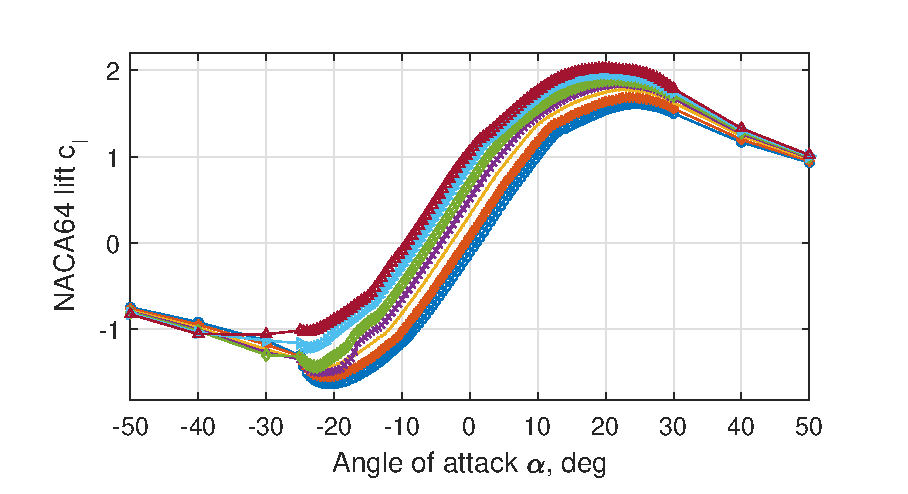
\includegraphics[width=0.495\textwidth,trim={0.cm 0cm 0cm 0.5cm}, clip]{figures/Images_Torque24/fig01_Cl1out.eps}}\hfill 
    \subfloat[Drag coefficient $c_{d}$]{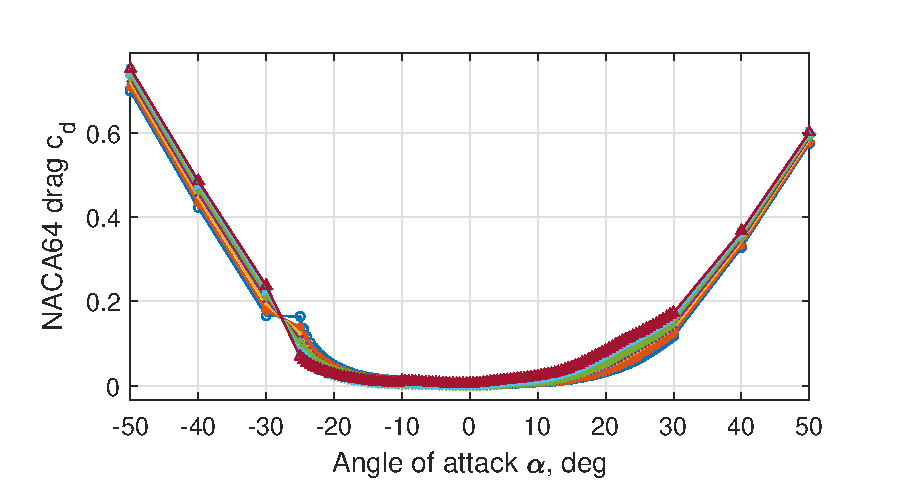
\includegraphics[width=0.495\textwidth,trim={0.cm 0cm 0cm 0.5cm}, clip]{figures/Images_Torque24/fig01_Cd1out.eps}}   
    \caption[Lift and drag coefficients at different trailing edge flap angles $\eta_{\text{TEF}}$ and blade angles of attack $\alpha$]{Lift and drag coefficients over the blade angle of attack $\alpha$ for the trailing edge flap angles $\eta_{\text{TEF}} = -10^\circ$ (\mlBlueCircle), $-7^\circ$ (\mlOrangeStar), $-3^\circ$ (\mlYellowLine), $0^\circ$ (\mlPurpleCross), $3^\circ$ (\mlGreenDiamond), $7^\circ$ (\mlCyanTriangle), and $10^\circ$ (\mlMaroonTriangle). The data are physically plausible for $-27^\circ \le \alpha \le 30^\circ$.}
    \label{subfig:TEF2}
\end{figure}
Figure~\ref{subfig:TEF2}\,(b) shows the drag coefficient. The curves of the drag coefficient $c_d$ are smooth and physically plausible for angles of attack above $-27^\circ$. Below this value, the vertical order of the polars suddenly reverses. There is no physical explanation for this effect, and no such discontinuity occurs for the rotor profile without trailing edge flap. Presumably, the extrapolation method does not work well for flapped profiles at these large negative angles of attack, where flow separation and stall occur. However, this can be disregarded, as the angles of attack in the outer region of the rotor blades do not fall below $-27^\circ$ during normal operation. As this study uses OpenFAST v3.2.1, no additional code is needed to include the TEF, unlike earlier studies based on previous FAST versions. The obtained coefficients are stored in an airfoil file, which is referenced in the Airfoil Information section of the AeroDyn15.dat file of the NREL 5MW model available in the Git repository~\cite{GitRepoCodeAALC}. %NACA64_A17_Flap.dat

%
\subsubsection*{Baseline Power Controller} %speed-controlled-pitch-controlled
In order to realistically simulate a modern turbine, a control system controlling rotor speed and generator torque is required, and the same baseline controller described and applied in the previous sections is utilized for that purpose. The aim of the IPC-TEFC is to further decrease the mechanical loads. Note that this load reduction controller using IPC together with TEF control is an add-on controller to the baseline control system. This is possible as cyclic pitch motions are induced, which are effectively decoupled from the collective pitch motion, ensuring rated power output above rated wind speed. As before, the implementation of the baseline controller is the power controller available within TU Delft's FASTTool, see \cite{mulders2020wind}. 
%
\subsubsection*{Open-Loop TEF Model Verification with FAST} % with TEF open loop control
The modified NREL 5MW turbine model presented in the previous section is tested in open-loop simulations with regard to the plausibility of the influence of the TEF position on the simulation results. The aerodynamic model of the trailing edge flap is included. Open-loop control inputs of the TEF deflection angle $\eta_{\text{ref}}$ are analyzed in order to investigate its suitability with regard to the desired DEL reduction. The effects of flap deflections on different parameters relevant to the operational quality of the wind turbine, such as forces and moments as well as power yield, are investigated. Figure \ref{fig:OLdiag} shows a block diagram to illustrate the control structure used for these verification tests, with the eight inputs, i.e., the seven control inputs and the wind of the selected test case $V_{\text{TC}}$ as a disturbance. The actuators for the pitch angle adjustment of the rotor blades are modeled as a first-order transfer function with position and rate limitations. The influences of different TEF positions for steady-state operating conditions are discussed in Section~\ref{subsec:ResultsTEF}. 
% For a sensitivity study of the flaps with regard to their influence on the blade root flapping moments, we refer to \cite{osterwinter2019load1}.
\begin{figure}[h]
    \centering
    \includegraphics[width=0.95\textwidth, trim=0 0 0 13, clip]{figures/Images_Torque24/blockdiagram_OL_latex_tau2.pdf}\hspace{2pc}%
    \begin{minipage}[b]{0.95\textwidth}
        \caption[Block diagram for open-loop TEF verification tests.]{\label{fig:OLdiag} Block diagram for open-loop TEF verification tests: the power control, consisting of the gain-scheduled PI pitch control and the $k\omega_g^2$ torque control, operates in closed loop on the generator speed $\omega_g$, while all three flaps receive the same constant reference $\eta_{\text{ref}}$ in open loop. The wind $V_{\text{TC}}$ of the respective test case acts as a disturbance.}    
        
        
        %\caption{\label{fig:OLdiag} Block diagram for open-loop TEF verification tests with baseline power control in closed loop and open-loop collective TEF control inputs.}
    \end{minipage} %BlockschaltbildopenLoop1.jpg
\end{figure}

%\caption[Block diagram for open-loop TEF verification tests]{\label{fig:OLdiag} Block diagram for open-loop TEF verification tests: the baseline power control, consisting of the gain-scheduled PI pitch control and the $k\omega_g^2$ torque control, operates in closed loop on the generator speed $\omega_g$, while all three flaps receive the same constant reference $\eta_{\text{ref}}$ in open loop. The wind $V_{\text{TC}}$ of the respective test case acts as a disturbance.}

\subsection{IPC-TEFC Implementation}
The main design objective of the presented AALC is the reduction of structural moments, focusing on the out-of-plane blade root bending moments. The overall controller layout is shown in Figure~\ref{fig:CLdiag}. The baseline controller, depicted in Figure~\ref{fig:OLdiag}, is enhanced with IPC, with the individual pitch demand added to the collective pitch reference, as well as TEFC which changes the TEF position. All six AALC control output signals are calculated via MBC, see Section \ref{sec:MBC}, based on the three out-of-plane blade root moments, $M_{yc1}$, $M_{yc2}$, and $M_{yc3}$, as well as the rotor azimuth $\theta_r$. This section reviews the allocation of IPC and TEFC signals and then discusses the design of these controllers. 
\begin{figure}[h]
    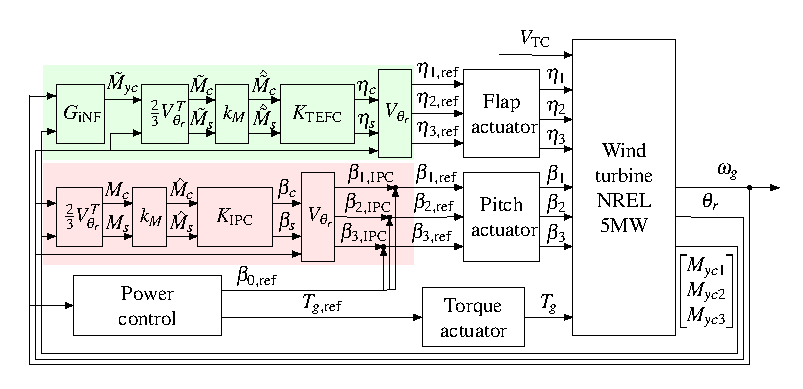
\includegraphics[width=0.95\textwidth]{figures/Images_Torque24/blockdiagram_CL_latex2.pdf}\hspace{2pc}%
    \begin{minipage}[b]{0.95\textwidth}  
        \caption[Block diagram of the closed-loop AALC with baseline power control, IPC, and TEFC]{\label{fig:CLdiag} Block diagram of the closed-loop AALC: the power control sets the collective pitch and generator torque references. The IPC (red) transforms the blade root moments $M_{yci}$ via MBC into the tilt and yaw moments, whose controller outputs are transformed back into individual pitch demands added to $\beta_{0,\text{ref}}$. The TEFC (green) has the same structure, but the inverse notch filter $G_{\text{iNF}}$ emphasizes the 2P loads, and the outputs are the flap references $\eta_{i,\text{ref}}$.}
        
    \end{minipage}
\end{figure}

%

%       \caption[Block diagram for closed-loop TEF verification tests with baseline power control, individual pitch and TEF closed loop control.]{\label{fig:CLdiag} Block diagram for closed-loop verification tests with baseline power control, individual pitch (highlighted in red) and TEF (highlighted in green) closed loop control.}

\subsubsection*{IPC and TEFC Control Allocation}
As for the IPC, the rotating blade root out-of-plane moments are transformed into the fixed coordinate system via MBC, see Section~\ref{sec:MBC} and Equation~\eqref{eq:MBC}.

Figure~\ref{fig:CLdiag} denotes $M_{yci}$ as the out-of-plane blade root moment of the $i$-th blade as inputs, and the rotor tilt moment $M_c$ and yaw moment $M_s$ in the non-rotating system as outputs. The moments $M_c$ and $M_s$ are used to calculate two cyclic control signals $q_c$ and $q_s$, i.e., $\beta_c$ and $\beta_s$ for IPC, and $\eta_c$ and $\eta_s$ for TEFC. The control signal $q_i$ of the $i$-th blade is calculated via the inverse MBC transformation in Equation~\eqref{eq:inverseMBC},
where the signal $q_i$ denotes $\beta_{i,\text{IPC}}$ and $\eta_{i,\text{ref}}$ in IPC and TEFC, for the $i$-th blade or flap, respectively. As for the IPC scheme, the tilt and yaw moments $M_c$ and $M_s$ are controlled via $q_c$ and $q_s$ independently, i.e., any remaining coupling following the MBC transformation between $q_c$ and $M_s$ as well as $q_s$ and $M_c$ is neglected. As the wind turbine dynamics can be approximated as an LTI system after transforming rotor blade dynamics into a fixed coordinate system, using MBC from Equation~\eqref{eq:MBC}, a simple, intuitive control approach is adopted. Four separate SISO controllers, two each for IPC and TEFC, are designed to reduce the transformed moments $M_c$ and $M_s$. The system is now over-actuated, i.e., two moments, $M_c$ and $M_s$, need to be mitigated, but four control inputs, $\eta_c$, $\eta_s$, $\beta_c$, and $\beta_s$, are available. This offers the possibility of a frequency separation as a form of control allocation. To achieve this frequency separation of IPC and TEFC, inverse notch filters are implemented in the AALC controller. The 1P loads in the frequency spectrum of the blade root bending moments are addressed with the IPC control loop. The 2P loads are addressed with the trailing edge flap controller making use of the fast flap dynamics. While modern MIMO controllers, e.g., AALC extension of the $H_\infty$ control \cite{ossmann2021field,ossmann2017load} or MPC \cite{dittmer2021velocity}, have the potential to optimize the available control inputs regarding the criteria listed in Section~\ref{sec:ControllerParameterOptimization} more efficiently, this simple, intuitive control allocation is selected as the resulting controller does not employ an observer-based structure and hence does not require the design of an explicit mathematical plant model.%via strategies such as MPC, LQG or $H_\infty$ control. %Details are elaborated below.

\subsubsection*{Individual Pitch Control for 1P Load Reduction}
The IPC controller $K_{\text{IPC}}$, illustrated in the red part of Figure \ref{fig:CLdiag}, receives the blade root out-of-plane moments $M_{yc1}$, $M_{yc2}$, and $M_{yc3}$ from the rotating coordinate systems, transforming them into fixed coordinate system moments $M_c$ and $M_s$ via MBC without additional filtering. This approach obviates the need for low-pass filtering within the IPC loops, as the actuator models already provide inherent low-pass filtering characteristics. The transformed moments are scaled with $k_M = 10^{-5}$, a value chosen due to the order-of-magnitude difference between the moments and the control angles in units of radians. The scaled moments $\hat{M}_s$ and $\hat{M}_c$ are passed to two identical SISO controllers. These controllers are based on the assumption that the transformed moments become largely independent after the transformation. The LTI nature of the transformed system allows for the potential use of PI controllers. Moreover, for IPC, which focuses on mitigating low-frequency load changes, particularly the 1P loads caused mainly by wind shear, a controller with an integral gain is first tuned manually. The integral component adequately addresses the control requirements by minimizing the steady-state error of the transformed moments and thus effectively targets the minimization of the 1P loads in the rotating coordinate system. This aids in decoupling the IPC from the TEFC controller, with the TEFC used for controlling higher frequencies. The calculated control signals $\beta_c$ and $\beta_s$ are converted back to the rotating blade coordinate systems via the inverse MBC given in Equation~\eqref{eq:inverseMBC}, resulting in the three signals $\beta_{i,\text{IPC}}$. The IPC exclusively calculates individual pitch angle components, avoiding interference with collective pitch angles calculated by the baseline power controller. The pitch angle commands, passed to the pitch actuators, $\beta_{i,\text{ref}}$ are calculated by adding the collective pitch angle command $\beta_{0,\text{ref}}$ to these individual pitch reference signals. The actuator model is implemented as a first-order transfer function with time constant $\tau_{\beta}=0.1$\,s with the angle limited from -2\textdegree{} to 90\textdegree{} and the rate limited from -8\textdegree{}/s to 8\textdegree{}/s. The pitch actuator angles $\beta_i$ are then applied to the OpenFAST NREL 5MW wind turbine model.

\subsubsection*{Trailing Edge Flap Control and Inverse Notch Filter for 2P Load Reduction}
The controller for the individual trailing edge flap control $K_{\text{TEFC}}$ is constructed similarly to the IPC: the MBC and inverse MBC enclose two identical SISO controllers for the transformed moments.

A key difference is that the blade root out-of-plane moment signals are filtered through an inverse notch filter before MBC processing, amplifying selected frequencies
\begin{equation*}
    G_{\text{iNF}}(s) = (s^2 +2k_{\text{iNF}}D\omega_{\text{iNF}}s +\omega_{\text{iNF}}^2)/ (s^2 +2D\omega_{\text{iNF}}s +\omega_{\text{iNF}}^2),\quad k_{\text{iNF}}=10,\quad D = 0.1
\end{equation*}
with the frequency $\omega_{\text{iNF}} = 2 \cdot 2\pi f_r$, i.e., twice the current rotor frequency $f_r$, and $s$ being the Laplace variable. This enhances 2P load amplitudes in the signals, enabling the TEFC to predominantly respond to these loads, thus minimizing mutual influence with the IPC. Post-filtering, the three blade root out-of-plane moments $\tilde{M}_{yci}$ are transformed into the fixed coordinate system via a multiplication with $2/3 V^T_{\theta_r}$, with the resulting moments $\tilde{M}_{c}$ and $\tilde{M}_{s}$. These are both scaled with $k_M$ to $\hat{\tilde{M}}_c$ and $\hat{\tilde{M}}_s$. Initially, two proportional controllers are used, with the manually tuned proportional parameter used as a starting point for the optimization of the controller parameters. The transformed control outputs are then converted back for flap angle adjustments, with flap actuators modeled for a more rapid response than the pitch actuators, aiding in 2P load reduction. The TEF actuator is modeled as a first-order transfer function with time constant $\tau_{\eta}=0.05$\,s, with the angle limited from -10\textdegree{} to 10\textdegree{}, and the rate limited from -20\textdegree{}/s to 20\textdegree{}/s.

\subsection{IPC-TEFC Parameter Optimization} \label{sec:ControllerParameterOptimization}
As for IPC, the AALC gains at 18\,m/s are optimized with \textit{fminsearch} followed by \textit{fmincon} with the tower constraint, for the pitch rate limit of 8\textdegree/s and with the fade-in of the IPC and TEF inputs. The procedure is as follows:
\begin{enumerate}
    \item A preliminary optimization of the proportional TEFC gain $K_{\text{P,TEFC}}$ is run with fixed IPC gains ($K_{\text{P,IPC}} = 0.62$, $K_{\text{I,IPC}} = 0.32$, from an IPC optimization before the fade-in was introduced). The integral and derivative gains of the TEFC, $K_{\text{I,TEFC}}$ and $K_{\text{D,TEFC}}$, are set to zero; a joint optimization of $K_{\text{D,TEFC}}$ resulted in a value close to zero ($K_{\text{D,TEFC}} = 0.002$) without a noticeable decrease of the cost. A TEF integral gain would shift the low-frequency control effort at 1P from the pitch to the flaps. It would lower the pitch activity but raise the flap activity, for a negligible blade DEL gain. It was therefore not used. For this optimization step, only \textit{fminsearch} is used to optimize the proportional gain, resulting in $K_{\text{P,TEFC}} = 0.24$.
    \item The proportional and integral gains of the IPC and the proportional gain of the TEFC are optimized jointly at 18\,m/s, starting from the IPC gains optimized for 8\textdegree/s ($K_{\text{P,IPC}} = 1.22$, $K_{\text{I,IPC}} = 0.37$) and $K_{\text{P,TEFC}} = 0.24$ from the preliminary optimization. In this step, \textit{fminsearch} is followed by \textit{fmincon}. As the result of \textit{fminsearch} already satisfies the tower constraint, \textit{fmincon} does not change it.
\end{enumerate}
Below rated, the three gains are optimized jointly for each of the wind speeds 4, 6 and 8\,m/s, with \textit{fminsearch} only, since the tower DEL decreases below rated anyway and the tower constraint is not needed. The optimization is started from the initial gains of \cite{dittmer2024combined}, i.e., a purely integral IPC and a purely proportional TEFC, each with a gain of one.


As for the IPC, the quality of an AALC controller is quantified via the decrease in blade root DEL. The cost function $J$ to be minimized by the AALC is the maximum of the DEL of the three blades, i.e., the same cost function as provided in Equation~\eqref{eq:costFunIPC}.
To evaluate and quantify the impact of an AALC controller's performance, the same criteria as before are used, which can be summarized as follows:

\begin{itemize}
    \item \textbf{Blade DEL $C_{\text{DEL},b}$ and tower DEL $C_{\text{DEL,t}}$:} Reducing the blade DEL is the main incentive for using
    IPC to decrease the PSD at 1P. Load reductions at the 1P frequency do
    not directly influence the tower base DEL, while decreasing the PSD at the 2P frequency via the
    flaps also decreases the tower top DEL. Therefore, a decrease in tower top DEL is observed although this criterion is not included in the objective function.  
    \item \textbf{Power mean $C_{\bar{P}}$ and standard deviation $C_{\delta P}$:} The power criteria were also not included in the
    optimization. As the annual energy production is typically not allowed to decrease from AALC,
    the generated power was compared for all test cases above rated and it was found
    that the power production loss and variance increase are negligible. % The power
    %variance is important for the stability in small networks. The effect of the AALC controller was found to be nearly negligible.
    \item \textbf{Actuator power $C_{\text{Act}}$:} This is the only criterion for which an increase is
    unavoidable, due to the additional movement of the blade that
    the IPC requires; the flap actuators are not included in this criterion. %With the activation of individual pitch control, the pitch actuator power tripled to approximately 4.5 kW for all pitch actuators.
\end{itemize}
As for the IPC, the optimization dataset with wind of turbulence class~A is used to optimize the parameters at 18\,m/s above rated and, in addition, at 4, 6, and 8\,m/s below rated. As before, the pitch rate limit is fixed at 8\textdegree/s. The AALC's effect is analyzed by incorporating five wind speeds in Region~II, from 4\,m/s to 11\,m/s, and nine wind speeds in Region~III, ranging from 12\,m/s to 25\,m/s. Two verification sets are created for the 14 wind speeds, with the wind fields for 11 and 13\,m/s missing in the first one: one with turbulence class~A using a different seed, and one with turbulence class~B. The vertical wind speed distribution is modeled with a power law wind profile to represent wind shear, using an exponent of 0.2. All wind fields are available in the Git repository \cite{GitRepoCodeAALC}, which also includes the code to reproduce all results presented here. 

\subsection{Results} \label{subsec:ResultsTEF}
This section discusses both open-loop results, obtained with the simulation setup depicted in Figure~\ref{fig:OLdiag}, and closed-loop results, simulated with the control loop from Figure~\ref{fig:CLdiag}. 

\subsubsection{Open-Loop Results}
Figure~\ref{fig:OLval} shows the steady-state values, at three different TEF angles, of power $P_g$, rotor speed $\omega_r$, rotor thrust $F_{T_r}$, and blade pitch angle $\beta_{0}$ for all 14 wind speeds. Simulations at constant wind speeds are run for 660\,s to confirm the plausibility of the TEF model. Data from the initial 60\,s are excluded to avoid non-physical initialization artifacts and the mean values are calculated for each wind speed.
\begin{figure} [htbp]\centering
    \centering
    % \subfloat[Power and rotor speed]{\includegraphics[width=0.65\textwidth]{figures/Images_Torque24/fig06_TEFOL_1.eps}}\\
    % \subfloat[Rotor thrust and blade pitch]{\includegraphics[width=0.65\textwidth]{figures/Images_Torque24/fig06_TEFOL_2.eps}}
    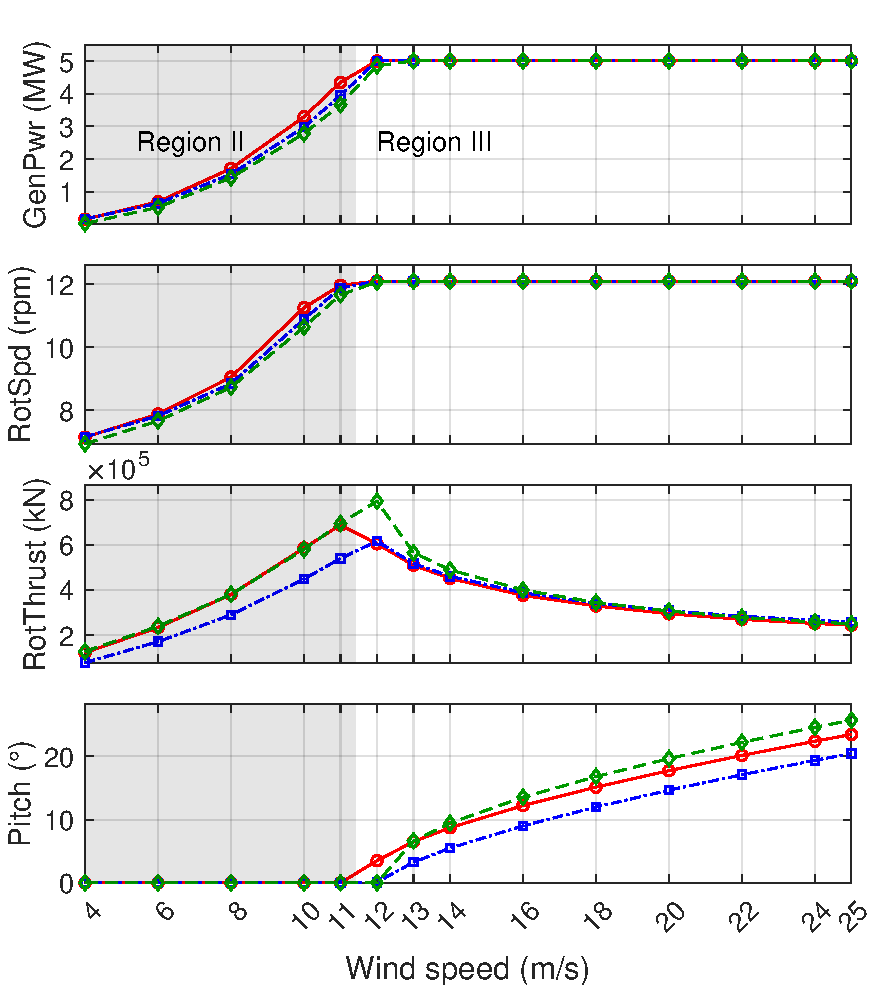
\includegraphics[width=0.6\textwidth]{figures/Images_Torque24/fig06_TEFOL.pdf}
    \caption[TEF open-loop verification: Mean values for TEF deflections of -10\textdegree{}, 0\textdegree{}, and 10\textdegree{} for constant wind.]{TEF open-loop verification: Mean values for TEF deflections of -10\textdegree{}\,(\mlBlueDashDotSquare), 0\textdegree{}\,(\mlRedCircle), and 10\textdegree{}\,(\mlDarkGreenDashedDiamond) for constant wind. Region~II and Region~III marked with gray and white backgrounds, respectively. Displayed signals: Power, rotor speed, rotor thrust, and blade pitch.}
    \label{fig:OLval}
\end{figure}

%
The simulated power with and without TEF deflections shows the expected power characteristic curve of a wind turbine: In Region~II, both positive and negative flap deflections reduce power \(P_g\) due to decreased aerodynamic efficiency, unlike in Region~III, where the same power output is observed, as the power controller controls the pitch angle once rated wind speed is reached. Adjusting the pitch changes the aerodynamic forces. The control system can therefore maintain nominal power. This is also reflected in the rotor speed \(\omega_r\), depicted in the second plot, which is slightly lower in Region~II but unchanged in Region~III. The thrust \(F_{T_r}\) in Region~II is decreased by a negative flap angle, while the influence of a positive flap angle on the thrust is negligible: The higher lift is offset by the lower rotor speed and hence lower relative inflow velocity. The fourth plot in Figure~\ref{fig:OLval} shows the blade pitch \(\beta_{0}\), which is lower for a negative and higher for a positive TEF angle, corresponding to the lower and higher thrust force.

\subsubsection{Closed-Loop Results}
Figure~\ref{fig:PSDTEF} shows the PSD of the blade root bending moment in closed loop for the optimization dataset with a mean wind speed of 18\,m/s, the wind speed at which the AALC parameters are optimized.
\begin{figure}[htbp]
    \centering
    \subfloat[Baseline (\mBlack), IPC (\mlOldBlue), and TEFC (\mlDarkGreen)]{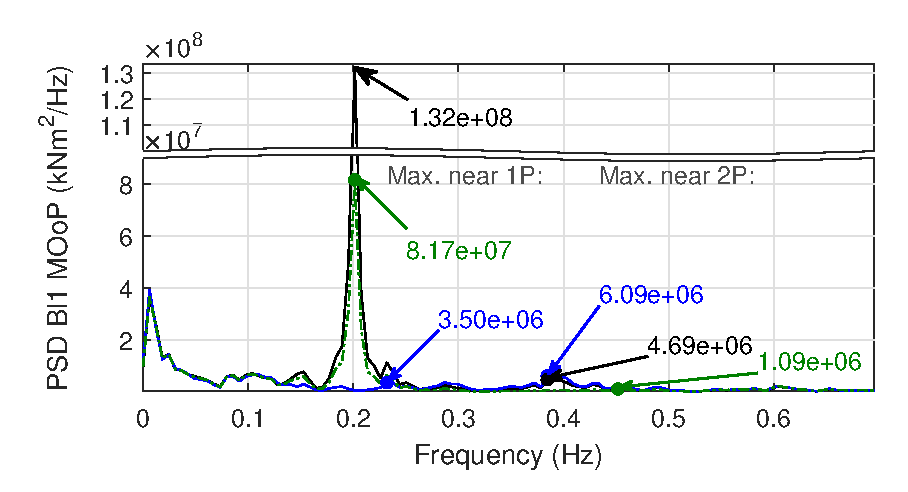
\includegraphics[width=0.65\textwidth]{figures/figIPCThesis/fig02_PSDroot_breaky_AALCinit.eps}}\\
    \subfloat[Baseline (\mBlack), AALC (\mlRed), and AALC optimized (\mlPink)]{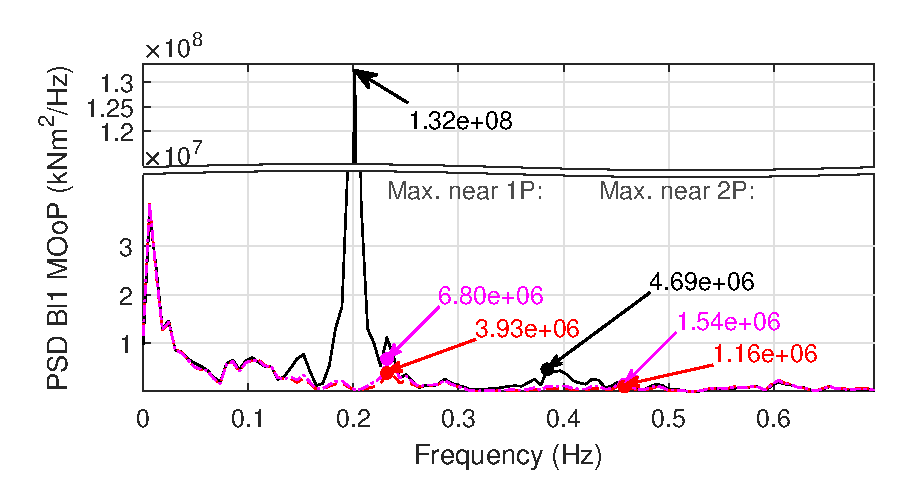
\includegraphics[width=0.65\textwidth]{figures/figIPCThesis/fig02_PSDroot_breaky1c_AALC.eps}}
    \caption[Controller comparison: Power Spectral Density of the blade~1 root out-of-plane moment of baseline PI, IPC, TEFC, AALC, and AALC with optimized parameters.]{Controller comparison: Power Spectral Density of the blade~1 root out-of-plane moment of baseline PI, IPC with $K_{\text{I,IPC}} = 1$, TEFC with $K_{\text{P,TEFC}} = 1$, AALC with $K_{\text{I,IPC}} = 1$ and $K_{\text{P,TEFC}} = 1$, and AALC with optimized parameters \(K_{\text{P,IPC}}\), \(K_{\text{I,IPC}}\), and \(K_{\text{P,TEFC}}\), see Table~\ref{tabone}. Results for turbulent wind (18 m/s mean, turbulence class A, optimization dataset).}
    \label{fig:PSDTEF}
\end{figure}
%
IPC (blue line) and TEFC (green line) reduce the PSD of the 1P and 2P loads, respectively, compared to the baseline (black line): IPC alone reduces the 1P peak by 97.4\%, but increases the 2P peak by 29.8\%, while TEFC alone reduces the 2P peak by 76.8\% and the 1P peak by 38.3\%. These PSDs are obtained with the initially used AALC parameters with the original setting of a purely integral IPC and a purely proportional TEFC feedback, both set to values of one. In a second step, the three parameters \(K_{\text{P,IPC}}\), \(K_{\text{I,IPC}}\), and \(K_{\text{P,TEFC}}\) are optimized at 18\,m/s, subject to the constraint that the tower base DEL does not exceed that of the baseline, resulting in an IPC PI controller with $K_{\text{P,IPC}} = 0.082$ and $K_{\text{I,IPC}} = 0.669$ and a TEFC P controller with $K_{\text{P,TEFC}} = 0.641$. An optimization started from the initial parameters instead of the optimized IPC parameters converges to the same cost.

Figure~\ref{fig:PSDTEF}\,(b) demonstrates that considerable improvement with respect to the baseline controller is possible using the suggested AALC design: The combined IPC-TEFC with the original setting of a purely integral IPC and proportional TEFC feedback reduces the PSD at 1P by 97.0\%, and at 2P by 75.3\%. With the optimized parameters, the reduction with respect to the baseline is 94.9\% at 1P and 67.3\% at 2P, i.e., the residual peaks are larger than with the initial setting. The cost function, the largest of the three blade DELs, is nevertheless decreased from $J = 0.778$ for the initial controller to $J = 0.773$ for the optimized one, as the optimized controller reduces the DELs of the three blades more evenly (by 22.7\% to 23.3\%, compared to 22.2\% to 25.1\% with the initial setting). At the same time, the optimized AALC requires less pitch activity than the optimized IPC without TEF: the standard deviation of the pitch rate is 2.14\textdegree/s compared to 2.98\textdegree/s.
From this study, it seems unlikely that a parameter optimization of the suggested, carefully designed controller can decrease the blade damage equivalent loads considerably further. Further investigations might be made with respect to how much improvement is achievable with a more sophisticated MIMO controller.

%
Table~\ref{tabone} contains six evaluation criteria to quantify the effect of the AALC: blade, tower base, and tower top DEL, mean of generated power $\bar{P}_{g}$, its standard deviation $\delta P$, and actuator power $C_{\text{Act}}$, Equation~\eqref{eq:CAct}, normalized by simulations without AALC for the same wind test cases. These are the criteria provided in Section~\ref{sec:ControllerParameterOptimization}, which are the same objectives shown for IPC without TEFs in Table~\ref{tab:IPC_summary} for wind speed ranges for above rated wind. For that table, the parameters are fixed. Here they vary as follows:
\begin{itemize}
    \item For wind speeds of 10\,m/s and above, the parameters optimized at 18\,m/s ($K_{\text{P,IPC}} = 0.082$, $K_{\text{I,IPC}} = 0.669$, and $K_{\text{P,TEFC}} = 0.641$) are used.
    \item For the datasets with wind speeds of 4\,m/s, 6\,m/s, and 8\,m/s, the AALC parameters are scheduled with the parameters optimized separately. The parameters were set to
    \begin{itemize}
        \item for  4\,m/s to $K_{\text{P,IPC}} = 0.422$,  $K_{\text{I,IPC}} = 0.959$,  $K_{\text{P,TEFC}} =  2.028$,
        \item for  6\,m/s to $K_{\text{P,IPC}} =2.038$,  $K_{\text{I,IPC}} = 1.437$,  $K_{\text{P,TEFC}} = 2.970$, and
        \item for  8\,m/s to $K_{\text{P,IPC}} =-0.043$,  $K_{\text{I,IPC}} = 0.826 $,  $K_{\text{P,TEFC}} = 4.939$.
    \end{itemize}
\end{itemize}
These controllers are applied on FAST and the criteria are calculated from the obtained closed-loop data. Averages over five wind speed ranges are derived: all wind speeds, the wind speeds below and above rated, the wind speeds from 18\,m/s, and the optimization wind speed of 18\,m/s. Unlike in \cite{dittmer2024combined}, where W\"ohler exponents of 8 and 3 were used, the DELs are calculated with the exponents of 10 and 4 used throughout this thesis and evaluated from 60\,s onward, so that the values differ from those published there.
% \caption[Evaluation criteria for IPC: Mean values of the optimization and verification datasets over above rated wind speed ranges]{\label{tab:IPC_summary} Evaluation criteria for IPC: Mean values of the optimization and verification datasets over above rated wind speed ranges, normalized by the baseline PI without IPC; values below 1 indicate a reduction. IPC gains optimized at 18\,m/s with the pitch rate limit 8\textdegree/s for all wind speeds: $K_{\text{P,IPC}} = 1.222$ and $K_{\text{I,IPC}} = 0.370$. Criteria are blade, tower base and tower top DELs, power mean and standard deviation, and pitch actuator power. The first verification set has no wind field for 13\,m/s.}

% Created by makeAALC_SummaryTable on 2026-10-26
\begin{table}[h]
    \centering
    
    \caption[Evaluation criteria for AALC: Mean values of the optimization and verification datasets over different wind speed ranges.]{Evaluation criteria for AALC: Mean values of the optimization and verification datasets over different wind speed ranges, normalized by the baseline PI; values below 1 indicate a reduction. From 10\,m/s on, the AALC gains optimized at 18\,m/s are used: $K_{\text{P,IPC}} = 0.082$, $K_{\text{I,IPC}} = 0.669$ and $K_{\text{P,TEFC}} = 0.641$; below, the gains are scheduled with the gains optimized at 4, 6 and 8\,m/s. Criteria are blade, tower base and tower top DELs, power mean and standard deviation, and pitch actuator power (not given below rated, where the baseline actuator power is close to zero). The first verification set has no wind fields for 11 and 13\,m/s.}
    \begin{tabular}{@{}l*{8}{c}@{}}
        \toprule
        Wind speeds & Dataset & Turb. class & $C_{\text{DEL},b}$ & $C_{\text{DEL},t,\text{Base}}$ & $C_{\text{DEL},t,\text{Top}}$ & $C_{\bar{P}}$ & $C_{\delta P}$ & $C_{\text{Act}}$ \\
        \midrule
        \multirow{3}{*}{All (4--25\,m/s)} & Optim. & A & 0.77 & 0.98 & 0.89 & 0.99 & 1.02 & 4.54 \\
        & Verif. 1 & A & 0.84 & 0.98 & 0.91 & 0.99 & 1.00 & 4.60 \\
        & Verif. 2 & B & 0.80 & 0.99 & 0.89 & 0.99 & 1.00 & 4.73 \\
        \midrule
        \multirow{3}{*}{\begin{tabular}[c]{@{}l@{}}Below rated\\(4--11\,m/s)\end{tabular}}& Optim. & A & 0.80 & 0.94 & 0.89 & 0.98 & 1.00 & -- \\
        & Verif. 1 & A & 0.98 & 0.93 & 0.93 & 0.97 & 0.98 & -- \\
        & Verif. 2 & B & 0.84 & 0.96 & 0.89 & 0.98 & 0.98 & -- \\
        \midrule
        \multirow{3}{*}{\begin{tabular}[c]{@{}l@{}}Above rated\\(12--25\,m/s)\end{tabular}} & Optim. & A & 0.76 & 1.00 & 0.89 & 1.00 & 1.02 & 3.86 \\
        & Verif. 1 & A & 0.77 & 1.00 & 0.90 & 1.00 & 1.01 & 3.85 \\
        & Verif. 2 & B & 0.78 & 1.01 & 0.89 & 1.00 & 1.02 & 4.02 \\
        \midrule
        \multirow{3}{*}{18--25\,m/s} & Optim. & A & 0.74 & 1.00 & 0.90 & 1.00 & 1.00 & 3.99 \\
        & Verif. 1 & A & 0.74 & 1.00 & 0.92 & 1.00 & 1.00 & 3.89 \\
        & Verif. 2 & B & 0.73 & 1.02 & 0.91 & 1.00 & 1.00 & 4.19 \\
        \midrule
        \multirow{3}{*}{18\,m/s} & Optim. & A & 0.79 & 1.00 & 0.86 & 1.00 & 0.99 & 3.64 \\
        & Verif. 1 & A & 0.79 & 1.00 & 0.90 & 1.00 & 1.00 & 3.49 \\
        & Verif. 2 & B & 0.78 & 1.06 & 0.87 & 1.00 & 1.00 & 3.77 \\
        \bottomrule
    \end{tabular}
    \label{tabone}
\end{table}

While load reduction is also achievable below rated wind speed, Table~\ref{tabone} shows that the control parameters that worked well on the optimization set reduced the loads on the first verification set only marginally: the blade DEL is reduced by 20\% for the optimization set and by 16\% for the second verification set, but only by 2\% for the first verification set, i.e., the parameters optimized below rated do not carry over reliably to other wind fields. As the baseline pitch angle is almost constant for below rated wind speeds, the baseline actuator power is close to zero and no meaningful ratio is obtained for the actuator criterion. Nevertheless, some improvements can be seen: the tower base DEL is reduced by 4\% to 7\% and the tower top DEL by 7\% to 11\%. For all datasets, a decrease in power is observed: the mean power is decreased by 2\% to 3\%, as the flap and pitch deflections reduce the aerodynamic efficiency, see Figure~\ref{fig:OLval}. This makes the application of TEFs during periods with below rated wind speeds economically non-viable. No further investigation of finding suitable controller parameters for this range is hence conducted.

The following analysis focuses on the above rated wind speed ranges. The reduction values achieved with IPC without TEFs from Table~\ref{tab:IPC_summary} are also provided here for direct comparison. The blade root out-of-plane moments, quantified with the criterion $C_{\text{DEL},b}$, the sum of the blade DELs, decrease as follows:
\begin{itemize}
    \item For the mean value of all above rated wind speeds, compared to the baseline PI, the blade DEL criterion $C_{\text{DEL},b}$ decreases by 22\% (on the second verification set) to 24\% (on the optimization set). The corresponding reductions achieved by IPC are 21\% to 23\%. 
    \item If only wind speeds from 18\,m/s on are considered, the loads are decreased by 26\% (on the two sets with turbulence class A) to 27\% (on the set with turbulence class~B), with the corresponding reduction range for IPC being 24\% to 25\%.
    \item Finally, if only the runs with a wind speed of 18~m/s are considered, which includes the optimization set that was used to derive the controller parameters, the reduction amounts to 21\% to 22\%, with the largest reduction again observed for the second verification set of turbulence class~B. 
\end{itemize} 
Including all wind speeds, the blade DEL is reduced by 16\% to 23\%. The parameters optimized at a single wind speed carry over to the whole of Region~III and to both verification sets, so that no gain scheduling is required above rated. Compared to the load reduction achieved with IPC, a small further improvement of up to 2 percentage points is observed for the objective $C_{\text{DEL},b}$.
%
Regarding the tower DELs, quantified with the objectives $C_{\text{DEL},t,\text{Base}}$ and $C_{\text{DEL},t,\text{Top}}$, the following influence of the AALC is observed:
\begin{itemize}
    \item The tower base DEL is not changed considerably above rated, with criteria between 1.00 and 1.01; the largest increase of a single wind speed is 6\% at 18\,m/s for turbulence class~B. Above rated and at 18\,m/s, the IPC values in Table~\ref{tab:IPC_summary} happen to be identical to the AALC ones in Table~\ref{tabone} for this objective.
    \item The tower top DEL, in contrast, is reduced by 10\% to 11\% on average above rated, 8\% to 10\% for the wind speed range above 18\,m/s, and by 10\% to 14\% at 18\,m/s. This is noticeably more than by the IPC alone, where the corresponding numbers are 7\% above rated, 5\% to 7\% and 8\% to 10\%. 
\end{itemize}
%
The evaluation of the power criteria confirms that the AALC leads only to negligible changes in both power mean and variance above rated. The additional movement of the blade demanded by the IPC component of the AALC is the only criterion leading to an unavoidable increase, similar to the IPC scheme discussed in the previous sections. However, the objective $C_{\text{Act}}$ is another criterion where AALC outperforms IPC: 
\begin{itemize}
    \item Above rated, the actuator power is increased by a factor of 3.9 to 4.0, and from 18\,m/s on by a factor of 3.9 to 4.2. The corresponding values for IPC are 5.4 to 5.7, and 5.8 to 6.0.
    \item If only the simulations at a wind speed of 18\,m/s are considered, these values are lower as the additional actuator demand increases with higher wind speeds: They are 3.5 to 3.8 for AALC and 5.0 for IPC.
\end{itemize}
In summary, when considering above-rated wind speeds, AALC outperforms IPC: it provides an additional reduction in blade DELs of up to 2 percentage points and in tower top DELs of up to 4 percentage points, and it decreases the actuator criterion $C_{\text{Act}}$ by about 30\%. To assess the overall performance of AALC and IPC with regard to the qLMPC CPC scheme, the following section presents a comparison of all three investigated algorithms on load reduction and power standard deviation at different pitch rate limits.


%The resulting closed loop simulation results are referred to in this chapter as qLMPC (Mdl2), qLMPC (FAST) and qLMPC smooth (FAST). All of them were tested with three different pitch rate limits,  4\textdegree/s, 8\textdegree/s, and 13\textdegree/s.
%\item 

\section{Comparison of Wind Turbine Control Designs}
\label{subsec:ComparisonWindTurbineControlDesigns}

Three different control approaches were discussed in this chapter: In Section~\ref{sec:quasiLPVMPCDesign} a qLMPC algorithm was presented and applied to a qLPV model without any model mismatch as well as to FAST. Tested on the qLPV model, it resulted in considerable reduction of the standard deviation of the tower fore-aft acceleration, rotor speed and power. It was shown that there is a trade-off between these objectives and pitch actuation by testing the qLMPC with three different pitch rate limits, but that the qLMPC outperformed the baseline PI at all three rate limits. However, when tested on FAST, the original design performed considerably worse regarding rotor speed and power. Some of the performance improvement could be recovered by adapting and enhancing the MPC. 

Section~\ref{section:Individal Pitch PI Control} presented the optimization of an IPC PI controller that was run in addition to the baseline PI controller. Its performance was also tested with the three pitch rate limits. In Section~\ref{sec:CombinedIPC-TrailingEdgeFlapControl} the addition of TEFs was shown. Optimization of a proportional gain for these additional control surfaces was discussed and the resulting AALC was shown to slightly outperform the IPC with regard to DEL reduction and considerably with regard to actuator activity. The decision was made to only tune the AALC scheme for the standard pitch rate of 8\textdegree/s, which is widely used in the literature, as the IPC exceeds this rate limit only rarely.

This section presents the combination of the qLMPC designs from Section~\ref{sec:quasiLPVMPCDesign} with the IPC implementation from Section~\ref{section:Individal Pitch PI Control} as another approach to alleviate the blade loads as well as reduce power standard deviation at an acceptable increase in actuator activity.
%\end{itemize}
The results achieved with the qLMPC can be summarized as follows. In a first simulative analysis, the qLMPC was evaluated on the simplified qLPV turbine model that is also
used as its prediction model, for turbulent wind with a mean of 18\,m/s. Without any model
mismatch, this qLMPC (Mdl2) data showed large improvements over the PI baseline across all evaluated pitch rate limits.
As presented in Table~\ref{tab:stddev_unified}, 
\begin{list}
    {-}{\setlength{\topsep}{5pt}\setlength{\partopsep}{5pt}\setlength{\itemsep}{0pt}\setlength{\parsep}{0pt}}
    \item the standard deviation of the tower fore-aft acceleration was reduced
    by factors of 2.58, 3.82, and 4.14 for the pitch rate limits of 4\textdegree/s, 8\textdegree/s, and
    13\textdegree/s, respectively.
    %\item  This corresponds  corresponding to reductions of 61\%, 74\%, and 76\% relative to the PI baseline at 8\textdegree/s). 
    \item Similarly, the power error standard deviation dropped dramatically
    by factors of 6.42, 10.29, and 11.35 (reductions between 84\% and 91\%), 
    \item and the rotor speed
    standard deviation showed matching improvements with reductions up to a factor of 11.40 at the
    13\textdegree/s rate limit. 
\end{list}
These improvements did not hold up when the controller was applied to the FAST model of the NREL 5MW
turbine. The original qLMPC design increased the power tracking error instead of reducing it, mainly due to the single-point hub height wind speed used for scheduling, while the FAST rotor averages the fluctuations of a full wind field, and additionally due to the modes of FAST, which are not contained in the prediction model.
%
The improvements were partly recovered with several modifications, namely rotor speed tracking, a prediction model extended by the tower fore-aft and blade flap dynamics, a controller sample time of 0.04\,s, scheduling with the rotor-effective wind speed, notch filters in the measured speeds at the 3P frequency and the drivetrain mode, as well as, for the smooth design, a controller sample time of 0.12\,s and a ramped pitch reference.
%
The smooth design, enhanced with these extensions, reduces the power variance on FAST again. However, the increase in tower
loads was only partially reduced, and the tower DELs remained higher than those obtained with the baseline PI controller. Note that on the simplified model implemented in Simulink, the
rotor-effective wind filters shown in Table~\ref{tab:stddev_unified} have a similar effect: they
remove a large part of the wind excitation. With this, the pitch activity was reduced below that of the baseline PI, but there was a decrease in improvement of the
qLMPC regarding tower acceleration and power standard deviation reduction. 
%
Therefore, the notch filter and smooth designs are combined with the IPC of Section~\ref{section:Individal Pitch PI Control}, with the gains scaled as described in Section~\ref{sec:qLMPCFAST}. Figure~\ref{fig:CtrlCmpFASTIPC} and Table~\ref{tab:CtrlComparisonFASTNTM18B_PI_flapNotch_flapNotchIPC} show the effect of the IPC on the qLMPC notch filter and smooth designs in the time domain. The turbulent wind field of Section~\ref{quasiLPVMPCResults} and a pitch rate limit of 13\textdegree/s are used. Note that the bar and Pareto plots below are based on the second verification set and a pitch rate limit of 8\textdegree/s.
The following can be observed from Figure~\ref{fig:CtrlCmpFASTIPC} where the baseline PI is depicted as a blue line, the qLMPC design as an orange line, and the combination of qLMPC and IPC as a yellow line. Table~\ref{tab:CtrlComparisonFASTNTM18B_PI_flapNotch_flapNotchIPC} summarizes the findings from the comparison of the five controller setups:
\begin{itemize}
    \item All four qLMPC algorithms show a considerable decrease in the standard deviation of rotor speed and power tracking error: Compared to the baseline PI, the standard deviations of the rotor speed and of the power tracking error are reduced by factors of 3.8 and 3.3 without IPC and of 3.7 and 3.3 with IPC. For the smooth design, the factors are 2.1 and 2.0 without and 2.2 and 2.0 with IPC. Regarding these criteria, adding the IPC has little influence on the already good improvement.
    \item  The tower acceleration and the tower base DEL increase slightly further by 4\%: without IPC, they are increased by 35\% and 27\%, with IPC by 40\% and 31\%. For the smooth design, the increases are smaller, 16\% and 12\% without and 20\% and 15\% with IPC.
    \item  However, the qLMPC-IPC, like the PI IPC, reduces the standard deviation of the blade root out-of-plane moment by 23\% and the blade DEL by 18\%, i.e.\ to 14\% below that of the baseline PI controller. For the smooth design, the reductions are 23\% and 19\%, i.e.\ to 19\% below the baseline. 
    \item The trade-off is that adding the IPC increases the blade 1 pitch rate by 15\%, to 6.2 times that of the baseline PI (5.4 without IPC). For the smooth design, the pitch rate is considerably lower, 2.3 times that of the baseline without and 3.9 times with IPC.  
\end{itemize}
Both combined qLMPC-IPC designs are thus able to reduce the power standard deviation and the blade DEL. The latter was not achieved with the qLMPC with collective pitch control. However, these improvements come at the price of a further, albeit small, increase in tower DEL and a considerable increase in pitch rate, both of which are smaller for the smooth design.
%
\begin{figure} [htbp]
    \subfloat[Notch filter design]{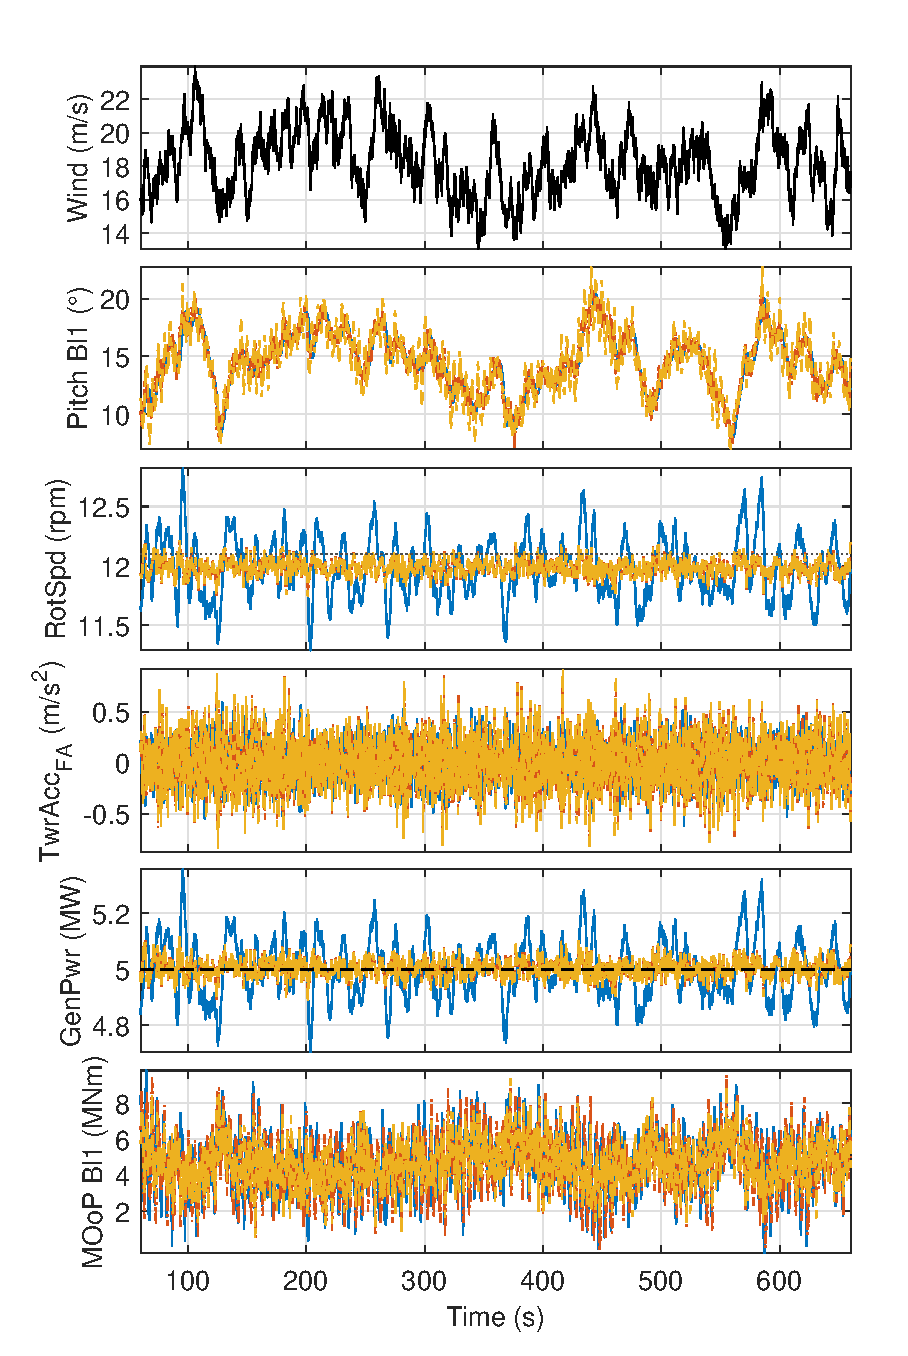
\includegraphics[width=0.495\textwidth,trim={0.cm 0cm 0cm 0.5cm}, clip]{figures/figDirFASTthesis/cmpCtrlFASTthesis_NTM18B_PI_flapNotch_flapNotchIPC.eps}}\hfill
    \subfloat[Smooth design]{\includegraphics[width=0.495\textwidth,,trim={0.cm 0cm 0cm 0.5cm}, clip]{figures/figDirFASTthesis/cmpCtrlFASTthesis_NTM18B_PI_flapNotchSmooth12_flapNotchSmooth12IPC.eps}}\hfill
    \caption[Controller comparison on FAST: baseline PI vs. qLMPC designs without and with IPC for turbulent wind (18\,m/s mean, turbulence class B).]
    {Controller comparison on FAST: baseline PI (\mlBlue) vs. qLMPC designs without (\mlOrange) and with IPC (\mlYellow) for turbulent wind (18\,m/s mean, turbulence class B), pitch rate limit 13\textdegree/s. Displayed signals: freestream wind speed, generator torque, blade 1 pitch angle, rotor speed, tower fore-aft acceleration, generator power with its reference (\mlBlackDashed), and blade 1 root out-of-plane moment.}
    \label{fig:CtrlCmpFASTIPC}
\end{figure}
%
\begin{table}[htbp]
    \centering
    \small
    \setlength{\tabcolsep}{4pt}
    \caption[Controller comparison on FAST, 18\,m/s turbulent (class B): notch filter design and smooth design, each without and with IPC.]{Controller comparison on FAST v8.16, 18\,m/s turbulent (class B), pitch rate limit 13\textdegree/s, notch filter design and smooth design, each without and with IPC. Top: standard deviations of the tower fore-aft acceleration, the power tracking error, the rotor speed, the blade 1 pitch rate (differenced over 0.04\,s), and the blade root out-of-plane (OoP) moment (mean of the blades). Bottom: damage equivalent loads of the tower base (W\"ohler exponent 4) and the blade root (exponent 10, maximum of the blades). Values in parentheses: ratio of the baseline PI value to the controller value; values above 1 indicate an improvement. Best values are marked in bold.}
    \label{tab:CtrlComparisonFASTNTM18B_PI_flapNotch_flapNotchIPC}
    \begin{tabular}{l rrrrr}
        \toprule
        &  & \multicolumn{2}{c}{Notch filter design} & \multicolumn{2}{c}{Smooth design} \\
        \cmidrule(lr){3-4} \cmidrule(lr){5-6}
        Signal & Baseline PI & w/o IPC & w/ IPC & w/o IPC & w/ IPC \\
        \midrule
        Tower acc.\ (m/s$^2$) & \textbf{0.1712} & 0.2310 (0.74) & 0.2393 (0.72) & 0.1990 (0.86) & 0.2046 (0.84) \\
        Power error (kW) & 59.60 & \textbf{17.90 (3.33)} & 18.08 (3.30) & 29.18 (2.04) & 29.08 (2.05) \\
        Rotor speed (rpm) & 0.2460 & \textbf{0.0653 (3.77)} & 0.0660 (3.73) & 0.1145 (2.15) & 0.1141 (2.16) \\
        Blade 1 pitch rate (\textdegree/s) & \textbf{0.50} & 2.71 (0.18) & 3.11 (0.16) & 1.16 (0.43) & 1.93 (0.26) \\
        Blade root OoP moment (kNm) & 1574 & 1559 (1.01) & 1207 (1.30) & 1548 (1.02) & \textbf{1188 (1.32)} \\
        \midrule
        Tower base DEL (kNm) & \textbf{15394} & 19493 (0.79) & 20232 (0.76) & 17172 (0.90) & 17728 (0.87) \\
        Blade root DEL (kNm) & 6002 & 6249 (0.96) & 5145 (1.17) & 6019 (1.00) & \textbf{4871 (1.23)} \\
        \bottomrule
    \end{tabular}
\end{table}
%
All seven designs are compared for the same wind, the turbulent 18\,m/s wind of the
second verification set (IEC turbulence class~B), with the pitch rate limits 4\textdegree/s,
8\textdegree/s, and 13\textdegree/s. The qLMPC is evaluated on the simplified model Mdl2 as the
ideal case without model mismatch, and on FAST with the filter designs, both on their own
and combined with the individual pitch controller of Section~\ref{section:Individal Pitch PI Control}.
IPC and AALC are evaluated on OpenFAST with the optimized gains for each rate limit and the
AALC gains of Section~\ref{subsec:ResultsTEF} at 8\textdegree/s. All criteria are normalized by the
PI baseline on the same plant and with the same pitch rate limit, so values below unity
indicate an improvement. The blade DEL and the DELs of the tower base and the tower top fore-aft moments are computed by
rainflow counting with W\"ohler exponents of 10 for the blades, summed over the three blades, and
4 for the steel tower; all criteria are evaluated from 60\,s onwards to exclude the start-up. Mdl2 contains neither blade loads nor a pitch moment.


For the qLMPC on Mdl2, the standard deviation of the
tower top fore-aft acceleration replaces the tower base DEL, no blade and tower top DELs are given, and $C_\text{Act}$ is calculated with a pitch moment estimated from the pitch angle, its derivatives, and the wind speed, fitted by least squares to the pitch moment of blade~1 in the FAST runs of the PI and the notch filter design at 8\textdegree/s. The fit explains only a quarter of the variance of the pitch moment ($R^2 = 0.25$); most of the remaining variance lies around the rotational frequency 1P, which depends on the blade azimuth and cannot be represented by the collective signals of Mdl2. The actuator power is nevertheless reproduced within 0.3\% for the qLMPC designs on FAST, as the pitch moment is dominated by its nearly constant mean value of about $-86$\,kNm, which is the same for all controllers. $C_\text{Act}$ is therefore essentially the ratio of the mean absolute pitch rates: on FAST, the two differ by less than 2\%, and for the qLMPC on Mdl2 by less than 0.5\%.

Figure~\ref{fig:CtrlCompBarPareto}(a) shows the evaluation criteria of all controllers at the standard
pitch rate limit of 8\textdegree/s, grouped by controller. It is important to note that no controller changes the mean power
$C_{\bar{P}}$ depicted in gray as the fourth bar; all values are within 0.5\% of the baseline and hence, with only the first two digits displayed, the bar appears to be exactly at the value of one for all seven algorithms. Figure~\ref{fig:CtrlCompBarPareto}(b) disregards the mean power criterion and visualizes the three DEL criteria and the power standard deviation as functions of the actuator power for all three pitch rate limits. Each line connects the
results of one controller for the rate limits of 4\textdegree/s, 8\textdegree/s, and 13\textdegree/s,
indicated by white, gray, and black marker fill. The AALC was optimized for 8\textdegree/s only and
is therefore represented by a single point per criterion. Results closer to the lower left corner
are better, as they combine lower loads or power variance with less actuator activity. Each panel
highlights one group of controllers and shows the others pale for reference.

\begin{figure}[htbp]
    \centering
    \subfloat[Bar plot at a pitch rate limit 8\textdegree/s\label{fig:EvalCrit1}]{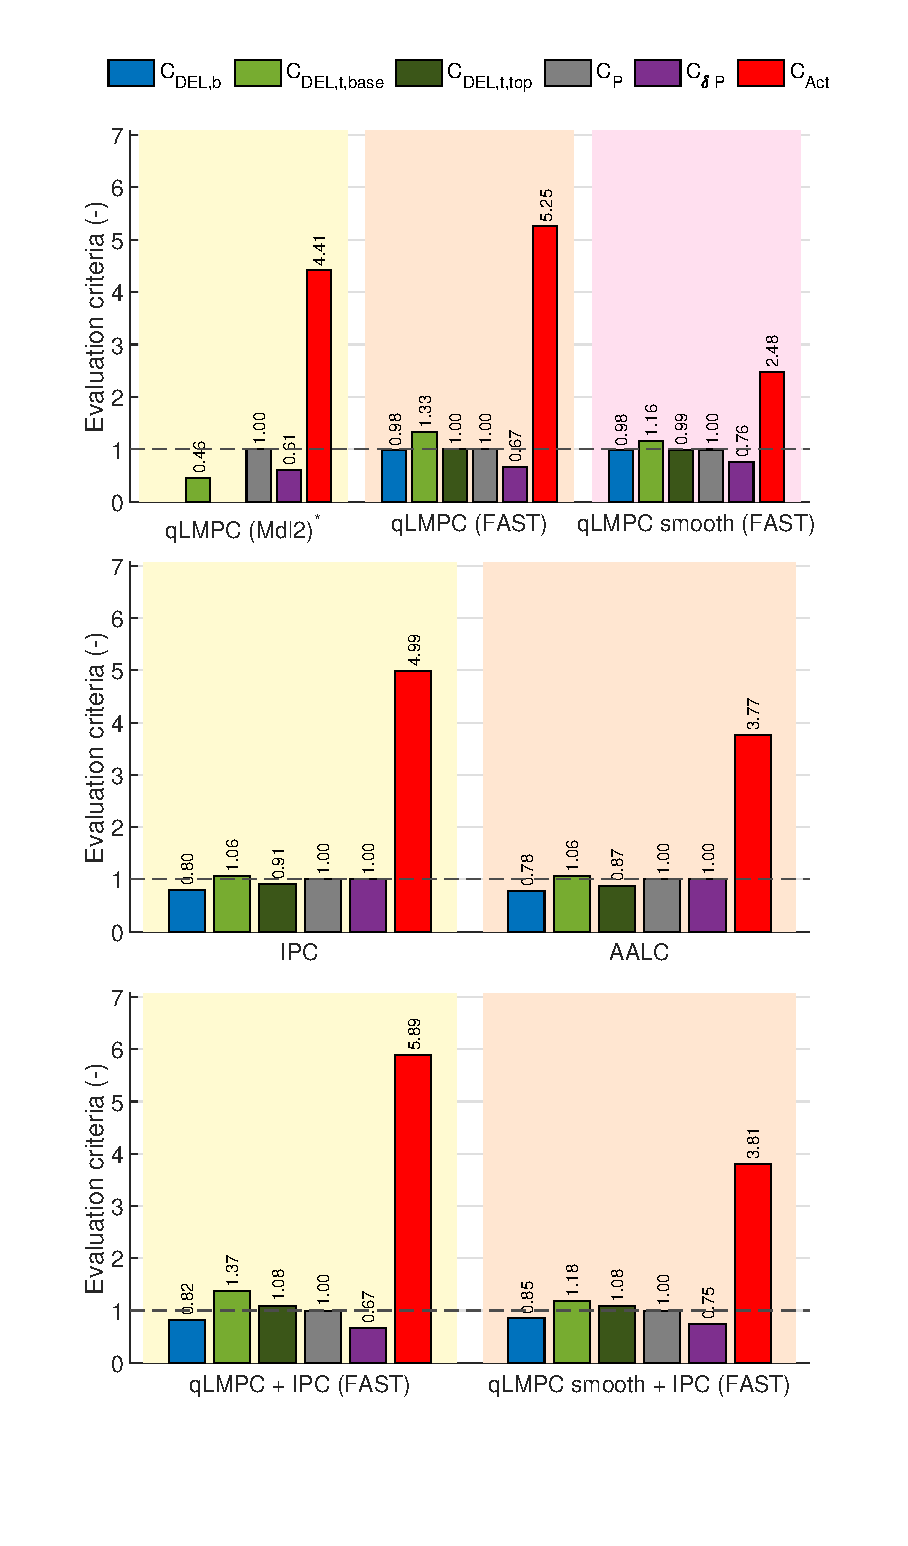
\includegraphics[width=0.499\textwidth]{figures/figures_WESC25/afig01_IPCMPCbar.eps}}\hfill
    \subfloat[Pareto plot\label{fig:CtrlCompAll}]{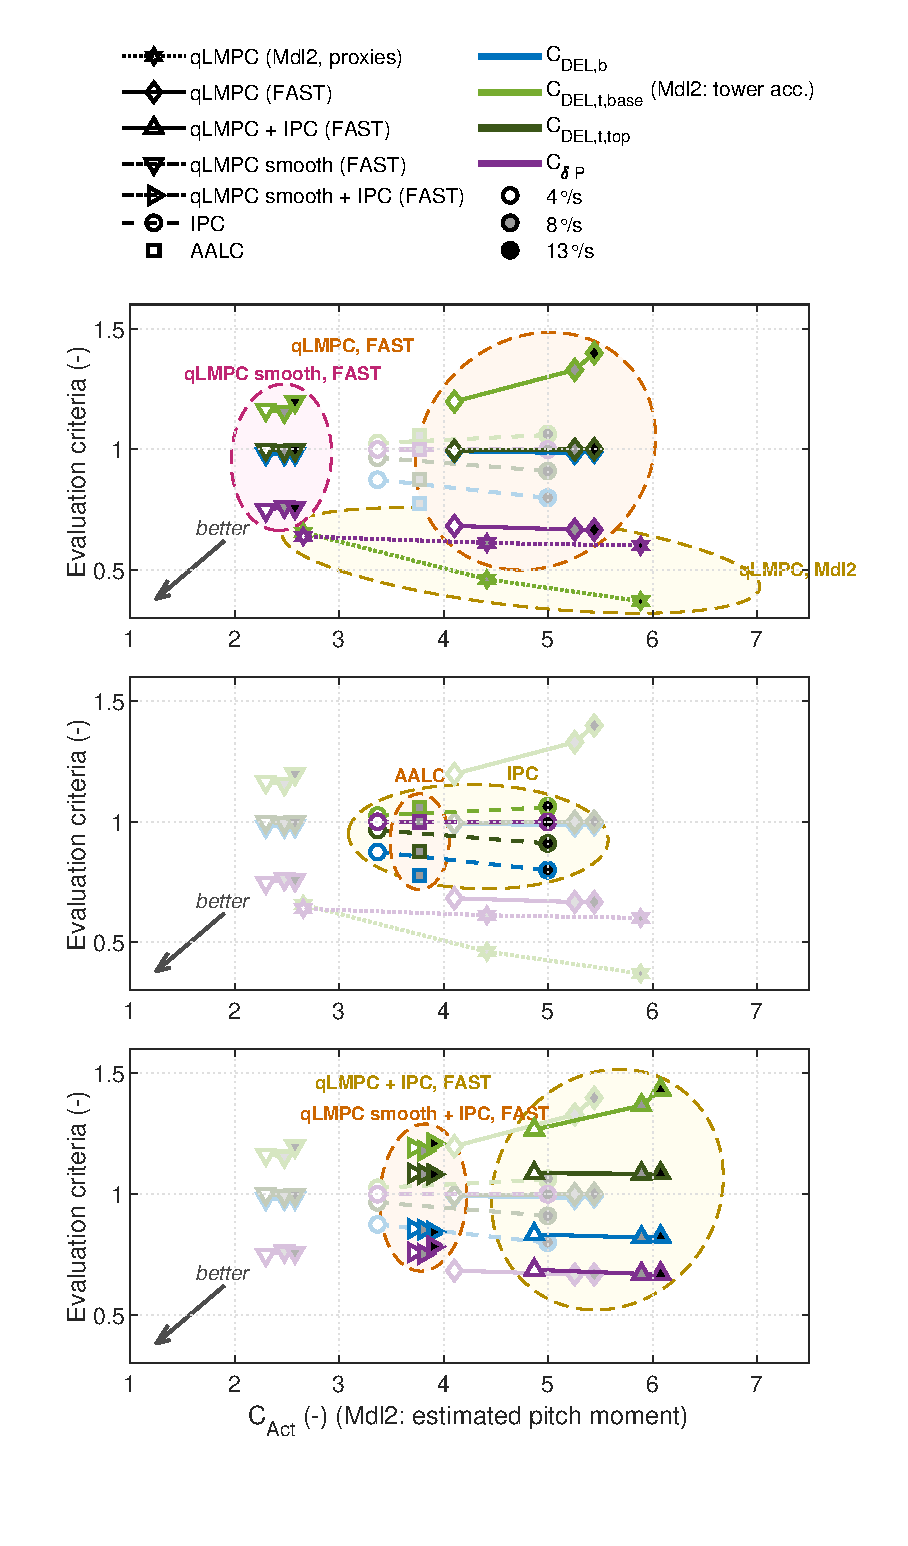
\includegraphics[width=0.499\textwidth]{figures/figures_WESC25/afig01_IPCMPCpareto.eps}}
    \caption[Evaluation criteria of qLMPC, IPC, and AALC for turbulent wind]{Evaluation criteria of the controllers for turbulent wind (18\,m/s mean, IEC turbulence class~B, second verification set), normalized by the PI baseline with the same pitch rate limit. Panels: qLMPC (top), IPC and AALC (middle), qLMPC combined with IPC (bottom). (a)~Bar plots: blade DEL $C_{\mathrm{DEL},b}$, tower base and top DELs $C_{\mathrm{DEL},t,\mathrm{Base}}$ and $C_{\mathrm{DEL},t,\mathrm{Top}}$, mean power $C_{\bar{P}}$, power standard deviation $C_{\delta P}$, and actuator power $C_\text{Act}$. (b)~Pareto plot: $C_{\mathrm{DEL},b}$ (blue), $C_{\mathrm{DEL},t,\mathrm{Base}}$ (green), $C_{\mathrm{DEL},t,\mathrm{Top}}$ (dark green), and $C_{\delta P}$ (purple) over $C_\text{Act}$ for the pitch rate limits 4\textdegree/s (white markers), 8\textdegree/s (gray), and 13\textdegree/s (black); the controllers of the other panels are shown pale. The dashed ovals enclose all points of one controller; their color matches the background of the same controller in the same panel of the bar plot. The qLMPC on Mdl2 (no model mismatch): tower top fore-aft acceleration instead of the tower base DEL, no blade and tower top DELs, $C_\text{Act}$ with the pitch moment estimated from a model fitted to FAST. The arrow points towards better results.}
    \label{fig:CtrlCompBarPareto}
\end{figure}
The two top panels show the qLMPC schemes. On Mdl2, i.e.\ without model mismatch (yellow background), the power standard deviation is reduced by 39\% and the standard deviation of the tower fore-aft acceleration by 54\%. This is the setup used in \cite{dittmer2021velocity} to investigate the potential of the velocity-based qLMPC. The Verif.~2 wind field differs from the test case of Section~\ref{quasiLPVMPCResults} and falls below rated wind speed several times, so the improvements are smaller than the 74\% and 90\% reported there at 8\textdegree/s. The actuator power increases by a factor of 4.4, as the qLMPC compensates the wind fluctuations with fast pitch action, which might well be worth the additional actuator usage. These improvements, however, could not be replicated on FAST (orange background): the qLMPC with notch filters still reduces the power standard deviation by 33\%, but increases the tower DEL by 33\% and requires the highest actuator power of all controllers without IPC, 5.3 times that of the PI baseline. The smooth design (pink), which uses a longer controller sample time and a ramped pitch reference to make the qLMPC less aggressive, trades part of the power smoothing, a reduction by 24\%, for considerably less pitch activity: its actuator power of 2.5 is the lowest of all controllers, and the tower DEL increase is halved to 16\%.

The middle panels visualize the IPC and the AALC, which act on the blade loads. The IPC, highlighted with a wider, yellowish oval as it was optimized for each rate limit, reduces the blade DEL from 0.87 at 4\textdegree/s to 0.80 at 8\textdegree/s; 13\textdegree/s brings no further benefit, as the gains optimized for 13\textdegree/s and 8\textdegree/s are almost identical. The tower DEL increases slightly with the rate limit, from 1.03 to 1.06, and the power standard deviation remains at unity. The AALC lies below the IPC curve, i.e., it achieves the larger blade load reduction at a lower pitch actuator power, 3.8 compared with 5.0, as the trailing edge flaps take over part of the load reduction. This is its main advantage, as the further reduction is only 2\% for the blade DEL and 4\% for the tower top DEL.

The bottom panels depict the combination of qLMPC and IPC. Compared with the pale qLMPC curves, adding IPC mainly shifts the blade DEL downwards and the actuator power to the right, while the tower base DEL and the power standard deviation hardly change and the tower top DEL increases by about 8\%. The smooth design combined with IPC lies at about the actuator power of the AALC, 3.8, and below that of the IPC, 5.0. Its blade DEL of 0.85 comes close to the 0.80 of the IPC alone, and it additionally reduces the power standard deviation by about 25\%, which neither IPC nor AALC achieve. As the IPC gains were only scaled by hand on the notch filter design and not retuned for the smooth design (Section~\ref{sec:qLMPCFAST}), part of the remaining blade DEL difference may be due to the tuning. Its tower DEL, however, is about 11\% higher than with IPC.

These summary plots show that IPC and AALC are the two investigated approaches suitable for blade load reduction, with AALC achieving the best blade DEL at a moderate actuator power by offloading part of the pitch action onto the trailing edge flaps. The qLMPC is the only approach that reduces the power variance, and it keeps this property in the presence of model mismatch, with a reduction of about a third on FAST compared with about 40\% on Mdl2. Its tower load reduction without model mismatch, however, is lost on FAST, where all qLMPC designs increase the tower DEL. The smooth qLMPC combined with IPC is the most balanced qLMPC variant, reducing both the blade DEL and the power standard deviation at an actuator power comparable to IPC and AALC.
%
These results show that the qLMPC depends on an accurate representation of the wind acting on the rotor and of the turbine dynamics: despite careful tuning and additional filters, the tower DEL reduction could not be transferred to FAST. A relatively low-hanging fruit would be to stitch a qLPV model from linearized FAST models to investigate whether the additional modes reduce the model mismatch and at least partly recover the tower DEL reduction. Furthermore, all qLMPC designs use the hub height wind speed of the wind field, filtered on FAST, i.e., the wind is assumed to be known exactly. Replacing it with an estimate is a necessary next step, while a wind preview, e.g., from a lidar, combined with a better fitting model might further reduce the loads.
%
IPC, in contrast, reduces the loads without wind measurements or additional actuation hardware. The IPC and AALC controllers were tuned to reduce the blade loads and achieved considerable reductions for both the optimization and the verification datasets. The tower DEL, so far only a constraint and evaluation criterion, could additionally be included as an optimization objective. As the AALC reduces the blade DEL only 2\% more than IPC alone, its main benefit is the lower pitch actuator power, although the power of the flap actuators is not included in this comparison, and it is questionable whether the additional TEF hardware is justified for current turbine sizes. With increasing turbine size, however, reducing the loads without further increasing the actuator power might become more attractive.

The presented qLMPC exploits that individual wind turbine dynamics are well understood and can be described in closed form as low-dimensional nonlinear ODEs. The following chapter discusses data-driven MPC for wind farms, where wake dynamics are time- and location-dependent and cannot be described by closed-form ODEs, yet must be accounted for in any MPC formulation.